\documentclass[a4paper]{book}
\usepackage{makeidx}
\usepackage{graphicx}
\usepackage{multicol}
\usepackage{float}
\usepackage{listings}
\usepackage{color}
\usepackage{ifthen}
\usepackage[table]{xcolor}
\usepackage{textcomp}
\usepackage{alltt}
\usepackage{ifpdf}
\ifpdf
\usepackage[pdftex,
            pagebackref=true,
            colorlinks=true,
            linkcolor=blue,
            unicode
           ]{hyperref}
\else
\usepackage[ps2pdf,
            pagebackref=true,
            colorlinks=true,
            linkcolor=blue,
            unicode
           ]{hyperref}
\usepackage{pspicture}
\fi
\usepackage[utf8]{inputenc}
\usepackage{mathptmx}
\usepackage[scaled=.90]{helvet}
\usepackage{courier}
\usepackage{doxygen}
\lstset{language=C++,inputencoding=utf8,basicstyle=\footnotesize,breaklines=true,breakatwhitespace=true,tabsize=8,numbers=left }
\makeindex
\setcounter{tocdepth}{3}
\renewcommand{\footrulewidth}{0.4pt}
\begin{document}
\hypersetup{pageanchor=false}
\begin{titlepage}
\vspace*{7cm}
\begin{center}
{\Large YDKR }\\
\vspace*{1cm}
{\large Generated by Doxygen 1.7.3}\\
\vspace*{0.5cm}
{\small Sat Jun 25 2011 02:21:30}\\
\end{center}
\end{titlepage}
\clearemptydoublepage
\pagenumbering{roman}
\tableofcontents
\clearemptydoublepage
\pagenumbering{arabic}
\hypersetup{pageanchor=true}
\chapter{Data Structure Index}
\section{Data Structures}
Here are the data structures with brief descriptions:\begin{DoxyCompactList}
\item\contentsline{section}{\hyperlink{structcatalog__change}{catalog\_\-change} }{\pageref{structcatalog__change}}{}
\item\contentsline{section}{\hyperlink{structcatalog__request}{catalog\_\-request} }{\pageref{structcatalog__request}}{}
\item\contentsline{section}{\hyperlink{structcatalog__response}{catalog\_\-response} }{\pageref{structcatalog__response}}{}
\item\contentsline{section}{\hyperlink{structclient__info}{client\_\-info} }{\pageref{structclient__info}}{}
\item\contentsline{section}{\hyperlink{structerror__warning}{error\_\-warning} }{\pageref{structerror__warning}}{}
\item\contentsline{section}{\hyperlink{structerror_m_s_g}{errorMSG} }{\pageref{structerror_m_s_g}}{}
\item\contentsline{section}{\hyperlink{structgame__over}{game\_\-over} }{\pageref{structgame__over}}{}
\item\contentsline{section}{\hyperlink{structglobal__client__info}{global\_\-client\_\-info} }{\pageref{structglobal__client__info}}{}
\item\contentsline{section}{\hyperlink{structlogin__request}{login\_\-request} }{\pageref{structlogin__request}}{}
\item\contentsline{section}{\hyperlink{structlogin__response___o_k}{login\_\-response\_\-OK} }{\pageref{structlogin__response___o_k}}{}
\item\contentsline{section}{\hyperlink{structmsg__header}{msg\_\-header} }{\pageref{structmsg__header}}{}
\item\contentsline{section}{\hyperlink{structplayer__list}{player\_\-list} }{\pageref{structplayer__list}}{}
\item\contentsline{section}{\hyperlink{struct_question}{Question} (Interne Darstellung einer Frage )}{\pageref{struct_question}}{}
\item\contentsline{section}{\hyperlink{structquestion}{question} }{\pageref{structquestion}}{}
\item\contentsline{section}{\hyperlink{structquestion__answered}{question\_\-answered} }{\pageref{structquestion__answered}}{}
\item\contentsline{section}{\hyperlink{structquestion__request}{question\_\-request} }{\pageref{structquestion__request}}{}
\item\contentsline{section}{\hyperlink{structquestion__result}{question\_\-result} }{\pageref{structquestion__result}}{}
\item\contentsline{section}{\hyperlink{struct_question_message}{QuestionMessage} (Darstellung einer Frage während des Transports zum Client )}{\pageref{struct_question_message}}{}
\item\contentsline{section}{\hyperlink{structquestion_result}{questionResult} }{\pageref{structquestion_result}}{}
\item\contentsline{section}{\hyperlink{structstart__game}{start\_\-game} }{\pageref{structstart__game}}{}
\end{DoxyCompactList}

\chapter{File Index}
\section{File List}
Here is a list of all files with brief descriptions:\begin{DoxyCompactList}
\item\contentsline{section}{/home/kathrin/Documents/fh/sysprog/YDKR/source/client/src/\hyperlink{client_8c}{client.c} }{\pageref{client_8c}}{}
\item\contentsline{section}{/home/kathrin/Documents/fh/sysprog/YDKR/source/client/src/\hyperlink{client_2src_2client_8h}{client.h} }{\pageref{client_2src_2client_8h}}{}
\item\contentsline{section}{/home/kathrin/Documents/fh/sysprog/YDKR/source/client/src/\hyperlink{fragewechsel_8c}{fragewechsel.c} }{\pageref{fragewechsel_8c}}{}
\item\contentsline{section}{/home/kathrin/Documents/fh/sysprog/YDKR/source/client/src/\hyperlink{fragewechsel_8h}{fragewechsel.h} }{\pageref{fragewechsel_8h}}{}
\item\contentsline{section}{/home/kathrin/Documents/fh/sysprog/YDKR/source/client/src/\hyperlink{gui_8h}{gui.h} }{\pageref{gui_8h}}{}
\item\contentsline{section}{/home/kathrin/Documents/fh/sysprog/YDKR/source/client/src/\hyperlink{gui__interface_8h}{gui\_\-interface.h} }{\pageref{gui__interface_8h}}{}
\item\contentsline{section}{/home/kathrin/Documents/fh/sysprog/YDKR/source/client/src/\hyperlink{listener_8c}{listener.c} }{\pageref{listener_8c}}{}
\item\contentsline{section}{/home/kathrin/Documents/fh/sysprog/YDKR/source/client/src/\hyperlink{listener_8h}{listener.h} }{\pageref{listener_8h}}{}
\item\contentsline{section}{/home/kathrin/Documents/fh/sysprog/YDKR/source/common/src/\hyperlink{common_2src_2client_8h}{client.h} }{\pageref{common_2src_2client_8h}}{}
\item\contentsline{section}{/home/kathrin/Documents/fh/sysprog/YDKR/source/common/src/\hyperlink{keymanager_8c}{keymanager.c} }{\pageref{keymanager_8c}}{}
\item\contentsline{section}{/home/kathrin/Documents/fh/sysprog/YDKR/source/common/src/\hyperlink{keymanager_8h}{keymanager.h} }{\pageref{keymanager_8h}}{}
\item\contentsline{section}{/home/kathrin/Documents/fh/sysprog/YDKR/source/common/src/\hyperlink{messages_8h}{messages.h} }{\pageref{messages_8h}}{}
\item\contentsline{section}{/home/kathrin/Documents/fh/sysprog/YDKR/source/common/src/\hyperlink{question_8h}{question.h} }{\pageref{question_8h}}{}
\item\contentsline{section}{/home/kathrin/Documents/fh/sysprog/YDKR/source/common/src/\hyperlink{sem_8c}{sem.c} }{\pageref{sem_8c}}{}
\item\contentsline{section}{/home/kathrin/Documents/fh/sysprog/YDKR/source/common/src/\hyperlink{sem_8h}{sem.h} }{\pageref{sem_8h}}{}
\end{DoxyCompactList}

\chapter{Data Structure Documentation}
\hypertarget{structcatalog__change}{
\section{catalog\_\-change Struct Reference}
\label{structcatalog__change}\index{catalog\_\-change@{catalog\_\-change}}
}


{\ttfamily \#include $<$messages.h$>$}

\subsection*{Data Fields}
\begin{DoxyCompactItemize}
\item 
const uint8\_\-t \hyperlink{structcatalog__change_aca7dafb0092715a03dd40f45fc607f2a}{type}
\item 
uint16\_\-t \hyperlink{structcatalog__change_a1892eba2086d12ac2b09005aeb09ea3b}{length}
\item 
char $\ast$ \hyperlink{structcatalog__change_aeac90097f29f7529968697163cea5c18}{filename}
\end{DoxyCompactItemize}


\subsection{Field Documentation}
\hypertarget{structcatalog__change_aeac90097f29f7529968697163cea5c18}{
\index{catalog\_\-change@{catalog\_\-change}!filename@{filename}}
\index{filename@{filename}!catalog_change@{catalog\_\-change}}
\subsubsection[{filename}]{\setlength{\rightskip}{0pt plus 5cm}char$\ast$ {\bf filename}}}
\label{structcatalog__change_aeac90097f29f7529968697163cea5c18}
\hypertarget{structcatalog__change_a1892eba2086d12ac2b09005aeb09ea3b}{
\index{catalog\_\-change@{catalog\_\-change}!length@{length}}
\index{length@{length}!catalog_change@{catalog\_\-change}}
\subsubsection[{length}]{\setlength{\rightskip}{0pt plus 5cm}uint16\_\-t {\bf length}}}
\label{structcatalog__change_a1892eba2086d12ac2b09005aeb09ea3b}
\hypertarget{structcatalog__change_aca7dafb0092715a03dd40f45fc607f2a}{
\index{catalog\_\-change@{catalog\_\-change}!type@{type}}
\index{type@{type}!catalog_change@{catalog\_\-change}}
\subsubsection[{type}]{\setlength{\rightskip}{0pt plus 5cm}const uint8\_\-t {\bf type}}}
\label{structcatalog__change_aca7dafb0092715a03dd40f45fc607f2a}


The documentation for this struct was generated from the following file:\begin{DoxyCompactItemize}
\item 
/home/kathrin/Documents/fh/sysprog/YDKR/source/common/src/\hyperlink{messages_8h}{messages.h}\end{DoxyCompactItemize}

\hypertarget{structcatalog__request}{
\section{catalog\_\-request Struct Reference}
\label{structcatalog__request}\index{catalog\_\-request@{catalog\_\-request}}
}


{\ttfamily \#include $<$messages.h$>$}

\subsection*{Data Fields}
\begin{DoxyCompactItemize}
\item 
const uint8\_\-t \hyperlink{structcatalog__request_aca7dafb0092715a03dd40f45fc607f2a}{type}
\item 
uint16\_\-t \hyperlink{structcatalog__request_a1892eba2086d12ac2b09005aeb09ea3b}{length}
\end{DoxyCompactItemize}


\subsection{Field Documentation}
\hypertarget{structcatalog__request_a1892eba2086d12ac2b09005aeb09ea3b}{
\index{catalog\_\-request@{catalog\_\-request}!length@{length}}
\index{length@{length}!catalog_request@{catalog\_\-request}}
\subsubsection[{length}]{\setlength{\rightskip}{0pt plus 5cm}uint16\_\-t {\bf length}}}
\label{structcatalog__request_a1892eba2086d12ac2b09005aeb09ea3b}
\hypertarget{structcatalog__request_aca7dafb0092715a03dd40f45fc607f2a}{
\index{catalog\_\-request@{catalog\_\-request}!type@{type}}
\index{type@{type}!catalog_request@{catalog\_\-request}}
\subsubsection[{type}]{\setlength{\rightskip}{0pt plus 5cm}const uint8\_\-t {\bf type}}}
\label{structcatalog__request_aca7dafb0092715a03dd40f45fc607f2a}


The documentation for this struct was generated from the following file:\begin{DoxyCompactItemize}
\item 
/home/kathrin/Documents/fh/sysprog/YDKR/source/common/src/\hyperlink{messages_8h}{messages.h}\end{DoxyCompactItemize}

\hypertarget{structcatalog__response}{
\section{catalog\_\-response Struct Reference}
\label{structcatalog__response}\index{catalog\_\-response@{catalog\_\-response}}
}


{\ttfamily \#include $<$messages.h$>$}

\subsection*{Data Fields}
\begin{DoxyCompactItemize}
\item 
const uint8\_\-t \hyperlink{structcatalog__response_aca7dafb0092715a03dd40f45fc607f2a}{type}
\item 
const uint16\_\-t \hyperlink{structcatalog__response_a7767ba464d90fc91ad318d4e182b94d7}{length}
\item 
char $\ast$ \hyperlink{structcatalog__response_aeac90097f29f7529968697163cea5c18}{filename}
\end{DoxyCompactItemize}


\subsection{Field Documentation}
\hypertarget{structcatalog__response_aeac90097f29f7529968697163cea5c18}{
\index{catalog\_\-response@{catalog\_\-response}!filename@{filename}}
\index{filename@{filename}!catalog_response@{catalog\_\-response}}
\subsubsection[{filename}]{\setlength{\rightskip}{0pt plus 5cm}char$\ast$ {\bf filename}}}
\label{structcatalog__response_aeac90097f29f7529968697163cea5c18}
\hypertarget{structcatalog__response_a7767ba464d90fc91ad318d4e182b94d7}{
\index{catalog\_\-response@{catalog\_\-response}!length@{length}}
\index{length@{length}!catalog_response@{catalog\_\-response}}
\subsubsection[{length}]{\setlength{\rightskip}{0pt plus 5cm}const uint16\_\-t {\bf length}}}
\label{structcatalog__response_a7767ba464d90fc91ad318d4e182b94d7}
\hypertarget{structcatalog__response_aca7dafb0092715a03dd40f45fc607f2a}{
\index{catalog\_\-response@{catalog\_\-response}!type@{type}}
\index{type@{type}!catalog_response@{catalog\_\-response}}
\subsubsection[{type}]{\setlength{\rightskip}{0pt plus 5cm}const uint8\_\-t {\bf type}}}
\label{structcatalog__response_aca7dafb0092715a03dd40f45fc607f2a}


The documentation for this struct was generated from the following file:\begin{DoxyCompactItemize}
\item 
/home/kathrin/Documents/fh/sysprog/YDKR/source/common/src/\hyperlink{messages_8h}{messages.h}\end{DoxyCompactItemize}

\hypertarget{structclient__info}{
\section{client\_\-info Struct Reference}
\label{structclient__info}\index{client\_\-info@{client\_\-info}}
}


{\ttfamily \#include $<$client.h$>$}

\subsection*{Data Fields}
\begin{DoxyCompactItemize}
\item 
int \hyperlink{structclient__info_a5903d0b282fc5eae503de618f896b5e1}{sock}
\item 
pthread\_\-t \hyperlink{structclient__info_a01f75a9ad916f63a94e06a27635ba278}{thread}
\item 
char $\ast$ \hyperlink{structclient__info_a5ac083a645d964373f022d03df4849c8}{name}
\item 
uint8\_\-t \hyperlink{structclient__info_af230372c601d9c597265265e9f83f017}{client\_\-id}
\end{DoxyCompactItemize}


\subsection{Detailed Description}
struct das die spielerinfo beinhaltet 

\subsection{Field Documentation}
\hypertarget{structclient__info_af230372c601d9c597265265e9f83f017}{
\index{client\_\-info@{client\_\-info}!client\_\-id@{client\_\-id}}
\index{client\_\-id@{client\_\-id}!client_info@{client\_\-info}}
\subsubsection[{client\_\-id}]{\setlength{\rightskip}{0pt plus 5cm}uint8\_\-t {\bf client\_\-id}}}
\label{structclient__info_af230372c601d9c597265265e9f83f017}
\hypertarget{structclient__info_a5ac083a645d964373f022d03df4849c8}{
\index{client\_\-info@{client\_\-info}!name@{name}}
\index{name@{name}!client_info@{client\_\-info}}
\subsubsection[{name}]{\setlength{\rightskip}{0pt plus 5cm}char$\ast$ {\bf name}}}
\label{structclient__info_a5ac083a645d964373f022d03df4849c8}
\hypertarget{structclient__info_a5903d0b282fc5eae503de618f896b5e1}{
\index{client\_\-info@{client\_\-info}!sock@{sock}}
\index{sock@{sock}!client_info@{client\_\-info}}
\subsubsection[{sock}]{\setlength{\rightskip}{0pt plus 5cm}int {\bf sock}}}
\label{structclient__info_a5903d0b282fc5eae503de618f896b5e1}
\hypertarget{structclient__info_a01f75a9ad916f63a94e06a27635ba278}{
\index{client\_\-info@{client\_\-info}!thread@{thread}}
\index{thread@{thread}!client_info@{client\_\-info}}
\subsubsection[{thread}]{\setlength{\rightskip}{0pt plus 5cm}pthread\_\-t {\bf thread}}}
\label{structclient__info_a01f75a9ad916f63a94e06a27635ba278}


The documentation for this struct was generated from the following file:\begin{DoxyCompactItemize}
\item 
/home/kathrin/Documents/fh/sysprog/YDKR/source/common/src/\hyperlink{common_2src_2client_8h}{client.h}\end{DoxyCompactItemize}

\hypertarget{structerror__warning}{
\section{error\_\-warning Struct Reference}
\label{structerror__warning}\index{error\_\-warning@{error\_\-warning}}
}


{\ttfamily \#include $<$messages.h$>$}

\subsection*{Data Fields}
\begin{DoxyCompactItemize}
\item 
const uint8\_\-t \hyperlink{structerror__warning_aca7dafb0092715a03dd40f45fc607f2a}{type}
\item 
uint16\_\-t \hyperlink{structerror__warning_a1892eba2086d12ac2b09005aeb09ea3b}{length}
\item 
uint8\_\-t \hyperlink{structerror__warning_a8613e2fef78de5c8994bc1b1ce55dc2f}{subtype}
\item 
char $\ast$ \hyperlink{structerror__warning_a0b2e8c7f76df48129f994ecc46d5c66c}{message}
\end{DoxyCompactItemize}


\subsection{Field Documentation}
\hypertarget{structerror__warning_a1892eba2086d12ac2b09005aeb09ea3b}{
\index{error\_\-warning@{error\_\-warning}!length@{length}}
\index{length@{length}!error_warning@{error\_\-warning}}
\subsubsection[{length}]{\setlength{\rightskip}{0pt plus 5cm}uint16\_\-t {\bf length}}}
\label{structerror__warning_a1892eba2086d12ac2b09005aeb09ea3b}
\hypertarget{structerror__warning_a0b2e8c7f76df48129f994ecc46d5c66c}{
\index{error\_\-warning@{error\_\-warning}!message@{message}}
\index{message@{message}!error_warning@{error\_\-warning}}
\subsubsection[{message}]{\setlength{\rightskip}{0pt plus 5cm}char$\ast$ {\bf message}}}
\label{structerror__warning_a0b2e8c7f76df48129f994ecc46d5c66c}
\hypertarget{structerror__warning_a8613e2fef78de5c8994bc1b1ce55dc2f}{
\index{error\_\-warning@{error\_\-warning}!subtype@{subtype}}
\index{subtype@{subtype}!error_warning@{error\_\-warning}}
\subsubsection[{subtype}]{\setlength{\rightskip}{0pt plus 5cm}uint8\_\-t {\bf subtype}}}
\label{structerror__warning_a8613e2fef78de5c8994bc1b1ce55dc2f}
\hypertarget{structerror__warning_aca7dafb0092715a03dd40f45fc607f2a}{
\index{error\_\-warning@{error\_\-warning}!type@{type}}
\index{type@{type}!error_warning@{error\_\-warning}}
\subsubsection[{type}]{\setlength{\rightskip}{0pt plus 5cm}const uint8\_\-t {\bf type}}}
\label{structerror__warning_aca7dafb0092715a03dd40f45fc607f2a}


The documentation for this struct was generated from the following file:\begin{DoxyCompactItemize}
\item 
/home/kathrin/Documents/fh/sysprog/YDKR/source/common/src/\hyperlink{messages_8h}{messages.h}\end{DoxyCompactItemize}

\hypertarget{structerror_m_s_g}{
\section{errorMSG Struct Reference}
\label{structerror_m_s_g}\index{errorMSG@{errorMSG}}
}


{\ttfamily \#include $<$client.h$>$}

\subsection*{Data Fields}
\begin{DoxyCompactItemize}
\item 
int \hyperlink{structerror_m_s_g_ac765329451135abec74c45e1897abf26}{type}
\item 
char \hyperlink{structerror_m_s_g_a2e6c6938441b2afa2c4ecd06c563a3f7}{message} \mbox{[}255\mbox{]}
\end{DoxyCompactItemize}


\subsection{Field Documentation}
\hypertarget{structerror_m_s_g_a2e6c6938441b2afa2c4ecd06c563a3f7}{
\index{errorMSG@{errorMSG}!message@{message}}
\index{message@{message}!errorMSG@{errorMSG}}
\subsubsection[{message}]{\setlength{\rightskip}{0pt plus 5cm}char {\bf message}\mbox{[}255\mbox{]}}}
\label{structerror_m_s_g_a2e6c6938441b2afa2c4ecd06c563a3f7}
\hypertarget{structerror_m_s_g_ac765329451135abec74c45e1897abf26}{
\index{errorMSG@{errorMSG}!type@{type}}
\index{type@{type}!errorMSG@{errorMSG}}
\subsubsection[{type}]{\setlength{\rightskip}{0pt plus 5cm}int {\bf type}}}
\label{structerror_m_s_g_ac765329451135abec74c45e1897abf26}


The documentation for this struct was generated from the following file:\begin{DoxyCompactItemize}
\item 
/home/kathrin/Documents/fh/sysprog/YDKR/source/client/src/\hyperlink{client_2src_2client_8h}{client.h}\end{DoxyCompactItemize}

\hypertarget{structgame__over}{
\section{game\_\-over Struct Reference}
\label{structgame__over}\index{game\_\-over@{game\_\-over}}
}


{\ttfamily \#include $<$messages.h$>$}

\subsection*{Data Fields}
\begin{DoxyCompactItemize}
\item 
const uint8\_\-t \hyperlink{structgame__over_aca7dafb0092715a03dd40f45fc607f2a}{type}
\item 
uint16\_\-t \hyperlink{structgame__over_a1892eba2086d12ac2b09005aeb09ea3b}{length}
\item 
uint8\_\-t \hyperlink{structgame__over_a3b6f67f63ff4937bf7ee67d80f49f500}{rank}
\end{DoxyCompactItemize}


\subsection{Field Documentation}
\hypertarget{structgame__over_a1892eba2086d12ac2b09005aeb09ea3b}{
\index{game\_\-over@{game\_\-over}!length@{length}}
\index{length@{length}!game_over@{game\_\-over}}
\subsubsection[{length}]{\setlength{\rightskip}{0pt plus 5cm}uint16\_\-t {\bf length}}}
\label{structgame__over_a1892eba2086d12ac2b09005aeb09ea3b}
\hypertarget{structgame__over_a3b6f67f63ff4937bf7ee67d80f49f500}{
\index{game\_\-over@{game\_\-over}!rank@{rank}}
\index{rank@{rank}!game_over@{game\_\-over}}
\subsubsection[{rank}]{\setlength{\rightskip}{0pt plus 5cm}uint8\_\-t {\bf rank}}}
\label{structgame__over_a3b6f67f63ff4937bf7ee67d80f49f500}
\hypertarget{structgame__over_aca7dafb0092715a03dd40f45fc607f2a}{
\index{game\_\-over@{game\_\-over}!type@{type}}
\index{type@{type}!game_over@{game\_\-over}}
\subsubsection[{type}]{\setlength{\rightskip}{0pt plus 5cm}const uint8\_\-t {\bf type}}}
\label{structgame__over_aca7dafb0092715a03dd40f45fc607f2a}


The documentation for this struct was generated from the following file:\begin{DoxyCompactItemize}
\item 
/home/kathrin/Documents/fh/sysprog/YDKR/source/common/src/\hyperlink{messages_8h}{messages.h}\end{DoxyCompactItemize}

\hypertarget{structglobal__client__info}{
\section{global\_\-client\_\-info Struct Reference}
\label{structglobal__client__info}\index{global\_\-client\_\-info@{global\_\-client\_\-info}}
}


{\ttfamily \#include $<$client.h$>$}

\subsection*{Data Fields}
\begin{DoxyCompactItemize}
\item 
int \hyperlink{structglobal__client__info_af180e926633cde08a05ccbc3af397ee4}{ID}
\item 
char $\ast$ \hyperlink{structglobal__client__info_a5ac083a645d964373f022d03df4849c8}{name}
\item 
int \hyperlink{structglobal__client__info_a5903d0b282fc5eae503de618f896b5e1}{sock}
\item 
unsigned long \hyperlink{structglobal__client__info_a5f344aacb1777ce40b4b692a54cb09e6}{score}
\item 
char $\ast$ \hyperlink{structglobal__client__info_aa25249a98b79cff6e478cfb4bab90446}{question}
\item 
enum \hyperlink{client_2src_2client_8h_a12ca651cd1b9eb7aeeb0d0c8a2cdd5e0}{gameStatus} \hyperlink{structglobal__client__info_a364d090f640056ac79ce3ca1416407ef}{status}
\end{DoxyCompactItemize}


\subsection{Field Documentation}
\hypertarget{structglobal__client__info_af180e926633cde08a05ccbc3af397ee4}{
\index{global\_\-client\_\-info@{global\_\-client\_\-info}!ID@{ID}}
\index{ID@{ID}!global_client_info@{global\_\-client\_\-info}}
\subsubsection[{ID}]{\setlength{\rightskip}{0pt plus 5cm}int {\bf ID}}}
\label{structglobal__client__info_af180e926633cde08a05ccbc3af397ee4}
\hypertarget{structglobal__client__info_a5ac083a645d964373f022d03df4849c8}{
\index{global\_\-client\_\-info@{global\_\-client\_\-info}!name@{name}}
\index{name@{name}!global_client_info@{global\_\-client\_\-info}}
\subsubsection[{name}]{\setlength{\rightskip}{0pt plus 5cm}char$\ast$ {\bf name}}}
\label{structglobal__client__info_a5ac083a645d964373f022d03df4849c8}
\hypertarget{structglobal__client__info_aa25249a98b79cff6e478cfb4bab90446}{
\index{global\_\-client\_\-info@{global\_\-client\_\-info}!question@{question}}
\index{question@{question}!global_client_info@{global\_\-client\_\-info}}
\subsubsection[{question}]{\setlength{\rightskip}{0pt plus 5cm}char$\ast$ {\bf question}}}
\label{structglobal__client__info_aa25249a98b79cff6e478cfb4bab90446}
\hypertarget{structglobal__client__info_a5f344aacb1777ce40b4b692a54cb09e6}{
\index{global\_\-client\_\-info@{global\_\-client\_\-info}!score@{score}}
\index{score@{score}!global_client_info@{global\_\-client\_\-info}}
\subsubsection[{score}]{\setlength{\rightskip}{0pt plus 5cm}unsigned long {\bf score}}}
\label{structglobal__client__info_a5f344aacb1777ce40b4b692a54cb09e6}
\hypertarget{structglobal__client__info_a5903d0b282fc5eae503de618f896b5e1}{
\index{global\_\-client\_\-info@{global\_\-client\_\-info}!sock@{sock}}
\index{sock@{sock}!global_client_info@{global\_\-client\_\-info}}
\subsubsection[{sock}]{\setlength{\rightskip}{0pt plus 5cm}int {\bf sock}}}
\label{structglobal__client__info_a5903d0b282fc5eae503de618f896b5e1}
\hypertarget{structglobal__client__info_a364d090f640056ac79ce3ca1416407ef}{
\index{global\_\-client\_\-info@{global\_\-client\_\-info}!status@{status}}
\index{status@{status}!global_client_info@{global\_\-client\_\-info}}
\subsubsection[{status}]{\setlength{\rightskip}{0pt plus 5cm}enum {\bf gameStatus} {\bf status}}}
\label{structglobal__client__info_a364d090f640056ac79ce3ca1416407ef}


The documentation for this struct was generated from the following file:\begin{DoxyCompactItemize}
\item 
/home/kathrin/Documents/fh/sysprog/YDKR/source/client/src/\hyperlink{client_2src_2client_8h}{client.h}\end{DoxyCompactItemize}

\hypertarget{structlogin__request}{
\section{login\_\-request Struct Reference}
\label{structlogin__request}\index{login\_\-request@{login\_\-request}}
}


{\ttfamily \#include $<$messages.h$>$}

\subsection*{Data Fields}
\begin{DoxyCompactItemize}
\item 
const uint8\_\-t \hyperlink{structlogin__request_aca7dafb0092715a03dd40f45fc607f2a}{type}
\item 
uint16\_\-t \hyperlink{structlogin__request_a1892eba2086d12ac2b09005aeb09ea3b}{length}
\item 
char $\ast$ \hyperlink{structlogin__request_a5ac083a645d964373f022d03df4849c8}{name}
\end{DoxyCompactItemize}


\subsection{Field Documentation}
\hypertarget{structlogin__request_a1892eba2086d12ac2b09005aeb09ea3b}{
\index{login\_\-request@{login\_\-request}!length@{length}}
\index{length@{length}!login_request@{login\_\-request}}
\subsubsection[{length}]{\setlength{\rightskip}{0pt plus 5cm}uint16\_\-t {\bf length}}}
\label{structlogin__request_a1892eba2086d12ac2b09005aeb09ea3b}
\hypertarget{structlogin__request_a5ac083a645d964373f022d03df4849c8}{
\index{login\_\-request@{login\_\-request}!name@{name}}
\index{name@{name}!login_request@{login\_\-request}}
\subsubsection[{name}]{\setlength{\rightskip}{0pt plus 5cm}char$\ast$ {\bf name}}}
\label{structlogin__request_a5ac083a645d964373f022d03df4849c8}
\hypertarget{structlogin__request_aca7dafb0092715a03dd40f45fc607f2a}{
\index{login\_\-request@{login\_\-request}!type@{type}}
\index{type@{type}!login_request@{login\_\-request}}
\subsubsection[{type}]{\setlength{\rightskip}{0pt plus 5cm}const uint8\_\-t {\bf type}}}
\label{structlogin__request_aca7dafb0092715a03dd40f45fc607f2a}


The documentation for this struct was generated from the following file:\begin{DoxyCompactItemize}
\item 
/home/kathrin/Documents/fh/sysprog/YDKR/source/common/src/\hyperlink{messages_8h}{messages.h}\end{DoxyCompactItemize}

\hypertarget{structlogin__response___o_k}{
\section{login\_\-response\_\-OK Struct Reference}
\label{structlogin__response___o_k}\index{login\_\-response\_\-OK@{login\_\-response\_\-OK}}
}


{\ttfamily \#include $<$messages.h$>$}

\subsection*{Data Fields}
\begin{DoxyCompactItemize}
\item 
const uint8\_\-t \hyperlink{structlogin__response___o_k_aca7dafb0092715a03dd40f45fc607f2a}{type}
\item 
uint16\_\-t \hyperlink{structlogin__response___o_k_a1892eba2086d12ac2b09005aeb09ea3b}{length}
\item 
uint8\_\-t \hyperlink{structlogin__response___o_k_a31ecf44b85fc87e613c71f3c31a6e5c0}{clientID}
\end{DoxyCompactItemize}


\subsection{Field Documentation}
\hypertarget{structlogin__response___o_k_a31ecf44b85fc87e613c71f3c31a6e5c0}{
\index{login\_\-response\_\-OK@{login\_\-response\_\-OK}!clientID@{clientID}}
\index{clientID@{clientID}!login_response_OK@{login\_\-response\_\-OK}}
\subsubsection[{clientID}]{\setlength{\rightskip}{0pt plus 5cm}uint8\_\-t {\bf clientID}}}
\label{structlogin__response___o_k_a31ecf44b85fc87e613c71f3c31a6e5c0}
\hypertarget{structlogin__response___o_k_a1892eba2086d12ac2b09005aeb09ea3b}{
\index{login\_\-response\_\-OK@{login\_\-response\_\-OK}!length@{length}}
\index{length@{length}!login_response_OK@{login\_\-response\_\-OK}}
\subsubsection[{length}]{\setlength{\rightskip}{0pt plus 5cm}uint16\_\-t {\bf length}}}
\label{structlogin__response___o_k_a1892eba2086d12ac2b09005aeb09ea3b}
\hypertarget{structlogin__response___o_k_aca7dafb0092715a03dd40f45fc607f2a}{
\index{login\_\-response\_\-OK@{login\_\-response\_\-OK}!type@{type}}
\index{type@{type}!login_response_OK@{login\_\-response\_\-OK}}
\subsubsection[{type}]{\setlength{\rightskip}{0pt plus 5cm}const uint8\_\-t {\bf type}}}
\label{structlogin__response___o_k_aca7dafb0092715a03dd40f45fc607f2a}


The documentation for this struct was generated from the following file:\begin{DoxyCompactItemize}
\item 
/home/kathrin/Documents/fh/sysprog/YDKR/source/common/src/\hyperlink{messages_8h}{messages.h}\end{DoxyCompactItemize}

\hypertarget{structmsg__header}{
\section{msg\_\-header Struct Reference}
\label{structmsg__header}\index{msg\_\-header@{msg\_\-header}}
}


{\ttfamily \#include $<$messages.h$>$}

\subsection*{Data Fields}
\begin{DoxyCompactItemize}
\item 
uint8\_\-t \hyperlink{structmsg__header_a1d127017fb298b889f4ba24752d08b8e}{type}
\item 
uint16\_\-t \hyperlink{structmsg__header_a1892eba2086d12ac2b09005aeb09ea3b}{length}
\end{DoxyCompactItemize}


\subsection{Field Documentation}
\hypertarget{structmsg__header_a1892eba2086d12ac2b09005aeb09ea3b}{
\index{msg\_\-header@{msg\_\-header}!length@{length}}
\index{length@{length}!msg_header@{msg\_\-header}}
\subsubsection[{length}]{\setlength{\rightskip}{0pt plus 5cm}uint16\_\-t {\bf length}}}
\label{structmsg__header_a1892eba2086d12ac2b09005aeb09ea3b}
\hypertarget{structmsg__header_a1d127017fb298b889f4ba24752d08b8e}{
\index{msg\_\-header@{msg\_\-header}!type@{type}}
\index{type@{type}!msg_header@{msg\_\-header}}
\subsubsection[{type}]{\setlength{\rightskip}{0pt plus 5cm}uint8\_\-t {\bf type}}}
\label{structmsg__header_a1d127017fb298b889f4ba24752d08b8e}


The documentation for this struct was generated from the following file:\begin{DoxyCompactItemize}
\item 
/home/kathrin/Documents/fh/sysprog/YDKR/source/common/src/\hyperlink{messages_8h}{messages.h}\end{DoxyCompactItemize}

\hypertarget{structplayer__list}{
\section{player\_\-list Struct Reference}
\label{structplayer__list}\index{player\_\-list@{player\_\-list}}
}


{\ttfamily \#include $<$messages.h$>$}

\subsection*{Data Fields}
\begin{DoxyCompactItemize}
\item 
const uint8\_\-t \hyperlink{structplayer__list_aca7dafb0092715a03dd40f45fc607f2a}{type}
\item 
uint16\_\-t \hyperlink{structplayer__list_a1892eba2086d12ac2b09005aeb09ea3b}{length}
\item 
char $\ast$ \hyperlink{structplayer__list_a902412b0950bf2d91b0daf32c760997f}{players}
\end{DoxyCompactItemize}


\subsection{Field Documentation}
\hypertarget{structplayer__list_a1892eba2086d12ac2b09005aeb09ea3b}{
\index{player\_\-list@{player\_\-list}!length@{length}}
\index{length@{length}!player_list@{player\_\-list}}
\subsubsection[{length}]{\setlength{\rightskip}{0pt plus 5cm}uint16\_\-t {\bf length}}}
\label{structplayer__list_a1892eba2086d12ac2b09005aeb09ea3b}
\hypertarget{structplayer__list_a902412b0950bf2d91b0daf32c760997f}{
\index{player\_\-list@{player\_\-list}!players@{players}}
\index{players@{players}!player_list@{player\_\-list}}
\subsubsection[{players}]{\setlength{\rightskip}{0pt plus 5cm}char$\ast$ {\bf players}}}
\label{structplayer__list_a902412b0950bf2d91b0daf32c760997f}
\hypertarget{structplayer__list_aca7dafb0092715a03dd40f45fc607f2a}{
\index{player\_\-list@{player\_\-list}!type@{type}}
\index{type@{type}!player_list@{player\_\-list}}
\subsubsection[{type}]{\setlength{\rightskip}{0pt plus 5cm}const uint8\_\-t {\bf type}}}
\label{structplayer__list_aca7dafb0092715a03dd40f45fc607f2a}


The documentation for this struct was generated from the following file:\begin{DoxyCompactItemize}
\item 
/home/kathrin/Documents/fh/sysprog/YDKR/source/common/src/\hyperlink{messages_8h}{messages.h}\end{DoxyCompactItemize}

\hypertarget{struct_question}{
\section{Question Struct Reference}
\label{struct_question}\index{Question@{Question}}
}


Interne Darstellung einer Frage.  




{\ttfamily \#include $<$question.h$>$}

\subsection*{Data Fields}
\begin{DoxyCompactItemize}
\item 
char \hyperlink{struct_question_a4b07688ced7937f6eb270f34c6870281}{question} \mbox{[}QUESTION\_\-SIZE\mbox{]}
\item 
char \hyperlink{struct_question_aee7134a1e311755686d480c3f8b963c7}{answers} \mbox{[}NUM\_\-ANSWERS\mbox{]}\mbox{[}ANSWER\_\-SIZE\mbox{]}
\item 
uint16\_\-t \hyperlink{struct_question_a7f1ad43d3bf79b40bc39dbb5a6c3a5ae}{timeout}
\item 
int \hyperlink{struct_question_a94acbe75d9eccc82cdebd3d04aaa3d68}{correct}
\end{DoxyCompactItemize}


\subsection{Detailed Description}
Interne Darstellung einer Frage. \begin{DoxyNote}{Note}
Gepackt für gleiche Darstellung auf allen Compilern 
\end{DoxyNote}


\subsection{Field Documentation}
\hypertarget{struct_question_aee7134a1e311755686d480c3f8b963c7}{
\index{Question@{Question}!answers@{answers}}
\index{answers@{answers}!Question@{Question}}
\subsubsection[{answers}]{\setlength{\rightskip}{0pt plus 5cm}char {\bf answers}\mbox{[}NUM\_\-ANSWERS\mbox{]}\mbox{[}ANSWER\_\-SIZE\mbox{]}}}
\label{struct_question_aee7134a1e311755686d480c3f8b963c7}
Antworten \hypertarget{struct_question_a94acbe75d9eccc82cdebd3d04aaa3d68}{
\index{Question@{Question}!correct@{correct}}
\index{correct@{correct}!Question@{Question}}
\subsubsection[{correct}]{\setlength{\rightskip}{0pt plus 5cm}int {\bf correct}}}
\label{struct_question_a94acbe75d9eccc82cdebd3d04aaa3d68}
Index der richtigen Antwort \hypertarget{struct_question_a4b07688ced7937f6eb270f34c6870281}{
\index{Question@{Question}!question@{question}}
\index{question@{question}!Question@{Question}}
\subsubsection[{question}]{\setlength{\rightskip}{0pt plus 5cm}char {\bf question}\mbox{[}QUESTION\_\-SIZE\mbox{]}}}
\label{struct_question_a4b07688ced7937f6eb270f34c6870281}
Text der Fragestellung \hypertarget{struct_question_a7f1ad43d3bf79b40bc39dbb5a6c3a5ae}{
\index{Question@{Question}!timeout@{timeout}}
\index{timeout@{timeout}!Question@{Question}}
\subsubsection[{timeout}]{\setlength{\rightskip}{0pt plus 5cm}uint16\_\-t {\bf timeout}}}
\label{struct_question_a7f1ad43d3bf79b40bc39dbb5a6c3a5ae}
Zeit für diese Frage in Sekunden 

The documentation for this struct was generated from the following file:\begin{DoxyCompactItemize}
\item 
/home/kathrin/Documents/fh/sysprog/YDKR/source/common/src/\hyperlink{question_8h}{question.h}\end{DoxyCompactItemize}

\hypertarget{structquestion}{
\section{question Struct Reference}
\label{structquestion}\index{question@{question}}
}


{\ttfamily \#include $<$messages.h$>$}



Collaboration diagram for question:
\nopagebreak
\begin{figure}[H]
\begin{center}
\leavevmode
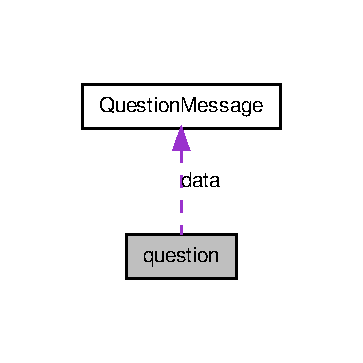
\includegraphics[width=174pt]{structquestion__coll__graph}
\end{center}
\end{figure}
\subsection*{Data Fields}
\begin{DoxyCompactItemize}
\item 
const uint8\_\-t \hyperlink{structquestion_aca7dafb0092715a03dd40f45fc607f2a}{type}
\item 
uint16\_\-t \hyperlink{structquestion_a1892eba2086d12ac2b09005aeb09ea3b}{length}
\item 
\hyperlink{struct_question_message}{QuestionMessage} \hyperlink{structquestion_a17a102c002c052d9c66ef8eee24429d7}{data}
\end{DoxyCompactItemize}


\subsection{Field Documentation}
\hypertarget{structquestion_a17a102c002c052d9c66ef8eee24429d7}{
\index{question@{question}!data@{data}}
\index{data@{data}!question@{question}}
\subsubsection[{data}]{\setlength{\rightskip}{0pt plus 5cm}{\bf QuestionMessage} {\bf data}}}
\label{structquestion_a17a102c002c052d9c66ef8eee24429d7}
\hypertarget{structquestion_a1892eba2086d12ac2b09005aeb09ea3b}{
\index{question@{question}!length@{length}}
\index{length@{length}!question@{question}}
\subsubsection[{length}]{\setlength{\rightskip}{0pt plus 5cm}uint16\_\-t {\bf length}}}
\label{structquestion_a1892eba2086d12ac2b09005aeb09ea3b}
\hypertarget{structquestion_aca7dafb0092715a03dd40f45fc607f2a}{
\index{question@{question}!type@{type}}
\index{type@{type}!question@{question}}
\subsubsection[{type}]{\setlength{\rightskip}{0pt plus 5cm}const uint8\_\-t {\bf type}}}
\label{structquestion_aca7dafb0092715a03dd40f45fc607f2a}


The documentation for this struct was generated from the following file:\begin{DoxyCompactItemize}
\item 
/home/kathrin/Documents/fh/sysprog/YDKR/source/common/src/\hyperlink{messages_8h}{messages.h}\end{DoxyCompactItemize}

\hypertarget{structquestion__answered}{
\section{question\_\-answered Struct Reference}
\label{structquestion__answered}\index{question\_\-answered@{question\_\-answered}}
}


{\ttfamily \#include $<$messages.h$>$}

\subsection*{Data Fields}
\begin{DoxyCompactItemize}
\item 
const uint8\_\-t \hyperlink{structquestion__answered_aca7dafb0092715a03dd40f45fc607f2a}{type}
\item 
uint16\_\-t \hyperlink{structquestion__answered_a1892eba2086d12ac2b09005aeb09ea3b}{length}
\item 
uint8\_\-t \hyperlink{structquestion__answered_af190e8c7f8c6caf004f782b3aa7b5021}{selection}
\end{DoxyCompactItemize}


\subsection{Field Documentation}
\hypertarget{structquestion__answered_a1892eba2086d12ac2b09005aeb09ea3b}{
\index{question\_\-answered@{question\_\-answered}!length@{length}}
\index{length@{length}!question_answered@{question\_\-answered}}
\subsubsection[{length}]{\setlength{\rightskip}{0pt plus 5cm}uint16\_\-t {\bf length}}}
\label{structquestion__answered_a1892eba2086d12ac2b09005aeb09ea3b}
\hypertarget{structquestion__answered_af190e8c7f8c6caf004f782b3aa7b5021}{
\index{question\_\-answered@{question\_\-answered}!selection@{selection}}
\index{selection@{selection}!question_answered@{question\_\-answered}}
\subsubsection[{selection}]{\setlength{\rightskip}{0pt plus 5cm}uint8\_\-t {\bf selection}}}
\label{structquestion__answered_af190e8c7f8c6caf004f782b3aa7b5021}
\hypertarget{structquestion__answered_aca7dafb0092715a03dd40f45fc607f2a}{
\index{question\_\-answered@{question\_\-answered}!type@{type}}
\index{type@{type}!question_answered@{question\_\-answered}}
\subsubsection[{type}]{\setlength{\rightskip}{0pt plus 5cm}const uint8\_\-t {\bf type}}}
\label{structquestion__answered_aca7dafb0092715a03dd40f45fc607f2a}


The documentation for this struct was generated from the following file:\begin{DoxyCompactItemize}
\item 
/home/kathrin/Documents/fh/sysprog/YDKR/source/common/src/\hyperlink{messages_8h}{messages.h}\end{DoxyCompactItemize}

\hypertarget{structquestion__request}{
\section{question\_\-request Struct Reference}
\label{structquestion__request}\index{question\_\-request@{question\_\-request}}
}


{\ttfamily \#include $<$messages.h$>$}

\subsection*{Data Fields}
\begin{DoxyCompactItemize}
\item 
const uint8\_\-t \hyperlink{structquestion__request_aca7dafb0092715a03dd40f45fc607f2a}{type}
\item 
uint16\_\-t \hyperlink{structquestion__request_a1892eba2086d12ac2b09005aeb09ea3b}{length}
\end{DoxyCompactItemize}


\subsection{Field Documentation}
\hypertarget{structquestion__request_a1892eba2086d12ac2b09005aeb09ea3b}{
\index{question\_\-request@{question\_\-request}!length@{length}}
\index{length@{length}!question_request@{question\_\-request}}
\subsubsection[{length}]{\setlength{\rightskip}{0pt plus 5cm}uint16\_\-t {\bf length}}}
\label{structquestion__request_a1892eba2086d12ac2b09005aeb09ea3b}
\hypertarget{structquestion__request_aca7dafb0092715a03dd40f45fc607f2a}{
\index{question\_\-request@{question\_\-request}!type@{type}}
\index{type@{type}!question_request@{question\_\-request}}
\subsubsection[{type}]{\setlength{\rightskip}{0pt plus 5cm}const uint8\_\-t {\bf type}}}
\label{structquestion__request_aca7dafb0092715a03dd40f45fc607f2a}


The documentation for this struct was generated from the following file:\begin{DoxyCompactItemize}
\item 
/home/kathrin/Documents/fh/sysprog/YDKR/source/common/src/\hyperlink{messages_8h}{messages.h}\end{DoxyCompactItemize}

\hypertarget{structquestion__result}{
\section{question\_\-result Struct Reference}
\label{structquestion__result}\index{question\_\-result@{question\_\-result}}
}


{\ttfamily \#include $<$messages.h$>$}

\subsection*{Data Fields}
\begin{DoxyCompactItemize}
\item 
const uint8\_\-t \hyperlink{structquestion__result_aca7dafb0092715a03dd40f45fc607f2a}{type}
\item 
uint16\_\-t \hyperlink{structquestion__result_a1892eba2086d12ac2b09005aeb09ea3b}{length}
\item 
uint8\_\-t \hyperlink{structquestion__result_af190e8c7f8c6caf004f782b3aa7b5021}{selection}
\item 
uint8\_\-t \hyperlink{structquestion__result_a9e77be6b2d809446ab999d825cfb84f3}{correct}
\end{DoxyCompactItemize}


\subsection{Field Documentation}
\hypertarget{structquestion__result_a9e77be6b2d809446ab999d825cfb84f3}{
\index{question\_\-result@{question\_\-result}!correct@{correct}}
\index{correct@{correct}!question_result@{question\_\-result}}
\subsubsection[{correct}]{\setlength{\rightskip}{0pt plus 5cm}uint8\_\-t {\bf correct}}}
\label{structquestion__result_a9e77be6b2d809446ab999d825cfb84f3}
\hypertarget{structquestion__result_a1892eba2086d12ac2b09005aeb09ea3b}{
\index{question\_\-result@{question\_\-result}!length@{length}}
\index{length@{length}!question_result@{question\_\-result}}
\subsubsection[{length}]{\setlength{\rightskip}{0pt plus 5cm}uint16\_\-t {\bf length}}}
\label{structquestion__result_a1892eba2086d12ac2b09005aeb09ea3b}
\hypertarget{structquestion__result_af190e8c7f8c6caf004f782b3aa7b5021}{
\index{question\_\-result@{question\_\-result}!selection@{selection}}
\index{selection@{selection}!question_result@{question\_\-result}}
\subsubsection[{selection}]{\setlength{\rightskip}{0pt plus 5cm}uint8\_\-t {\bf selection}}}
\label{structquestion__result_af190e8c7f8c6caf004f782b3aa7b5021}
\hypertarget{structquestion__result_aca7dafb0092715a03dd40f45fc607f2a}{
\index{question\_\-result@{question\_\-result}!type@{type}}
\index{type@{type}!question_result@{question\_\-result}}
\subsubsection[{type}]{\setlength{\rightskip}{0pt plus 5cm}const uint8\_\-t {\bf type}}}
\label{structquestion__result_aca7dafb0092715a03dd40f45fc607f2a}


The documentation for this struct was generated from the following file:\begin{DoxyCompactItemize}
\item 
/home/kathrin/Documents/fh/sysprog/YDKR/source/common/src/\hyperlink{messages_8h}{messages.h}\end{DoxyCompactItemize}

\hypertarget{struct_question_message}{
\section{QuestionMessage Struct Reference}
\label{struct_question_message}\index{QuestionMessage@{QuestionMessage}}
}


Darstellung einer Frage während des Transports zum Client.  




{\ttfamily \#include $<$question.h$>$}

\subsection*{Data Fields}
\begin{DoxyCompactItemize}
\item 
char \hyperlink{struct_question_message_a4b07688ced7937f6eb270f34c6870281}{question} \mbox{[}QUESTION\_\-SIZE\mbox{]}
\item 
char \hyperlink{struct_question_message_aee7134a1e311755686d480c3f8b963c7}{answers} \mbox{[}NUM\_\-ANSWERS\mbox{]}\mbox{[}ANSWER\_\-SIZE\mbox{]}
\item 
uint16\_\-t \hyperlink{struct_question_message_a7f1ad43d3bf79b40bc39dbb5a6c3a5ae}{timeout}
\end{DoxyCompactItemize}


\subsection{Detailed Description}
Darstellung einer Frage während des Transports zum Client. \begin{DoxyAttention}{Attention}
Muss bis auf das Fehlen der Variable correct exakt gleich sein wie die Question-\/Struktur 
\end{DoxyAttention}


\subsection{Field Documentation}
\hypertarget{struct_question_message_aee7134a1e311755686d480c3f8b963c7}{
\index{QuestionMessage@{QuestionMessage}!answers@{answers}}
\index{answers@{answers}!QuestionMessage@{QuestionMessage}}
\subsubsection[{answers}]{\setlength{\rightskip}{0pt plus 5cm}char {\bf answers}\mbox{[}NUM\_\-ANSWERS\mbox{]}\mbox{[}ANSWER\_\-SIZE\mbox{]}}}
\label{struct_question_message_aee7134a1e311755686d480c3f8b963c7}
Antworten \hypertarget{struct_question_message_a4b07688ced7937f6eb270f34c6870281}{
\index{QuestionMessage@{QuestionMessage}!question@{question}}
\index{question@{question}!QuestionMessage@{QuestionMessage}}
\subsubsection[{question}]{\setlength{\rightskip}{0pt plus 5cm}char {\bf question}\mbox{[}QUESTION\_\-SIZE\mbox{]}}}
\label{struct_question_message_a4b07688ced7937f6eb270f34c6870281}
Text der Fragestellung \hypertarget{struct_question_message_a7f1ad43d3bf79b40bc39dbb5a6c3a5ae}{
\index{QuestionMessage@{QuestionMessage}!timeout@{timeout}}
\index{timeout@{timeout}!QuestionMessage@{QuestionMessage}}
\subsubsection[{timeout}]{\setlength{\rightskip}{0pt plus 5cm}uint16\_\-t {\bf timeout}}}
\label{struct_question_message_a7f1ad43d3bf79b40bc39dbb5a6c3a5ae}
Zeit für diese Frage in Sekunden (zu Informationszwecken mitgesendet) 

The documentation for this struct was generated from the following file:\begin{DoxyCompactItemize}
\item 
/home/kathrin/Documents/fh/sysprog/YDKR/source/common/src/\hyperlink{question_8h}{question.h}\end{DoxyCompactItemize}

\hypertarget{structquestion_result}{
\section{questionResult Struct Reference}
\label{structquestion_result}\index{questionResult@{questionResult}}
}


{\ttfamily \#include $<$listener.h$>$}

\subsection*{Data Fields}
\begin{DoxyCompactItemize}
\item 
uint8\_\-t \hyperlink{structquestion_result_af190e8c7f8c6caf004f782b3aa7b5021}{selection}
\item 
uint8\_\-t \hyperlink{structquestion_result_a9e77be6b2d809446ab999d825cfb84f3}{correct}
\end{DoxyCompactItemize}


\subsection{Field Documentation}
\hypertarget{structquestion_result_a9e77be6b2d809446ab999d825cfb84f3}{
\index{questionResult@{questionResult}!correct@{correct}}
\index{correct@{correct}!questionResult@{questionResult}}
\subsubsection[{correct}]{\setlength{\rightskip}{0pt plus 5cm}uint8\_\-t {\bf correct}}}
\label{structquestion_result_a9e77be6b2d809446ab999d825cfb84f3}
\hypertarget{structquestion_result_af190e8c7f8c6caf004f782b3aa7b5021}{
\index{questionResult@{questionResult}!selection@{selection}}
\index{selection@{selection}!questionResult@{questionResult}}
\subsubsection[{selection}]{\setlength{\rightskip}{0pt plus 5cm}uint8\_\-t {\bf selection}}}
\label{structquestion_result_af190e8c7f8c6caf004f782b3aa7b5021}


The documentation for this struct was generated from the following file:\begin{DoxyCompactItemize}
\item 
/home/kathrin/Documents/fh/sysprog/YDKR/source/client/src/\hyperlink{listener_8h}{listener.h}\end{DoxyCompactItemize}

\hypertarget{structstart__game}{
\section{start\_\-game Struct Reference}
\label{structstart__game}\index{start\_\-game@{start\_\-game}}
}


{\ttfamily \#include $<$messages.h$>$}

\subsection*{Data Fields}
\begin{DoxyCompactItemize}
\item 
const uint8\_\-t \hyperlink{structstart__game_aca7dafb0092715a03dd40f45fc607f2a}{type}
\item 
uint16\_\-t \hyperlink{structstart__game_a1892eba2086d12ac2b09005aeb09ea3b}{length}
\item 
char $\ast$ \hyperlink{structstart__game_aeac90097f29f7529968697163cea5c18}{filename}
\end{DoxyCompactItemize}


\subsection{Field Documentation}
\hypertarget{structstart__game_aeac90097f29f7529968697163cea5c18}{
\index{start\_\-game@{start\_\-game}!filename@{filename}}
\index{filename@{filename}!start_game@{start\_\-game}}
\subsubsection[{filename}]{\setlength{\rightskip}{0pt plus 5cm}char$\ast$ {\bf filename}}}
\label{structstart__game_aeac90097f29f7529968697163cea5c18}
\hypertarget{structstart__game_a1892eba2086d12ac2b09005aeb09ea3b}{
\index{start\_\-game@{start\_\-game}!length@{length}}
\index{length@{length}!start_game@{start\_\-game}}
\subsubsection[{length}]{\setlength{\rightskip}{0pt plus 5cm}uint16\_\-t {\bf length}}}
\label{structstart__game_a1892eba2086d12ac2b09005aeb09ea3b}
\hypertarget{structstart__game_aca7dafb0092715a03dd40f45fc607f2a}{
\index{start\_\-game@{start\_\-game}!type@{type}}
\index{type@{type}!start_game@{start\_\-game}}
\subsubsection[{type}]{\setlength{\rightskip}{0pt plus 5cm}const uint8\_\-t {\bf type}}}
\label{structstart__game_aca7dafb0092715a03dd40f45fc607f2a}


The documentation for this struct was generated from the following file:\begin{DoxyCompactItemize}
\item 
/home/kathrin/Documents/fh/sysprog/YDKR/source/common/src/\hyperlink{messages_8h}{messages.h}\end{DoxyCompactItemize}

\chapter{File Documentation}
\hypertarget{client_8c}{
\section{/home/kathrin/Documents/fh/sysprog/YDKR/source/client/src/client.c File Reference}
\label{client_8c}\index{/home/kathrin/Documents/fh/sysprog/YDKR/source/client/src/client.c@{/home/kathrin/Documents/fh/sysprog/YDKR/source/client/src/client.c}}
}
{\ttfamily \#include $<$stdio.h$>$}\par
{\ttfamily \#include $<$stdlib.h$>$}\par
{\ttfamily \#include $<$string.h$>$}\par
{\ttfamily \#include $<$sys/time.h$>$}\par
{\ttfamily \#include $<$sys/types.h$>$}\par
{\ttfamily \#include $<$unistd.h$>$}\par
{\ttfamily \#include $<$sys/socket.h$>$}\par
{\ttfamily \#include $<$netdb.h$>$}\par
{\ttfamily \#include $<$netinet/in.h$>$}\par
{\ttfamily \#include $<$arpa/inet.h$>$}\par
{\ttfamily \#include $<$getopt.h$>$}\par
{\ttfamily \#include \char`\"{}gui\_\-interface.h\char`\"{}}\par
{\ttfamily \#include \char`\"{}client.h\char`\"{}}\par
{\ttfamily \#include \char`\"{}fragewechsel.h\char`\"{}}\par
{\ttfamily \#include \char`\"{}listener.h\char`\"{}}\par
Include dependency graph for client.c:
\nopagebreak
\begin{figure}[H]
\begin{center}
\leavevmode
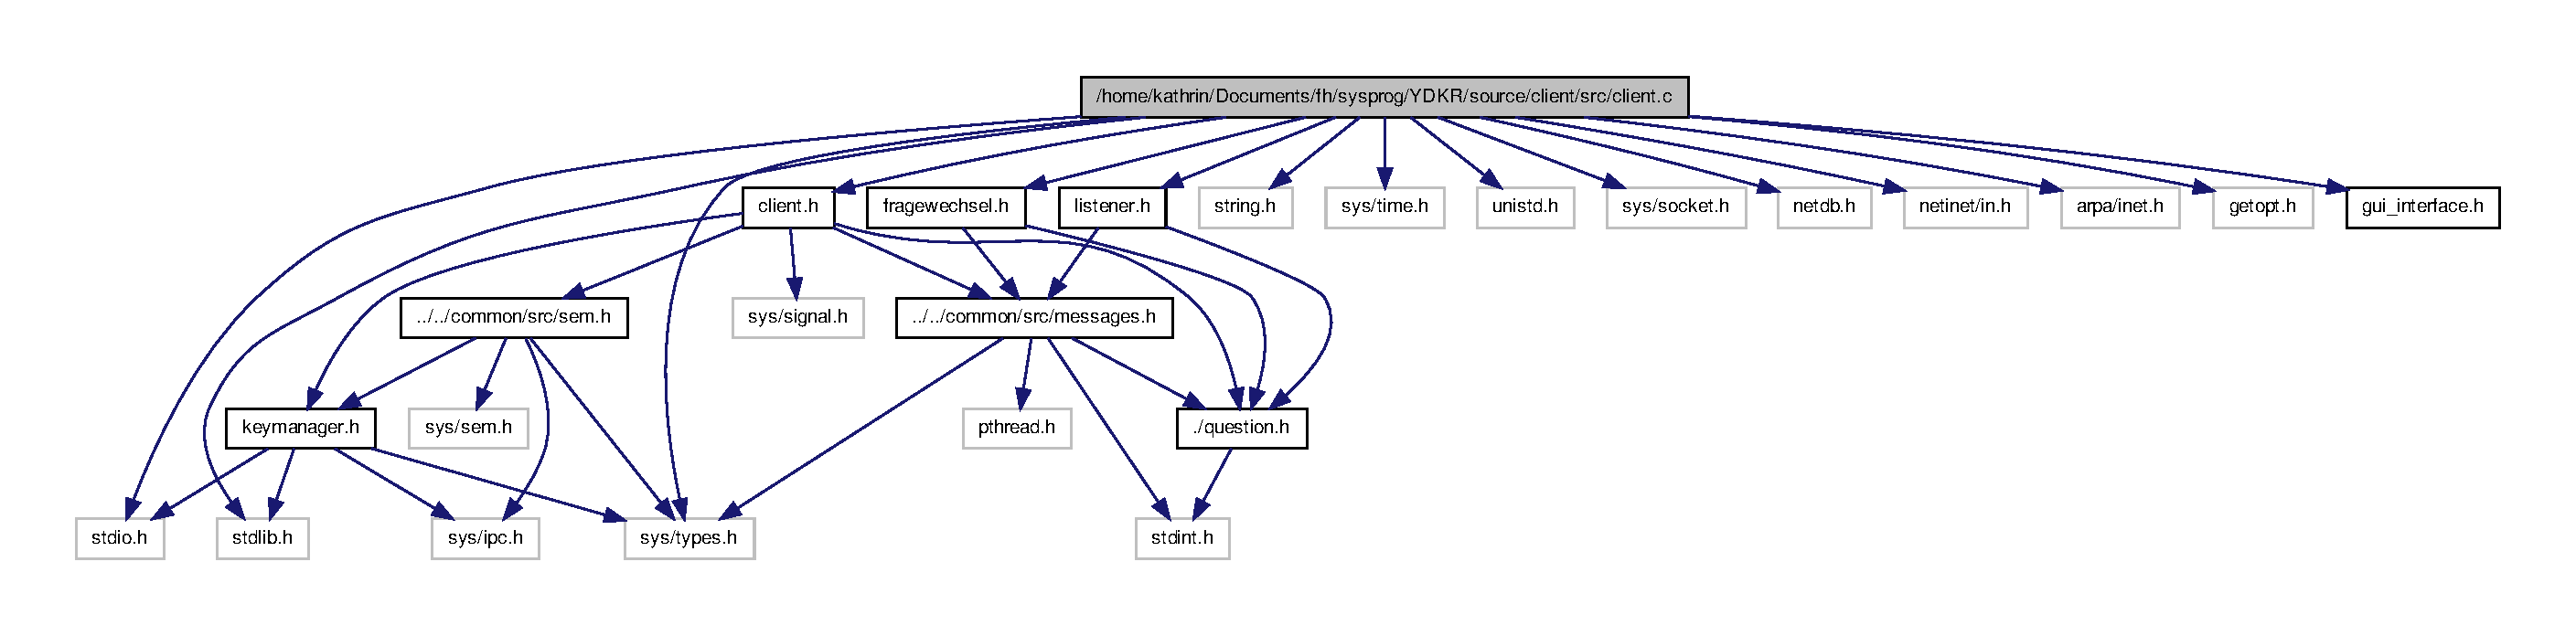
\includegraphics[width=400pt]{client_8c__incl}
\end{center}
\end{figure}
\subsection*{Functions}
\begin{DoxyCompactItemize}
\item 
void \hyperlink{client_8c_ac594e87e65b86745d13a211ded7339d8}{print\_\-help} (char $\ast$self)
\begin{DoxyCompactList}\small\item\em prints the help instructions \item\end{DoxyCompactList}\item 
int \hyperlink{client_8c_a3c04138a5bfe5d72780bb7e82a18e627}{main} (int argc, char $\ast$$\ast$argv)
\begin{DoxyCompactList}\small\item\em main thread, starting up the client and the other threads \item\end{DoxyCompactList}\item 
void \hyperlink{client_8c_a544b7ea288ff725efa662ceb07fa14ce}{send\_\-login} (char $\ast$name)
\item 
int \hyperlink{client_8c_a3ff77331b6c7b11926e9ba2185bb3514}{wait\_\-loginOK} ()
\begin{DoxyCompactList}\small\item\em waits until login response from server is ok -\/-\/-\/-\/-\/-\/-\/-\/-\/-\/-\/-\/-\/-\/-\/-\/-\/-\/-\/-\/-\/-\/-\/-\/-\/-\/-\/-\/-\/-\/-\/-\/-\/-\/-\/-\/-\/-\/-\/-\/-\/-\/-\/-\/-\/-\/-\/-\/-\/-\/-\/-\/-\/-\/-\/-\/-\/-\/-\/ \item\end{DoxyCompactList}\item 
void \hyperlink{client_8c_a8eb72d0038a8d927d73051979d247852}{setClientMode} ()
\begin{DoxyCompactList}\small\item\em sets the Client Mode to privileged or normal -\/-\/-\/-\/-\/-\/-\/-\/-\/-\/-\/-\/-\/-\/-\/-\/-\/-\/-\/-\/-\/-\/-\/-\/-\/-\/-\/-\/-\/-\/-\/-\/-\/-\/-\/-\/-\/-\/-\/-\/-\/-\/-\/-\/-\/-\/-\/-\/-\/-\/-\/-\/-\/-\/-\/-\/-\/-\/-\/ \item\end{DoxyCompactList}\item 
void \hyperlink{client_8c_aad8abca9f1cd7f320ff47cbc339e7ce6}{sendCR} ()
\begin{DoxyCompactList}\small\item\em sends the Catalouge Request -\/-\/-\/-\/-\/-\/-\/-\/-\/-\/-\/-\/-\/-\/-\/-\/-\/-\/-\/-\/-\/-\/-\/-\/-\/-\/-\/-\/-\/-\/-\/-\/-\/-\/-\/-\/-\/-\/-\/-\/-\/-\/-\/-\/-\/-\/-\/-\/-\/-\/-\/-\/-\/-\/-\/-\/-\/-\/-\/ \item\end{DoxyCompactList}\item 
void \hyperlink{client_8c_af5fa27f55f83b974722c008df85bc723}{send\_\-QR} (int sleepTime)
\begin{DoxyCompactList}\small\item\em sends question request to the server after a special waiting time. =========================================================================== \item\end{DoxyCompactList}\item 
void \hyperlink{client_8c_a258e3b580e688a0cf46e4258525aeaf1}{sigint\_\-handler} (int sig)
\begin{DoxyCompactList}\small\item\em cleaning up function \item\end{DoxyCompactList}\end{DoxyCompactItemize}
\subsection*{Variables}
\begin{DoxyCompactItemize}
\item 
pthread\_\-t \hyperlink{client_8c_a72379812c6fc31ef5e5520084b5a7ee3}{listener\_\-thread\_\-id}
\item 
pthread\_\-t \hyperlink{client_8c_a6748da5abcf80456846d3fc37e4fb2b6}{fragen\_\-thread\_\-id}
\end{DoxyCompactItemize}


\subsection{Detailed Description}
============================================================================

\begin{DoxyAuthor}{Author}
: Kathrin Holzmann 
\end{DoxyAuthor}
\begin{DoxyDate}{Date}
: Apr 12, 2011 ============================================================================
\end{DoxyDate}
============================================================================

\begin{DoxyAuthor}{Author}
: Kathrin Holzmann 
\end{DoxyAuthor}
\begin{DoxyDate}{Date}
: May 12, 2011 ============================================================================ 
\end{DoxyDate}


\subsection{Function Documentation}
\hypertarget{client_8c_a3c04138a5bfe5d72780bb7e82a18e627}{
\index{client.c@{client.c}!main@{main}}
\index{main@{main}!client.c@{client.c}}
\subsubsection[{main}]{\setlength{\rightskip}{0pt plus 5cm}int main (
\begin{DoxyParamCaption}
\item[{int}]{argc, }
\item[{char $\ast$$\ast$}]{argv}
\end{DoxyParamCaption}
)}}
\label{client_8c_a3c04138a5bfe5d72780bb7e82a18e627}


main thread, starting up the client and the other threads 

=========================================== 
\begin{DoxyParams}{Parameters}
{\em argc:int} & argv$\ast$$\ast$char ========================================== \\
\hline
\end{DoxyParams}
\hypertarget{client_8c_ac594e87e65b86745d13a211ded7339d8}{
\index{client.c@{client.c}!print\_\-help@{print\_\-help}}
\index{print\_\-help@{print\_\-help}!client.c@{client.c}}
\subsubsection[{print\_\-help}]{\setlength{\rightskip}{0pt plus 5cm}void print\_\-help (
\begin{DoxyParamCaption}
\item[{char $\ast$}]{self}
\end{DoxyParamCaption}
)}}
\label{client_8c_ac594e87e65b86745d13a211ded7339d8}


prints the help instructions 

======================================== 
\begin{DoxyParams}{Parameters}
{\em self} & $\ast$char ======================================= \\
\hline
\end{DoxyParams}
\hypertarget{client_8c_a544b7ea288ff725efa662ceb07fa14ce}{
\index{client.c@{client.c}!send\_\-login@{send\_\-login}}
\index{send\_\-login@{send\_\-login}!client.c@{client.c}}
\subsubsection[{send\_\-login}]{\setlength{\rightskip}{0pt plus 5cm}void send\_\-login (
\begin{DoxyParamCaption}
\item[{char $\ast$}]{name}
\end{DoxyParamCaption}
)}}
\label{client_8c_a544b7ea288ff725efa662ceb07fa14ce}
-\/-\/-\/-\/-\/-\/-\/-\/-\/-\/-\/void \hyperlink{client_2src_2client_8h_a544b7ea288ff725efa662ceb07fa14ce}{send\_\-login(char$\ast$ name)}-\/-\/-\/-\/-\/-\/-\/-\/-\/-\/-\/-\/-\/-\/-\/-\/-\/-\/-\/-\/-\/-\/ : sends the login name to the server -\/-\/-\/-\/-\/-\/-\/-\/-\/-\/-\/-\/-\/-\/-\/-\/-\/-\/-\/-\/-\/-\/-\/-\/-\/-\/-\/-\/-\/-\/-\/-\/-\/-\/-\/-\/-\/-\/-\/-\/-\/-\/-\/-\/-\/-\/-\/-\/-\/-\/-\/-\/-\/-\/-\/-\/-\/-\/-\/ \hypertarget{client_8c_af5fa27f55f83b974722c008df85bc723}{
\index{client.c@{client.c}!send\_\-QR@{send\_\-QR}}
\index{send\_\-QR@{send\_\-QR}!client.c@{client.c}}
\subsubsection[{send\_\-QR}]{\setlength{\rightskip}{0pt plus 5cm}void send\_\-QR (
\begin{DoxyParamCaption}
\item[{int}]{sleepTime}
\end{DoxyParamCaption}
)}}
\label{client_8c_af5fa27f55f83b974722c008df85bc723}


sends question request to the server after a special waiting time. =========================================================================== 

========================================================================== \hypertarget{client_8c_aad8abca9f1cd7f320ff47cbc339e7ce6}{
\index{client.c@{client.c}!sendCR@{sendCR}}
\index{sendCR@{sendCR}!client.c@{client.c}}
\subsubsection[{sendCR}]{\setlength{\rightskip}{0pt plus 5cm}void sendCR (
\begin{DoxyParamCaption}
{}
\end{DoxyParamCaption}
)}}
\label{client_8c_aad8abca9f1cd7f320ff47cbc339e7ce6}


sends the Catalouge Request -\/-\/-\/-\/-\/-\/-\/-\/-\/-\/-\/-\/-\/-\/-\/-\/-\/-\/-\/-\/-\/-\/-\/-\/-\/-\/-\/-\/-\/-\/-\/-\/-\/-\/-\/-\/-\/-\/-\/-\/-\/-\/-\/-\/-\/-\/-\/-\/-\/-\/-\/-\/-\/-\/-\/-\/-\/-\/-\/ 

-\/-\/-\/-\/-\/-\/-\/-\/-\/-\/-\/void \hyperlink{client_8c_aad8abca9f1cd7f320ff47cbc339e7ce6}{sendCR()}-\/-\/-\/-\/-\/-\/-\/-\/-\/-\/-\/-\/-\/-\/-\/-\/-\/-\/-\/-\/-\/-\/-\/-\/-\/-\/-\/-\/-\/-\/-\/-\/-\/ \hypertarget{client_8c_a8eb72d0038a8d927d73051979d247852}{
\index{client.c@{client.c}!setClientMode@{setClientMode}}
\index{setClientMode@{setClientMode}!client.c@{client.c}}
\subsubsection[{setClientMode}]{\setlength{\rightskip}{0pt plus 5cm}void setClientMode (
\begin{DoxyParamCaption}
{}
\end{DoxyParamCaption}
)}}
\label{client_8c_a8eb72d0038a8d927d73051979d247852}


sets the Client Mode to privileged or normal -\/-\/-\/-\/-\/-\/-\/-\/-\/-\/-\/-\/-\/-\/-\/-\/-\/-\/-\/-\/-\/-\/-\/-\/-\/-\/-\/-\/-\/-\/-\/-\/-\/-\/-\/-\/-\/-\/-\/-\/-\/-\/-\/-\/-\/-\/-\/-\/-\/-\/-\/-\/-\/-\/-\/-\/-\/-\/-\/ 

-\/-\/-\/-\/-\/-\/-\/-\/-\/-\/-\/void \hyperlink{client_8c_a8eb72d0038a8d927d73051979d247852}{setClientMode()}-\/-\/-\/-\/-\/-\/-\/-\/-\/-\/-\/-\/-\/-\/-\/-\/-\/-\/-\/-\/-\/-\/-\/-\/-\/-\/-\/ \hypertarget{client_8c_a258e3b580e688a0cf46e4258525aeaf1}{
\index{client.c@{client.c}!sigint\_\-handler@{sigint\_\-handler}}
\index{sigint\_\-handler@{sigint\_\-handler}!client.c@{client.c}}
\subsubsection[{sigint\_\-handler}]{\setlength{\rightskip}{0pt plus 5cm}void sigint\_\-handler (
\begin{DoxyParamCaption}
\item[{int}]{sig}
\end{DoxyParamCaption}
)}}
\label{client_8c_a258e3b580e688a0cf46e4258525aeaf1}


cleaning up function 

========================================== 
\begin{DoxyParams}{Parameters}
{\em signal:INT} & ============================================ \\
\hline
\end{DoxyParams}
\hypertarget{client_8c_a3ff77331b6c7b11926e9ba2185bb3514}{
\index{client.c@{client.c}!wait\_\-loginOK@{wait\_\-loginOK}}
\index{wait\_\-loginOK@{wait\_\-loginOK}!client.c@{client.c}}
\subsubsection[{wait\_\-loginOK}]{\setlength{\rightskip}{0pt plus 5cm}int wait\_\-loginOK (
\begin{DoxyParamCaption}
{}
\end{DoxyParamCaption}
)}}
\label{client_8c_a3ff77331b6c7b11926e9ba2185bb3514}


waits until login response from server is ok -\/-\/-\/-\/-\/-\/-\/-\/-\/-\/-\/-\/-\/-\/-\/-\/-\/-\/-\/-\/-\/-\/-\/-\/-\/-\/-\/-\/-\/-\/-\/-\/-\/-\/-\/-\/-\/-\/-\/-\/-\/-\/-\/-\/-\/-\/-\/-\/-\/-\/-\/-\/-\/-\/-\/-\/-\/-\/-\/ 

-\/-\/-\/-\/-\/-\/-\/-\/-\/-\/-\/int wat\_\-loginOK()-\/-\/-\/-\/-\/-\/-\/-\/-\/-\/-\/-\/-\/-\/-\/-\/-\/-\/-\/-\/-\/-\/-\/-\/-\/-\/-\/ 

\subsection{Variable Documentation}
\hypertarget{client_8c_a6748da5abcf80456846d3fc37e4fb2b6}{
\index{client.c@{client.c}!fragen\_\-thread\_\-id@{fragen\_\-thread\_\-id}}
\index{fragen\_\-thread\_\-id@{fragen\_\-thread\_\-id}!client.c@{client.c}}
\subsubsection[{fragen\_\-thread\_\-id}]{\setlength{\rightskip}{0pt plus 5cm}pthread\_\-t {\bf fragen\_\-thread\_\-id}}}
\label{client_8c_a6748da5abcf80456846d3fc37e4fb2b6}
\hypertarget{client_8c_a72379812c6fc31ef5e5520084b5a7ee3}{
\index{client.c@{client.c}!listener\_\-thread\_\-id@{listener\_\-thread\_\-id}}
\index{listener\_\-thread\_\-id@{listener\_\-thread\_\-id}!client.c@{client.c}}
\subsubsection[{listener\_\-thread\_\-id}]{\setlength{\rightskip}{0pt plus 5cm}pthread\_\-t {\bf listener\_\-thread\_\-id}}}
\label{client_8c_a72379812c6fc31ef5e5520084b5a7ee3}

\hypertarget{client_2src_2client_8h}{
\section{/home/kathrin/Documents/fh/sysprog/YDKR/source/client/src/client.h File Reference}
\label{client_2src_2client_8h}\index{/home/kathrin/Documents/fh/sysprog/YDKR/source/client/src/client.h@{/home/kathrin/Documents/fh/sysprog/YDKR/source/client/src/client.h}}
}
{\ttfamily \#include \char`\"{}../../common/src/messages.h\char`\"{}}\par
{\ttfamily \#include \char`\"{}../../common/src/question.h\char`\"{}}\par
{\ttfamily \#include \char`\"{}../../common/src/sem.h\char`\"{}}\par
{\ttfamily \#include \char`\"{}../../common/src/keymanager.h\char`\"{}}\par
{\ttfamily \#include $<$sys/signal.h$>$}\par
Include dependency graph for client.h:
\nopagebreak
\begin{figure}[H]
\begin{center}
\leavevmode
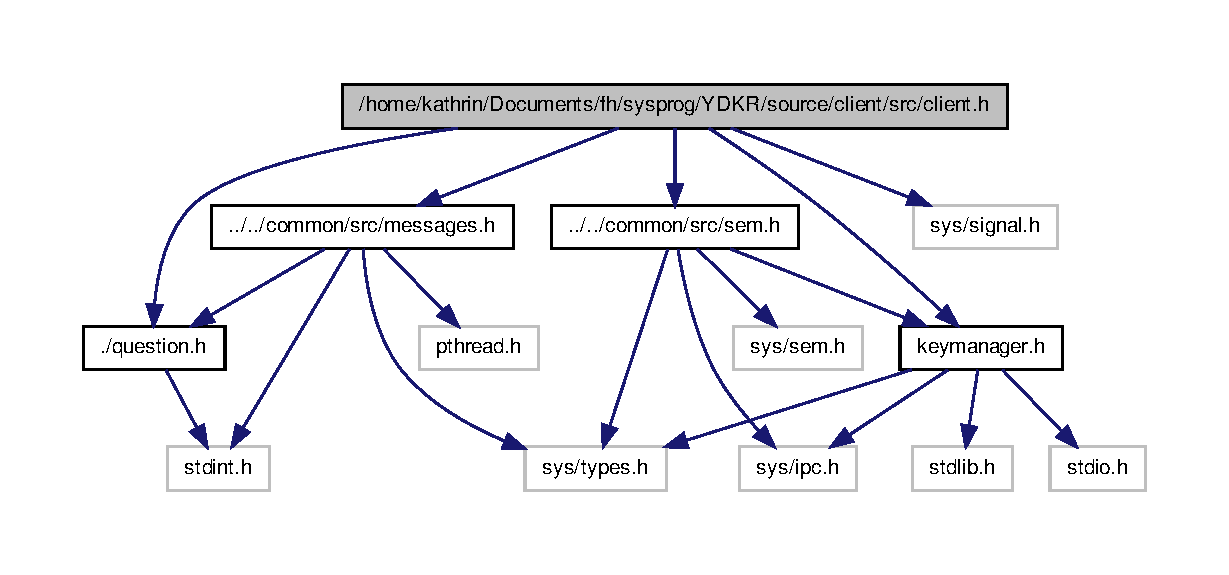
\includegraphics[width=400pt]{client_2src_2client_8h__incl}
\end{center}
\end{figure}
This graph shows which files directly or indirectly include this file:
\nopagebreak
\begin{figure}[H]
\begin{center}
\leavevmode
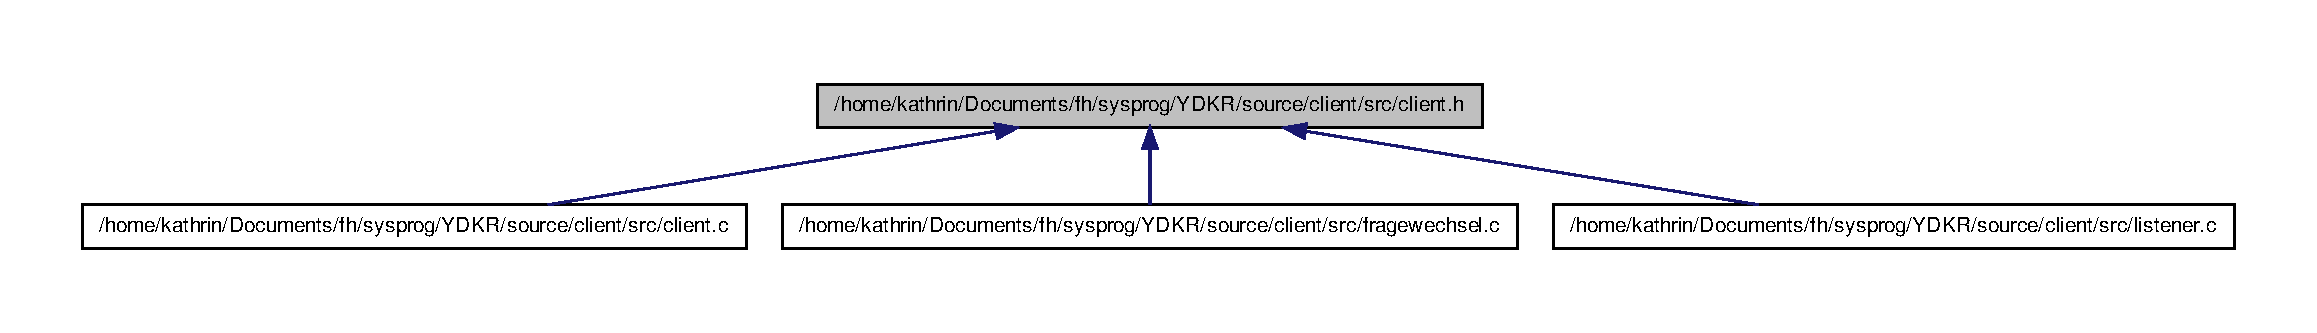
\includegraphics[width=400pt]{client_2src_2client_8h__dep__incl}
\end{center}
\end{figure}
\subsection*{Data Structures}
\begin{DoxyCompactItemize}
\item 
struct \hyperlink{structglobal__client__info}{global\_\-client\_\-info}
\item 
struct \hyperlink{structerror_m_s_g}{errorMSG}
\end{DoxyCompactItemize}
\subsection*{Defines}
\begin{DoxyCompactItemize}
\item 
\#define \hyperlink{client_2src_2client_8h_ad8f2a644dcd54e9e4a3678d899a5a4f7}{ERR\_\-OOM}~-\/1
\item 
\#define \hyperlink{client_2src_2client_8h_a87e9272b1fcf0daa57b86fafcb90c0fe}{ERR\_\-KILL\_\-CLIENT}~-\/2
\end{DoxyCompactItemize}
\subsection*{Enumerations}
\begin{DoxyCompactItemize}
\item 
enum \hyperlink{client_2src_2client_8h_a12ca651cd1b9eb7aeeb0d0c8a2cdd5e0}{gameStatus} \{ \hyperlink{client_2src_2client_8h_a12ca651cd1b9eb7aeeb0d0c8a2cdd5e0a482c39b4341ccf2ef0f91f784d67f8c8}{preparation}, 
\hyperlink{client_2src_2client_8h_a12ca651cd1b9eb7aeeb0d0c8a2cdd5e0a593fcb971576d8ee918ec9eaad2678d6}{playing}, 
\hyperlink{client_2src_2client_8h_a12ca651cd1b9eb7aeeb0d0c8a2cdd5e0a80b1a820e533d7cf0e1715319339e6d0}{end}
 \}
\end{DoxyCompactItemize}
\subsection*{Functions}
\begin{DoxyCompactItemize}
\item 
void \hyperlink{client_2src_2client_8h_a544b7ea288ff725efa662ceb07fa14ce}{send\_\-login} (char $\ast$name)
\item 
int \hyperlink{client_2src_2client_8h_a3ff77331b6c7b11926e9ba2185bb3514}{wait\_\-loginOK} ()
\begin{DoxyCompactList}\small\item\em waits until login response from server is ok -\/-\/-\/-\/-\/-\/-\/-\/-\/-\/-\/-\/-\/-\/-\/-\/-\/-\/-\/-\/-\/-\/-\/-\/-\/-\/-\/-\/-\/-\/-\/-\/-\/-\/-\/-\/-\/-\/-\/-\/-\/-\/-\/-\/-\/-\/-\/-\/-\/-\/-\/-\/-\/-\/-\/-\/-\/-\/-\/ \item\end{DoxyCompactList}\item 
void \hyperlink{client_2src_2client_8h_a8eb72d0038a8d927d73051979d247852}{setClientMode} ()
\begin{DoxyCompactList}\small\item\em sets the Client Mode to privileged or normal -\/-\/-\/-\/-\/-\/-\/-\/-\/-\/-\/-\/-\/-\/-\/-\/-\/-\/-\/-\/-\/-\/-\/-\/-\/-\/-\/-\/-\/-\/-\/-\/-\/-\/-\/-\/-\/-\/-\/-\/-\/-\/-\/-\/-\/-\/-\/-\/-\/-\/-\/-\/-\/-\/-\/-\/-\/-\/-\/ \item\end{DoxyCompactList}\item 
void \hyperlink{client_2src_2client_8h_ac594e87e65b86745d13a211ded7339d8}{print\_\-help} (char $\ast$self)
\begin{DoxyCompactList}\small\item\em prints the help instructions \item\end{DoxyCompactList}\item 
void \hyperlink{client_2src_2client_8h_aeda119595fcc834db9cfec532a90cf79}{endGame} ()
\item 
void \hyperlink{client_2src_2client_8h_aad8abca9f1cd7f320ff47cbc339e7ce6}{sendCR} ()
\begin{DoxyCompactList}\small\item\em sends the Catalouge Request -\/-\/-\/-\/-\/-\/-\/-\/-\/-\/-\/-\/-\/-\/-\/-\/-\/-\/-\/-\/-\/-\/-\/-\/-\/-\/-\/-\/-\/-\/-\/-\/-\/-\/-\/-\/-\/-\/-\/-\/-\/-\/-\/-\/-\/-\/-\/-\/-\/-\/-\/-\/-\/-\/-\/-\/-\/-\/-\/ \item\end{DoxyCompactList}\item 
void \hyperlink{client_2src_2client_8h_af5d329b25a95dcde91df03bed1327d0a}{send\_\-QR} ()
\item 
void \hyperlink{client_2src_2client_8h_a258e3b580e688a0cf46e4258525aeaf1}{sigint\_\-handler} (int sig)
\begin{DoxyCompactList}\small\item\em cleaning up function \item\end{DoxyCompactList}\end{DoxyCompactItemize}
\subsection*{Variables}
\begin{DoxyCompactItemize}
\item 
\hyperlink{structglobal__client__info}{global\_\-client\_\-info} \hyperlink{client_2src_2client_8h_a1727bd3a3224e60ebfd7841bfb09edf2}{GCI}
\end{DoxyCompactItemize}


\subsection{Define Documentation}
\hypertarget{client_2src_2client_8h_a87e9272b1fcf0daa57b86fafcb90c0fe}{
\index{client/src/client.h@{client/src/client.h}!ERR\_\-KILL\_\-CLIENT@{ERR\_\-KILL\_\-CLIENT}}
\index{ERR\_\-KILL\_\-CLIENT@{ERR\_\-KILL\_\-CLIENT}!client/src/client.h@{client/src/client.h}}
\subsubsection[{ERR\_\-KILL\_\-CLIENT}]{\setlength{\rightskip}{0pt plus 5cm}\#define ERR\_\-KILL\_\-CLIENT~-\/2}}
\label{client_2src_2client_8h_a87e9272b1fcf0daa57b86fafcb90c0fe}
\hypertarget{client_2src_2client_8h_ad8f2a644dcd54e9e4a3678d899a5a4f7}{
\index{client/src/client.h@{client/src/client.h}!ERR\_\-OOM@{ERR\_\-OOM}}
\index{ERR\_\-OOM@{ERR\_\-OOM}!client/src/client.h@{client/src/client.h}}
\subsubsection[{ERR\_\-OOM}]{\setlength{\rightskip}{0pt plus 5cm}\#define ERR\_\-OOM~-\/1}}
\label{client_2src_2client_8h_ad8f2a644dcd54e9e4a3678d899a5a4f7}


\subsection{Enumeration Type Documentation}
\hypertarget{client_2src_2client_8h_a12ca651cd1b9eb7aeeb0d0c8a2cdd5e0}{
\index{client/src/client.h@{client/src/client.h}!gameStatus@{gameStatus}}
\index{gameStatus@{gameStatus}!client/src/client.h@{client/src/client.h}}
\subsubsection[{gameStatus}]{\setlength{\rightskip}{0pt plus 5cm}enum {\bf gameStatus}}}
\label{client_2src_2client_8h_a12ca651cd1b9eb7aeeb0d0c8a2cdd5e0}
\begin{Desc}
\item[Enumerator: ]\par
\begin{description}
\index{preparation@{preparation}!client/src/client.h@{client/src/client.h}}\index{client/src/client.h@{client/src/client.h}!preparation@{preparation}}\item[{\em 
\hypertarget{client_2src_2client_8h_a12ca651cd1b9eb7aeeb0d0c8a2cdd5e0a482c39b4341ccf2ef0f91f784d67f8c8}{
preparation}
\label{client_2src_2client_8h_a12ca651cd1b9eb7aeeb0d0c8a2cdd5e0a482c39b4341ccf2ef0f91f784d67f8c8}
}]\index{playing@{playing}!client/src/client.h@{client/src/client.h}}\index{client/src/client.h@{client/src/client.h}!playing@{playing}}\item[{\em 
\hypertarget{client_2src_2client_8h_a12ca651cd1b9eb7aeeb0d0c8a2cdd5e0a593fcb971576d8ee918ec9eaad2678d6}{
playing}
\label{client_2src_2client_8h_a12ca651cd1b9eb7aeeb0d0c8a2cdd5e0a593fcb971576d8ee918ec9eaad2678d6}
}]\index{end@{end}!client/src/client.h@{client/src/client.h}}\index{client/src/client.h@{client/src/client.h}!end@{end}}\item[{\em 
\hypertarget{client_2src_2client_8h_a12ca651cd1b9eb7aeeb0d0c8a2cdd5e0a80b1a820e533d7cf0e1715319339e6d0}{
end}
\label{client_2src_2client_8h_a12ca651cd1b9eb7aeeb0d0c8a2cdd5e0a80b1a820e533d7cf0e1715319339e6d0}
}]\end{description}
\end{Desc}



\subsection{Function Documentation}
\hypertarget{client_2src_2client_8h_aeda119595fcc834db9cfec532a90cf79}{
\index{client/src/client.h@{client/src/client.h}!endGame@{endGame}}
\index{endGame@{endGame}!client/src/client.h@{client/src/client.h}}
\subsubsection[{endGame}]{\setlength{\rightskip}{0pt plus 5cm}void endGame (
\begin{DoxyParamCaption}
{}
\end{DoxyParamCaption}
)}}
\label{client_2src_2client_8h_aeda119595fcc834db9cfec532a90cf79}
\hypertarget{client_2src_2client_8h_ac594e87e65b86745d13a211ded7339d8}{
\index{client/src/client.h@{client/src/client.h}!print\_\-help@{print\_\-help}}
\index{print\_\-help@{print\_\-help}!client/src/client.h@{client/src/client.h}}
\subsubsection[{print\_\-help}]{\setlength{\rightskip}{0pt plus 5cm}void print\_\-help (
\begin{DoxyParamCaption}
\item[{char $\ast$}]{self}
\end{DoxyParamCaption}
)}}
\label{client_2src_2client_8h_ac594e87e65b86745d13a211ded7339d8}


prints the help instructions 

======================================== 
\begin{DoxyParams}{Parameters}
{\em self} & $\ast$char ======================================= \\
\hline
\end{DoxyParams}
\hypertarget{client_2src_2client_8h_a544b7ea288ff725efa662ceb07fa14ce}{
\index{client/src/client.h@{client/src/client.h}!send\_\-login@{send\_\-login}}
\index{send\_\-login@{send\_\-login}!client/src/client.h@{client/src/client.h}}
\subsubsection[{send\_\-login}]{\setlength{\rightskip}{0pt plus 5cm}void send\_\-login (
\begin{DoxyParamCaption}
\item[{char $\ast$}]{name}
\end{DoxyParamCaption}
)}}
\label{client_2src_2client_8h_a544b7ea288ff725efa662ceb07fa14ce}
-\/-\/-\/-\/-\/-\/-\/-\/-\/-\/-\/void \hyperlink{client_2src_2client_8h_a544b7ea288ff725efa662ceb07fa14ce}{send\_\-login(char$\ast$ name)}-\/-\/-\/-\/-\/-\/-\/-\/-\/-\/-\/-\/-\/-\/-\/-\/-\/-\/-\/-\/-\/-\/ : sends the login name to the server -\/-\/-\/-\/-\/-\/-\/-\/-\/-\/-\/-\/-\/-\/-\/-\/-\/-\/-\/-\/-\/-\/-\/-\/-\/-\/-\/-\/-\/-\/-\/-\/-\/-\/-\/-\/-\/-\/-\/-\/-\/-\/-\/-\/-\/-\/-\/-\/-\/-\/-\/-\/-\/-\/-\/-\/-\/-\/-\/ \hypertarget{client_2src_2client_8h_af5d329b25a95dcde91df03bed1327d0a}{
\index{client/src/client.h@{client/src/client.h}!send\_\-QR@{send\_\-QR}}
\index{send\_\-QR@{send\_\-QR}!client/src/client.h@{client/src/client.h}}
\subsubsection[{send\_\-QR}]{\setlength{\rightskip}{0pt plus 5cm}void send\_\-QR (
\begin{DoxyParamCaption}
{}
\end{DoxyParamCaption}
)}}
\label{client_2src_2client_8h_af5d329b25a95dcde91df03bed1327d0a}
\hypertarget{client_2src_2client_8h_aad8abca9f1cd7f320ff47cbc339e7ce6}{
\index{client/src/client.h@{client/src/client.h}!sendCR@{sendCR}}
\index{sendCR@{sendCR}!client/src/client.h@{client/src/client.h}}
\subsubsection[{sendCR}]{\setlength{\rightskip}{0pt plus 5cm}void sendCR (
\begin{DoxyParamCaption}
{}
\end{DoxyParamCaption}
)}}
\label{client_2src_2client_8h_aad8abca9f1cd7f320ff47cbc339e7ce6}


sends the Catalouge Request -\/-\/-\/-\/-\/-\/-\/-\/-\/-\/-\/-\/-\/-\/-\/-\/-\/-\/-\/-\/-\/-\/-\/-\/-\/-\/-\/-\/-\/-\/-\/-\/-\/-\/-\/-\/-\/-\/-\/-\/-\/-\/-\/-\/-\/-\/-\/-\/-\/-\/-\/-\/-\/-\/-\/-\/-\/-\/-\/ 

-\/-\/-\/-\/-\/-\/-\/-\/-\/-\/-\/void \hyperlink{client_8c_aad8abca9f1cd7f320ff47cbc339e7ce6}{sendCR()}-\/-\/-\/-\/-\/-\/-\/-\/-\/-\/-\/-\/-\/-\/-\/-\/-\/-\/-\/-\/-\/-\/-\/-\/-\/-\/-\/-\/-\/-\/-\/-\/-\/ \hypertarget{client_2src_2client_8h_a8eb72d0038a8d927d73051979d247852}{
\index{client/src/client.h@{client/src/client.h}!setClientMode@{setClientMode}}
\index{setClientMode@{setClientMode}!client/src/client.h@{client/src/client.h}}
\subsubsection[{setClientMode}]{\setlength{\rightskip}{0pt plus 5cm}void setClientMode (
\begin{DoxyParamCaption}
{}
\end{DoxyParamCaption}
)}}
\label{client_2src_2client_8h_a8eb72d0038a8d927d73051979d247852}


sets the Client Mode to privileged or normal -\/-\/-\/-\/-\/-\/-\/-\/-\/-\/-\/-\/-\/-\/-\/-\/-\/-\/-\/-\/-\/-\/-\/-\/-\/-\/-\/-\/-\/-\/-\/-\/-\/-\/-\/-\/-\/-\/-\/-\/-\/-\/-\/-\/-\/-\/-\/-\/-\/-\/-\/-\/-\/-\/-\/-\/-\/-\/-\/ 

-\/-\/-\/-\/-\/-\/-\/-\/-\/-\/-\/void \hyperlink{client_8c_a8eb72d0038a8d927d73051979d247852}{setClientMode()}-\/-\/-\/-\/-\/-\/-\/-\/-\/-\/-\/-\/-\/-\/-\/-\/-\/-\/-\/-\/-\/-\/-\/-\/-\/-\/-\/ \hypertarget{client_2src_2client_8h_a258e3b580e688a0cf46e4258525aeaf1}{
\index{client/src/client.h@{client/src/client.h}!sigint\_\-handler@{sigint\_\-handler}}
\index{sigint\_\-handler@{sigint\_\-handler}!client/src/client.h@{client/src/client.h}}
\subsubsection[{sigint\_\-handler}]{\setlength{\rightskip}{0pt plus 5cm}void sigint\_\-handler (
\begin{DoxyParamCaption}
\item[{int}]{sig}
\end{DoxyParamCaption}
)}}
\label{client_2src_2client_8h_a258e3b580e688a0cf46e4258525aeaf1}


cleaning up function 

========================================== 
\begin{DoxyParams}{Parameters}
{\em signal:INT} & ============================================ \\
\hline
\end{DoxyParams}
\hypertarget{client_2src_2client_8h_a3ff77331b6c7b11926e9ba2185bb3514}{
\index{client/src/client.h@{client/src/client.h}!wait\_\-loginOK@{wait\_\-loginOK}}
\index{wait\_\-loginOK@{wait\_\-loginOK}!client/src/client.h@{client/src/client.h}}
\subsubsection[{wait\_\-loginOK}]{\setlength{\rightskip}{0pt plus 5cm}int wait\_\-loginOK (
\begin{DoxyParamCaption}
{}
\end{DoxyParamCaption}
)}}
\label{client_2src_2client_8h_a3ff77331b6c7b11926e9ba2185bb3514}


waits until login response from server is ok -\/-\/-\/-\/-\/-\/-\/-\/-\/-\/-\/-\/-\/-\/-\/-\/-\/-\/-\/-\/-\/-\/-\/-\/-\/-\/-\/-\/-\/-\/-\/-\/-\/-\/-\/-\/-\/-\/-\/-\/-\/-\/-\/-\/-\/-\/-\/-\/-\/-\/-\/-\/-\/-\/-\/-\/-\/-\/-\/ 

-\/-\/-\/-\/-\/-\/-\/-\/-\/-\/-\/int wat\_\-loginOK()-\/-\/-\/-\/-\/-\/-\/-\/-\/-\/-\/-\/-\/-\/-\/-\/-\/-\/-\/-\/-\/-\/-\/-\/-\/-\/-\/ 

\subsection{Variable Documentation}
\hypertarget{client_2src_2client_8h_a1727bd3a3224e60ebfd7841bfb09edf2}{
\index{client/src/client.h@{client/src/client.h}!GCI@{GCI}}
\index{GCI@{GCI}!client/src/client.h@{client/src/client.h}}
\subsubsection[{GCI}]{\setlength{\rightskip}{0pt plus 5cm}{\bf global\_\-client\_\-info} {\bf GCI}}}
\label{client_2src_2client_8h_a1727bd3a3224e60ebfd7841bfb09edf2}

\hypertarget{common_2src_2client_8h}{
\section{/home/kathrin/Documents/fh/sysprog/YDKR/source/common/src/client.h File Reference}
\label{common_2src_2client_8h}\index{/home/kathrin/Documents/fh/sysprog/YDKR/source/common/src/client.h@{/home/kathrin/Documents/fh/sysprog/YDKR/source/common/src/client.h}}
}
{\ttfamily \#include $<$pthread.h$>$}\par
{\ttfamily \#include $<$sys/types.h$>$}\par
{\ttfamily \#include $<$sys/socket.h$>$}\par
{\ttfamily \#include $<$stdint.h$>$}\par
Include dependency graph for client.h:
\nopagebreak
\begin{figure}[H]
\begin{center}
\leavevmode
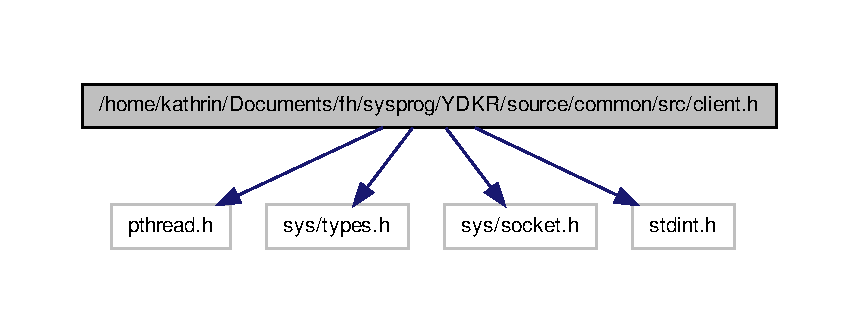
\includegraphics[width=400pt]{common_2src_2client_8h__incl}
\end{center}
\end{figure}
\subsection*{Data Structures}
\begin{DoxyCompactItemize}
\item 
struct \hyperlink{structclient__info}{client\_\-info}
\end{DoxyCompactItemize}
\subsection*{Defines}
\begin{DoxyCompactItemize}
\item 
\#define \hyperlink{common_2src_2client_8h_a4f600023423086559a0691f81d33da1b}{COMMON\_\-CLIENT\_\-H}
\end{DoxyCompactItemize}
\subsection*{Typedefs}
\begin{DoxyCompactItemize}
\item 
typedef struct \hyperlink{structclient__info}{client\_\-info} \hyperlink{common_2src_2client_8h_a0ff96238650bf51f4e5734af698b6454}{t\_\-client\_\-info}
\item 
typedef \hyperlink{structclient__info}{t\_\-client\_\-info} $\ast$ \hyperlink{common_2src_2client_8h_a3ac07717e32cd68b0ae357d638f1ac1e}{tp\_\-client\_\-info}
\end{DoxyCompactItemize}


\subsection{Define Documentation}
\hypertarget{common_2src_2client_8h_a4f600023423086559a0691f81d33da1b}{
\index{common/src/client.h@{common/src/client.h}!COMMON\_\-CLIENT\_\-H@{COMMON\_\-CLIENT\_\-H}}
\index{COMMON\_\-CLIENT\_\-H@{COMMON\_\-CLIENT\_\-H}!common/src/client.h@{common/src/client.h}}
\subsubsection[{COMMON\_\-CLIENT\_\-H}]{\setlength{\rightskip}{0pt plus 5cm}\#define COMMON\_\-CLIENT\_\-H}}
\label{common_2src_2client_8h_a4f600023423086559a0691f81d33da1b}


\subsection{Typedef Documentation}
\hypertarget{common_2src_2client_8h_a0ff96238650bf51f4e5734af698b6454}{
\index{common/src/client.h@{common/src/client.h}!t\_\-client\_\-info@{t\_\-client\_\-info}}
\index{t\_\-client\_\-info@{t\_\-client\_\-info}!common/src/client.h@{common/src/client.h}}
\subsubsection[{t\_\-client\_\-info}]{\setlength{\rightskip}{0pt plus 5cm}typedef struct {\bf client\_\-info} {\bf t\_\-client\_\-info}}}
\label{common_2src_2client_8h_a0ff96238650bf51f4e5734af698b6454}
\hypertarget{common_2src_2client_8h_a3ac07717e32cd68b0ae357d638f1ac1e}{
\index{common/src/client.h@{common/src/client.h}!tp\_\-client\_\-info@{tp\_\-client\_\-info}}
\index{tp\_\-client\_\-info@{tp\_\-client\_\-info}!common/src/client.h@{common/src/client.h}}
\subsubsection[{tp\_\-client\_\-info}]{\setlength{\rightskip}{0pt plus 5cm}typedef {\bf t\_\-client\_\-info}$\ast$ {\bf tp\_\-client\_\-info}}}
\label{common_2src_2client_8h_a3ac07717e32cd68b0ae357d638f1ac1e}

\hypertarget{fragewechsel_8c}{
\section{/home/kathrin/Documents/fh/sysprog/YDKR/source/client/src/fragewechsel.c File Reference}
\label{fragewechsel_8c}\index{/home/kathrin/Documents/fh/sysprog/YDKR/source/client/src/fragewechsel.c@{/home/kathrin/Documents/fh/sysprog/YDKR/source/client/src/fragewechsel.c}}
}
{\ttfamily \#include $<$stdio.h$>$}\par
{\ttfamily \#include $<$stdlib.h$>$}\par
{\ttfamily \#include $<$string.h$>$}\par
{\ttfamily \#include $<$sys/time.h$>$}\par
{\ttfamily \#include $<$sys/types.h$>$}\par
{\ttfamily \#include $<$unistd.h$>$}\par
{\ttfamily \#include $<$sys/socket.h$>$}\par
{\ttfamily \#include $<$errno.h$>$}\par
{\ttfamily \#include $<$netdb.h$>$}\par
{\ttfamily \#include $<$netinet/in.h$>$}\par
{\ttfamily \#include $<$arpa/inet.h$>$}\par
{\ttfamily \#include $<$getopt.h$>$}\par
{\ttfamily \#include \char`\"{}gui\_\-interface.h\char`\"{}}\par
{\ttfamily \#include \char`\"{}client.h\char`\"{}}\par
{\ttfamily \#include \char`\"{}listener.h\char`\"{}}\par
{\ttfamily \#include \char`\"{}fragewechsel.h\char`\"{}}\par
Include dependency graph for fragewechsel.c:
\nopagebreak
\begin{figure}[H]
\begin{center}
\leavevmode
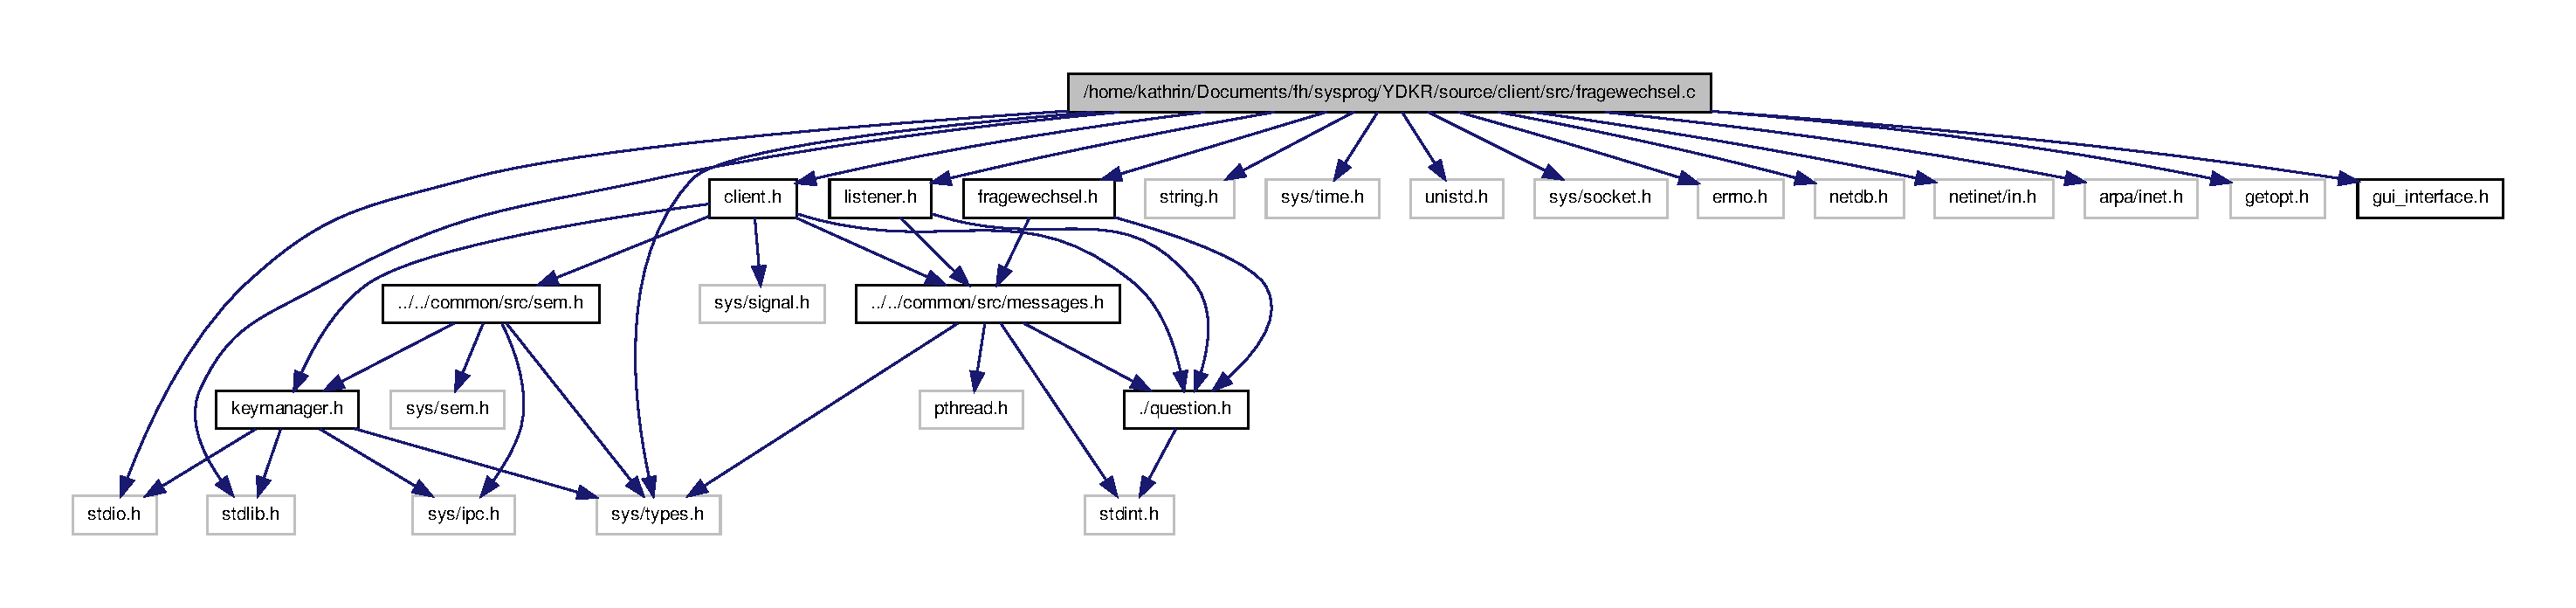
\includegraphics[width=400pt]{fragewechsel_8c__incl}
\end{center}
\end{figure}
\subsection*{Functions}
\begin{DoxyCompactItemize}
\item 
void $\ast$ \hyperlink{fragewechsel_8c_a94a96d85fb5e9d72948bfcc9efbc6f61}{fragen\_\-thread} (void $\ast$data)
\begin{DoxyCompactList}\small\item\em thread which calls send\_\-QR function if sempahore is free ================================================================= \item\end{DoxyCompactList}\end{DoxyCompactItemize}


\subsection{Detailed Description}
============================================================================

\begin{DoxyAuthor}{Author}
: Kathrin Holzmann 
\end{DoxyAuthor}
\begin{DoxyDate}{Date}
: Jun 20, 2011 ============================================================================ 
\end{DoxyDate}


\subsection{Function Documentation}
\hypertarget{fragewechsel_8c_a94a96d85fb5e9d72948bfcc9efbc6f61}{
\index{fragewechsel.c@{fragewechsel.c}!fragen\_\-thread@{fragen\_\-thread}}
\index{fragen\_\-thread@{fragen\_\-thread}!fragewechsel.c@{fragewechsel.c}}
\subsubsection[{fragen\_\-thread}]{\setlength{\rightskip}{0pt plus 5cm}void$\ast$ fragen\_\-thread (
\begin{DoxyParamCaption}
\item[{void $\ast$}]{data}
\end{DoxyParamCaption}
)}}
\label{fragewechsel_8c_a94a96d85fb5e9d72948bfcc9efbc6f61}


thread which calls send\_\-QR function if sempahore is free ================================================================= 

================================================================ 
\hypertarget{fragewechsel_8h}{
\section{/home/kathrin/Documents/fh/sysprog/YDKR/source/client/src/fragewechsel.h File Reference}
\label{fragewechsel_8h}\index{/home/kathrin/Documents/fh/sysprog/YDKR/source/client/src/fragewechsel.h@{/home/kathrin/Documents/fh/sysprog/YDKR/source/client/src/fragewechsel.h}}
}
{\ttfamily \#include \char`\"{}../../common/src/messages.h\char`\"{}}\par
{\ttfamily \#include \char`\"{}../../common/src/question.h\char`\"{}}\par
Include dependency graph for fragewechsel.h:
\nopagebreak
\begin{figure}[H]
\begin{center}
\leavevmode
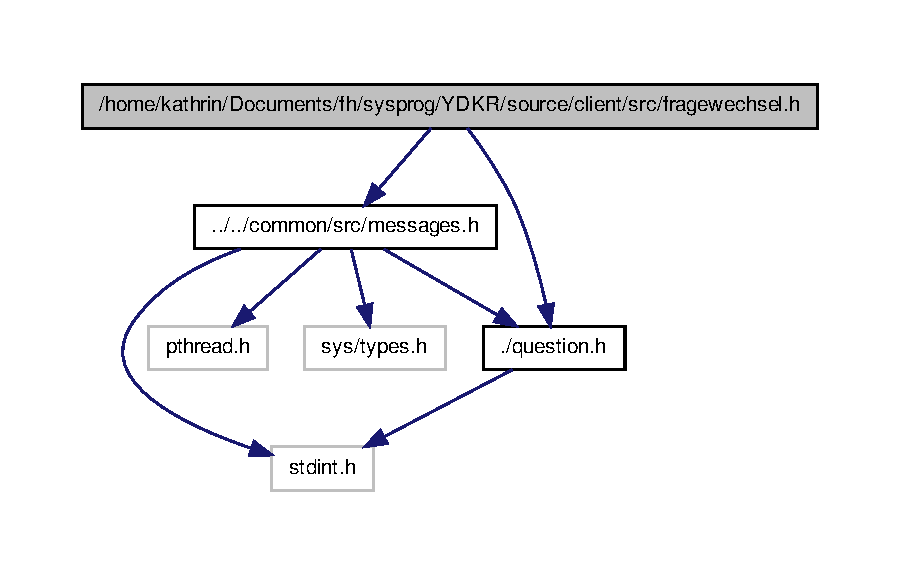
\includegraphics[width=400pt]{fragewechsel_8h__incl}
\end{center}
\end{figure}
This graph shows which files directly or indirectly include this file:
\nopagebreak
\begin{figure}[H]
\begin{center}
\leavevmode
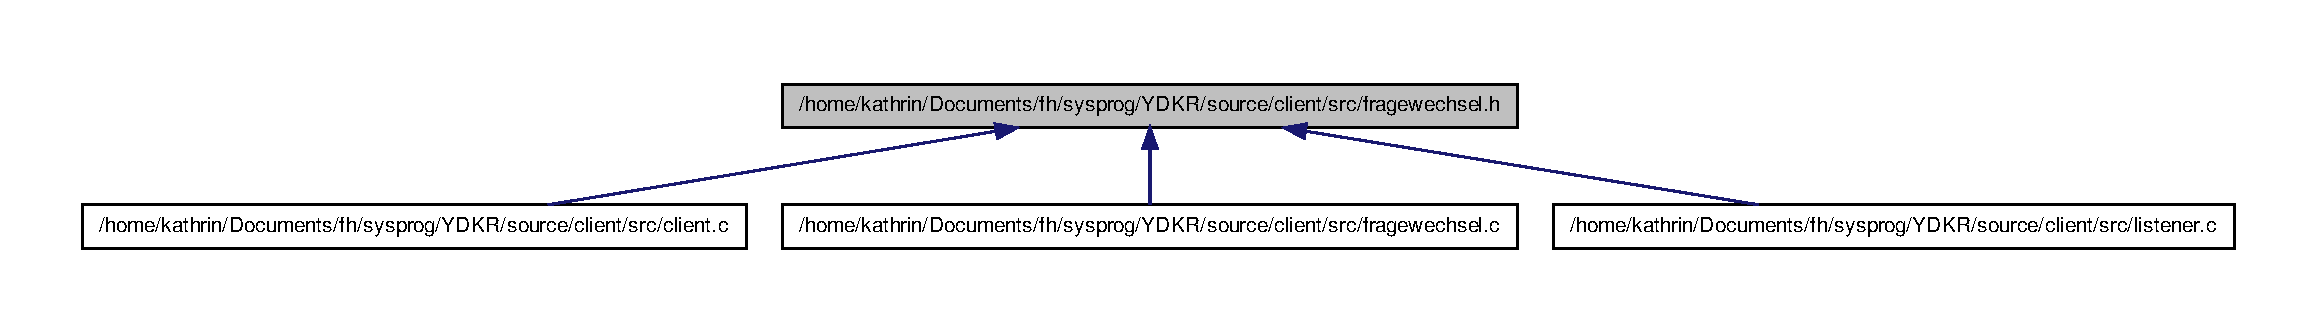
\includegraphics[width=400pt]{fragewechsel_8h__dep__incl}
\end{center}
\end{figure}
\subsection*{Functions}
\begin{DoxyCompactItemize}
\item 
void $\ast$ \hyperlink{fragewechsel_8h_a94a96d85fb5e9d72948bfcc9efbc6f61}{fragen\_\-thread} (void $\ast$data)
\begin{DoxyCompactList}\small\item\em thread which calls send\_\-QR function if sempahore is free ================================================================= \item\end{DoxyCompactList}\end{DoxyCompactItemize}


\subsection{Detailed Description}
============================================================================

\begin{DoxyAuthor}{Author}
: Kathrin Holzmann 
\end{DoxyAuthor}
\begin{DoxyDate}{Date}
: Jun 20, 2011 ============================================================================ 
\end{DoxyDate}


\subsection{Function Documentation}
\hypertarget{fragewechsel_8h_a94a96d85fb5e9d72948bfcc9efbc6f61}{
\index{fragewechsel.h@{fragewechsel.h}!fragen\_\-thread@{fragen\_\-thread}}
\index{fragen\_\-thread@{fragen\_\-thread}!fragewechsel.h@{fragewechsel.h}}
\subsubsection[{fragen\_\-thread}]{\setlength{\rightskip}{0pt plus 5cm}void$\ast$ fragen\_\-thread (
\begin{DoxyParamCaption}
\item[{void $\ast$}]{data}
\end{DoxyParamCaption}
)}}
\label{fragewechsel_8h_a94a96d85fb5e9d72948bfcc9efbc6f61}


thread which calls send\_\-QR function if sempahore is free ================================================================= 

================================================================ 
\hypertarget{gui_8h}{
\section{/home/kathrin/Documents/fh/sysprog/YDKR/source/client/src/gui.h File Reference}
\label{gui_8h}\index{/home/kathrin/Documents/fh/sysprog/YDKR/source/client/src/gui.h@{/home/kathrin/Documents/fh/sysprog/YDKR/source/client/src/gui.h}}
}
This graph shows which files directly or indirectly include this file:
\nopagebreak
\begin{figure}[H]
\begin{center}
\leavevmode
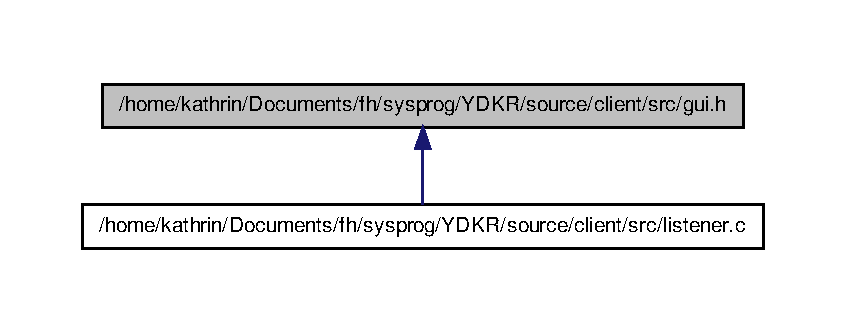
\includegraphics[width=400pt]{gui_8h__dep__incl}
\end{center}
\end{figure}

\hypertarget{gui__interface_8h}{
\section{/home/kathrin/Documents/fh/sysprog/YDKR/source/client/src/gui\_\-interface.h File Reference}
\label{gui__interface_8h}\index{/home/kathrin/Documents/fh/sysprog/YDKR/source/client/src/gui\_\-interface.h@{/home/kathrin/Documents/fh/sysprog/YDKR/source/client/src/gui\_\-interface.h}}
}
This graph shows which files directly or indirectly include this file:
\nopagebreak
\begin{figure}[H]
\begin{center}
\leavevmode
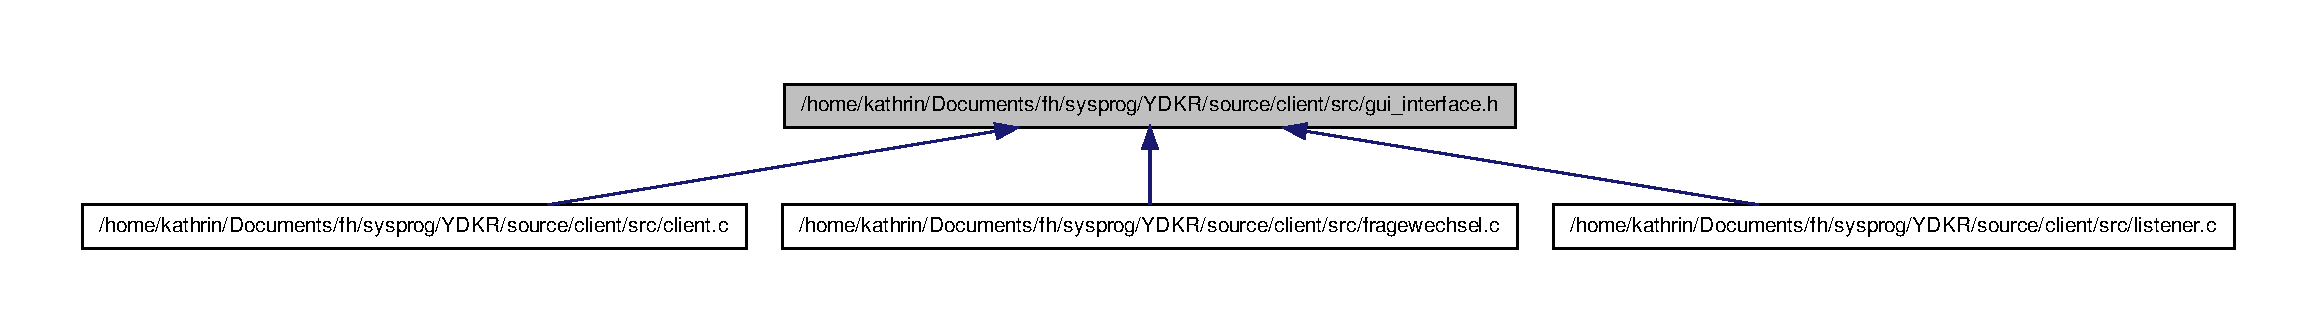
\includegraphics[width=400pt]{gui__interface_8h__dep__incl}
\end{center}
\end{figure}
\subsection*{Enumerations}
\begin{DoxyCompactItemize}
\item 
enum \{ \hyperlink{gui__interface_8h_a06fc87d81c62e9abb8790b6e5713c55bab4f1278da4bc7589a96802478485fd10}{GUI\_\-MAX\_\-USERS} =  6, 
\hyperlink{gui__interface_8h_a06fc87d81c62e9abb8790b6e5713c55ba7785d3316c59dbc69b19f63981942c89}{GUI\_\-NUM\_\-ANSWERS} =  4
 \}
\item 
enum \hyperlink{gui__interface_8h_a9002e872736dc09e98af8c2f1f6f5c56}{StatusIcon} \{ \hyperlink{gui__interface_8h_a9002e872736dc09e98af8c2f1f6f5c56a36bc4001254d4d0593a29b4a0ac65653}{STATUS\_\-ICON\_\-NONE} =  0, 
\hyperlink{gui__interface_8h_a9002e872736dc09e98af8c2f1f6f5c56ac2e1374f6a0e04d77f772684e875186b}{STATUS\_\-ICON\_\-CORRECT} =  1, 
\hyperlink{gui__interface_8h_a9002e872736dc09e98af8c2f1f6f5c56abea72006d82bedc88f9ab3fd0053b7a4}{STATUS\_\-ICON\_\-WRONG} =  2, 
\hyperlink{gui__interface_8h_a9002e872736dc09e98af8c2f1f6f5c56aff8a777fb949e5ac8e2bacc5cfb5314d}{STATUS\_\-ICON\_\-TIMEOUT} =  3
 \}
\begin{DoxyCompactList}\small\item\em Übergabewert für game\_\-setStatusIcon. \item\end{DoxyCompactList}\item 
enum \hyperlink{gui__interface_8h_ae5d479acbc4120e50d265a7a0fd50dee}{PreparationMode} \{ \hyperlink{gui__interface_8h_ae5d479acbc4120e50d265a7a0fd50deead33e46472ab55edf914ac6e17f49c416}{PREPARATION\_\-MODE\_\-BUSY} =  0, 
\hyperlink{gui__interface_8h_ae5d479acbc4120e50d265a7a0fd50deea4e49c1752049aed3217edcf80f85afe7}{PREPARATION\_\-MODE\_\-NORMAL} =  1, 
\hyperlink{gui__interface_8h_ae5d479acbc4120e50d265a7a0fd50deea88e87c22fd8676bfde95bb1cca5a4966}{PREPARATION\_\-MODE\_\-PRIVILEGED} =  2
 \}
\begin{DoxyCompactList}\small\item\em Übergabewert für preparation\_\-setMode. \item\end{DoxyCompactList}\end{DoxyCompactItemize}
\subsection*{Functions}
\begin{DoxyCompactItemize}
\item 
void \hyperlink{gui__interface_8h_a819bbcd1bc0fea1744a07658b92a4e12}{guiInit} (int $\ast$argc, char $\ast$$\ast$$\ast$argv)
\item 
void \hyperlink{gui__interface_8h_acfc60a28e55e1d7d5da60352b53044c7}{guiMain} (void)
\item 
void \hyperlink{gui__interface_8h_a2ec7878b1f11f1f134f79a07868d364a}{guiQuit} (void)
\item 
void \hyperlink{gui__interface_8h_a8ce970b7037206ed1ee356509e14b8a4}{guiDestroy} (void)
\item 
void \hyperlink{gui__interface_8h_a0a89a8fadecb0e31637d37a9d6deef1a}{guiShowErrorDialog} (const char $\ast$message, int quitOnClose)
\item 
void \hyperlink{gui__interface_8h_a066ee7949821ca5af3f4f2efde09a523}{guiShowMessageDialog} (const char $\ast$message, int quitOnClose)
\item 
void \hyperlink{gui__interface_8h_abb290af51dc45dcda93559994642f17a}{preparation\_\-setMode} (\hyperlink{gui__interface_8h_ae5d479acbc4120e50d265a7a0fd50dee}{PreparationMode} mode)
\item 
void \hyperlink{gui__interface_8h_a27762bb527640d590f562d914e6606c2}{preparation\_\-showWindow} (void)
\item 
void \hyperlink{gui__interface_8h_a334ee774572ceb7914a5857a24ab41b4}{preparation\_\-addCatalog} (const char $\ast$name)
\item 
int \hyperlink{gui__interface_8h_aece8101859ac86c33b7402fe26d3ae0d}{preparation\_\-selectCatalog} (const char $\ast$name)
\item 
void \hyperlink{gui__interface_8h_a218be68e749cd6cc4edfc0203754966c}{preparation\_\-addPlayer} (const char $\ast$name)
\item 
int \hyperlink{gui__interface_8h_a02f99539d4e3a7047621fc02b5ace4f2}{preparation\_\-removePlayer} (const char $\ast$name)
\item 
void \hyperlink{gui__interface_8h_ab49f6c6c7761e88c3844e03ffe347d0b}{preparation\_\-clearPlayers} (void)
\item 
void \hyperlink{gui__interface_8h_a36e5280b4ddf98dbdbdf1910bb965366}{preparation\_\-hideWindow} (void)
\item 
void \hyperlink{gui__interface_8h_aa07683aaf6fc9d5d4edd9a121451252f}{preparation\_\-reset} (void)
\item 
void \hyperlink{gui__interface_8h_ae1668ab012c3cdaddb0eb4f3f3f65bf4}{preparation\_\-onCatalogChanged} (const char $\ast$newSelection)
\item 
void \hyperlink{gui__interface_8h_a3fa54fc6ad4c3c005c34d965f485acc1}{preparation\_\-onStartClicked} (const char $\ast$currentSelection)
\item 
void \hyperlink{gui__interface_8h_aa0b6239c0fa80055895d9668c3cb8674}{preparation\_\-onWindowClosed} (void)
\item 
void \hyperlink{gui__interface_8h_a92a23d536ff75bbfa86bcd9e5a695fe9}{game\_\-showWindow} (void)
\item 
void \hyperlink{gui__interface_8h_ab56ef3132244269c5378371638b3064b}{game\_\-setStatusText} (const char $\ast$text)
\item 
void \hyperlink{gui__interface_8h_a55f8afa06033b467196ccd5a46225da3}{game\_\-setStatusIcon} (\hyperlink{gui__interface_8h_a9002e872736dc09e98af8c2f1f6f5c56}{StatusIcon} icon)
\item 
void \hyperlink{gui__interface_8h_a012d522d531fb1432569eaaf43e3d6ee}{game\_\-setQuestion} (const char $\ast$text)
\item 
void \hyperlink{gui__interface_8h_ad01c163ae271d8e3578f308f0922b8ff}{game\_\-setAnswer} (int index, const char $\ast$text)
\item 
void \hyperlink{gui__interface_8h_a3864747f4aad5d38f65d6ddf8ced5837}{game\_\-markAnswerCorrect} (int index)
\item 
void \hyperlink{gui__interface_8h_ac780657bd254c88b19bed16c9d44c702}{game\_\-markAnswerWrong} (int index)
\item 
void \hyperlink{gui__interface_8h_a08c12836896a6b4625f5bd209b3ccf2f}{game\_\-unmarkAnswers} (void)
\item 
void \hyperlink{gui__interface_8h_a58a363f236f29f8dc329bf276a0286e6}{game\_\-setAnswerButtonsEnabled} (int enable)
\item 
void \hyperlink{gui__interface_8h_af85faec39899017aefe4d46c2a5ad838}{game\_\-setPlayerName} (int position, const char $\ast$name)
\item 
void \hyperlink{gui__interface_8h_a3388d28c32ad891207cc22f245821e68}{game\_\-setPlayerScore} (int position, unsigned long score)
\item 
void \hyperlink{gui__interface_8h_a4eaf3c079eb53afb1d286f76b6d383a1}{game\_\-highlightPlayer} (int position)
\item 
void \hyperlink{gui__interface_8h_a409bf5d1890aceb9faa1129511b6fca4}{game\_\-hideWindow} (void)
\item 
void \hyperlink{gui__interface_8h_a05cddc86cdca6cac72dddefeaf3c142e}{game\_\-reset} (void)
\item 
void \hyperlink{gui__interface_8h_a497a03837ef1b64798d50914c1caa06f}{game\_\-onAnswerClicked} (int index)
\item 
void \hyperlink{gui__interface_8h_aac4987aa3c13f02fcaca620822dabfd1}{game\_\-onWindowClosed} (void)
\end{DoxyCompactItemize}


\subsection{Enumeration Type Documentation}
\hypertarget{gui__interface_8h_a06fc87d81c62e9abb8790b6e5713c55b}{
\subsubsection[{"@0}]{\setlength{\rightskip}{0pt plus 5cm}anonymous enum}}
\label{gui__interface_8h_a06fc87d81c62e9abb8790b6e5713c55b}
\begin{Desc}
\item[Enumerator: ]\par
\begin{description}
\index{GUI\_\-MAX\_\-USERS@{GUI\_\-MAX\_\-USERS}!gui\_\-interface.h@{gui\_\-interface.h}}\index{gui\_\-interface.h@{gui\_\-interface.h}!GUI\_\-MAX\_\-USERS@{GUI\_\-MAX\_\-USERS}}\item[{\em 
\hypertarget{gui__interface_8h_a06fc87d81c62e9abb8790b6e5713c55bab4f1278da4bc7589a96802478485fd10}{
GUI\_\-MAX\_\-USERS}
\label{gui__interface_8h_a06fc87d81c62e9abb8790b6e5713c55bab4f1278da4bc7589a96802478485fd10}
}]maximal 6 User \index{GUI\_\-NUM\_\-ANSWERS@{GUI\_\-NUM\_\-ANSWERS}!gui\_\-interface.h@{gui\_\-interface.h}}\index{gui\_\-interface.h@{gui\_\-interface.h}!GUI\_\-NUM\_\-ANSWERS@{GUI\_\-NUM\_\-ANSWERS}}\item[{\em 
\hypertarget{gui__interface_8h_a06fc87d81c62e9abb8790b6e5713c55ba7785d3316c59dbc69b19f63981942c89}{
GUI\_\-NUM\_\-ANSWERS}
\label{gui__interface_8h_a06fc87d81c62e9abb8790b6e5713c55ba7785d3316c59dbc69b19f63981942c89}
}]pro Frage 4 Antwortmöglichkeiten \end{description}
\end{Desc}

\hypertarget{gui__interface_8h_ae5d479acbc4120e50d265a7a0fd50dee}{
\index{gui\_\-interface.h@{gui\_\-interface.h}!PreparationMode@{PreparationMode}}
\index{PreparationMode@{PreparationMode}!gui_interface.h@{gui\_\-interface.h}}
\subsubsection[{PreparationMode}]{\setlength{\rightskip}{0pt plus 5cm}enum {\bf PreparationMode}}}
\label{gui__interface_8h_ae5d479acbc4120e50d265a7a0fd50dee}


Übergabewert für preparation\_\-setMode. 

Spezifiziert den Modus, in dem sich das Vorbereitungsfenster befindet. \begin{Desc}
\item[Enumerator: ]\par
\begin{description}
\index{PREPARATION\_\-MODE\_\-BUSY@{PREPARATION\_\-MODE\_\-BUSY}!gui\_\-interface.h@{gui\_\-interface.h}}\index{gui\_\-interface.h@{gui\_\-interface.h}!PREPARATION\_\-MODE\_\-BUSY@{PREPARATION\_\-MODE\_\-BUSY}}\item[{\em 
\hypertarget{gui__interface_8h_ae5d479acbc4120e50d265a7a0fd50deead33e46472ab55edf914ac6e17f49c416}{
PREPARATION\_\-MODE\_\-BUSY}
\label{gui__interface_8h_ae5d479acbc4120e50d265a7a0fd50deead33e46472ab55edf914ac6e17f49c416}
}]Momentan beschäftigt, es werden keine Eingaben zugelassen \index{PREPARATION\_\-MODE\_\-NORMAL@{PREPARATION\_\-MODE\_\-NORMAL}!gui\_\-interface.h@{gui\_\-interface.h}}\index{gui\_\-interface.h@{gui\_\-interface.h}!PREPARATION\_\-MODE\_\-NORMAL@{PREPARATION\_\-MODE\_\-NORMAL}}\item[{\em 
\hypertarget{gui__interface_8h_ae5d479acbc4120e50d265a7a0fd50deea4e49c1752049aed3217edcf80f85afe7}{
PREPARATION\_\-MODE\_\-NORMAL}
\label{gui__interface_8h_ae5d479acbc4120e50d265a7a0fd50deea4e49c1752049aed3217edcf80f85afe7}
}]Normaler Modus, Katalogauswahl und Start durch User nicht möglich \index{PREPARATION\_\-MODE\_\-PRIVILEGED@{PREPARATION\_\-MODE\_\-PRIVILEGED}!gui\_\-interface.h@{gui\_\-interface.h}}\index{gui\_\-interface.h@{gui\_\-interface.h}!PREPARATION\_\-MODE\_\-PRIVILEGED@{PREPARATION\_\-MODE\_\-PRIVILEGED}}\item[{\em 
\hypertarget{gui__interface_8h_ae5d479acbc4120e50d265a7a0fd50deea88e87c22fd8676bfde95bb1cca5a4966}{
PREPARATION\_\-MODE\_\-PRIVILEGED}
\label{gui__interface_8h_ae5d479acbc4120e50d265a7a0fd50deea88e87c22fd8676bfde95bb1cca5a4966}
}]Modus für den Spielleiter, Katalogauswahl und Start möglich \end{description}
\end{Desc}

\hypertarget{gui__interface_8h_a9002e872736dc09e98af8c2f1f6f5c56}{
\index{gui\_\-interface.h@{gui\_\-interface.h}!StatusIcon@{StatusIcon}}
\index{StatusIcon@{StatusIcon}!gui_interface.h@{gui\_\-interface.h}}
\subsubsection[{StatusIcon}]{\setlength{\rightskip}{0pt plus 5cm}enum {\bf StatusIcon}}}
\label{gui__interface_8h_a9002e872736dc09e98af8c2f1f6f5c56}


Übergabewert für game\_\-setStatusIcon. 

Spezifiziert das in der Statuszeile des Spielfenster anzuzeigende Icon. \begin{Desc}
\item[Enumerator: ]\par
\begin{description}
\index{STATUS\_\-ICON\_\-NONE@{STATUS\_\-ICON\_\-NONE}!gui\_\-interface.h@{gui\_\-interface.h}}\index{gui\_\-interface.h@{gui\_\-interface.h}!STATUS\_\-ICON\_\-NONE@{STATUS\_\-ICON\_\-NONE}}\item[{\em 
\hypertarget{gui__interface_8h_a9002e872736dc09e98af8c2f1f6f5c56a36bc4001254d4d0593a29b4a0ac65653}{
STATUS\_\-ICON\_\-NONE}
\label{gui__interface_8h_a9002e872736dc09e98af8c2f1f6f5c56a36bc4001254d4d0593a29b4a0ac65653}
}]Kein Statusicon anzeigen \index{STATUS\_\-ICON\_\-CORRECT@{STATUS\_\-ICON\_\-CORRECT}!gui\_\-interface.h@{gui\_\-interface.h}}\index{gui\_\-interface.h@{gui\_\-interface.h}!STATUS\_\-ICON\_\-CORRECT@{STATUS\_\-ICON\_\-CORRECT}}\item[{\em 
\hypertarget{gui__interface_8h_a9002e872736dc09e98af8c2f1f6f5c56ac2e1374f6a0e04d77f772684e875186b}{
STATUS\_\-ICON\_\-CORRECT}
\label{gui__interface_8h_a9002e872736dc09e98af8c2f1f6f5c56ac2e1374f6a0e04d77f772684e875186b}
}]Icon für richtige Antwort anzeigen \index{STATUS\_\-ICON\_\-WRONG@{STATUS\_\-ICON\_\-WRONG}!gui\_\-interface.h@{gui\_\-interface.h}}\index{gui\_\-interface.h@{gui\_\-interface.h}!STATUS\_\-ICON\_\-WRONG@{STATUS\_\-ICON\_\-WRONG}}\item[{\em 
\hypertarget{gui__interface_8h_a9002e872736dc09e98af8c2f1f6f5c56abea72006d82bedc88f9ab3fd0053b7a4}{
STATUS\_\-ICON\_\-WRONG}
\label{gui__interface_8h_a9002e872736dc09e98af8c2f1f6f5c56abea72006d82bedc88f9ab3fd0053b7a4}
}]Icon für falsche Antwort anzeigen \index{STATUS\_\-ICON\_\-TIMEOUT@{STATUS\_\-ICON\_\-TIMEOUT}!gui\_\-interface.h@{gui\_\-interface.h}}\index{gui\_\-interface.h@{gui\_\-interface.h}!STATUS\_\-ICON\_\-TIMEOUT@{STATUS\_\-ICON\_\-TIMEOUT}}\item[{\em 
\hypertarget{gui__interface_8h_a9002e872736dc09e98af8c2f1f6f5c56aff8a777fb949e5ac8e2bacc5cfb5314d}{
STATUS\_\-ICON\_\-TIMEOUT}
\label{gui__interface_8h_a9002e872736dc09e98af8c2f1f6f5c56aff8a777fb949e5ac8e2bacc5cfb5314d}
}]Icon für \char`\"{}Zeit abgelaufen\char`\"{} anzeigen \end{description}
\end{Desc}



\subsection{Function Documentation}
\hypertarget{gui__interface_8h_a409bf5d1890aceb9faa1129511b6fca4}{
\index{gui\_\-interface.h@{gui\_\-interface.h}!game\_\-hideWindow@{game\_\-hideWindow}}
\index{game\_\-hideWindow@{game\_\-hideWindow}!gui_interface.h@{gui\_\-interface.h}}
\subsubsection[{game\_\-hideWindow}]{\setlength{\rightskip}{0pt plus 5cm}void game\_\-hideWindow (
\begin{DoxyParamCaption}
\item[{void}]{}
\end{DoxyParamCaption}
)}}
\label{gui__interface_8h_a409bf5d1890aceb9faa1129511b6fca4}
\hypertarget{gui__interface_8h_a4eaf3c079eb53afb1d286f76b6d383a1}{
\index{gui\_\-interface.h@{gui\_\-interface.h}!game\_\-highlightPlayer@{game\_\-highlightPlayer}}
\index{game\_\-highlightPlayer@{game\_\-highlightPlayer}!gui_interface.h@{gui\_\-interface.h}}
\subsubsection[{game\_\-highlightPlayer}]{\setlength{\rightskip}{0pt plus 5cm}void game\_\-highlightPlayer (
\begin{DoxyParamCaption}
\item[{int}]{position}
\end{DoxyParamCaption}
)}}
\label{gui__interface_8h_a4eaf3c079eb53afb1d286f76b6d383a1}
\hypertarget{gui__interface_8h_a3864747f4aad5d38f65d6ddf8ced5837}{
\index{gui\_\-interface.h@{gui\_\-interface.h}!game\_\-markAnswerCorrect@{game\_\-markAnswerCorrect}}
\index{game\_\-markAnswerCorrect@{game\_\-markAnswerCorrect}!gui_interface.h@{gui\_\-interface.h}}
\subsubsection[{game\_\-markAnswerCorrect}]{\setlength{\rightskip}{0pt plus 5cm}void game\_\-markAnswerCorrect (
\begin{DoxyParamCaption}
\item[{int}]{index}
\end{DoxyParamCaption}
)}}
\label{gui__interface_8h_a3864747f4aad5d38f65d6ddf8ced5837}
\hypertarget{gui__interface_8h_ac780657bd254c88b19bed16c9d44c702}{
\index{gui\_\-interface.h@{gui\_\-interface.h}!game\_\-markAnswerWrong@{game\_\-markAnswerWrong}}
\index{game\_\-markAnswerWrong@{game\_\-markAnswerWrong}!gui_interface.h@{gui\_\-interface.h}}
\subsubsection[{game\_\-markAnswerWrong}]{\setlength{\rightskip}{0pt plus 5cm}void game\_\-markAnswerWrong (
\begin{DoxyParamCaption}
\item[{int}]{index}
\end{DoxyParamCaption}
)}}
\label{gui__interface_8h_ac780657bd254c88b19bed16c9d44c702}
\hypertarget{gui__interface_8h_a497a03837ef1b64798d50914c1caa06f}{
\index{gui\_\-interface.h@{gui\_\-interface.h}!game\_\-onAnswerClicked@{game\_\-onAnswerClicked}}
\index{game\_\-onAnswerClicked@{game\_\-onAnswerClicked}!gui_interface.h@{gui\_\-interface.h}}
\subsubsection[{game\_\-onAnswerClicked}]{\setlength{\rightskip}{0pt plus 5cm}void game\_\-onAnswerClicked (
\begin{DoxyParamCaption}
\item[{int}]{index}
\end{DoxyParamCaption}
)}}
\label{gui__interface_8h_a497a03837ef1b64798d50914c1caa06f}
\hypertarget{gui__interface_8h_aac4987aa3c13f02fcaca620822dabfd1}{
\index{gui\_\-interface.h@{gui\_\-interface.h}!game\_\-onWindowClosed@{game\_\-onWindowClosed}}
\index{game\_\-onWindowClosed@{game\_\-onWindowClosed}!gui_interface.h@{gui\_\-interface.h}}
\subsubsection[{game\_\-onWindowClosed}]{\setlength{\rightskip}{0pt plus 5cm}void game\_\-onWindowClosed (
\begin{DoxyParamCaption}
\item[{void}]{}
\end{DoxyParamCaption}
)}}
\label{gui__interface_8h_aac4987aa3c13f02fcaca620822dabfd1}
\hypertarget{gui__interface_8h_a05cddc86cdca6cac72dddefeaf3c142e}{
\index{gui\_\-interface.h@{gui\_\-interface.h}!game\_\-reset@{game\_\-reset}}
\index{game\_\-reset@{game\_\-reset}!gui_interface.h@{gui\_\-interface.h}}
\subsubsection[{game\_\-reset}]{\setlength{\rightskip}{0pt plus 5cm}void game\_\-reset (
\begin{DoxyParamCaption}
\item[{void}]{}
\end{DoxyParamCaption}
)}}
\label{gui__interface_8h_a05cddc86cdca6cac72dddefeaf3c142e}
\hypertarget{gui__interface_8h_ad01c163ae271d8e3578f308f0922b8ff}{
\index{gui\_\-interface.h@{gui\_\-interface.h}!game\_\-setAnswer@{game\_\-setAnswer}}
\index{game\_\-setAnswer@{game\_\-setAnswer}!gui_interface.h@{gui\_\-interface.h}}
\subsubsection[{game\_\-setAnswer}]{\setlength{\rightskip}{0pt plus 5cm}void game\_\-setAnswer (
\begin{DoxyParamCaption}
\item[{int}]{index, }
\item[{const char $\ast$}]{text}
\end{DoxyParamCaption}
)}}
\label{gui__interface_8h_ad01c163ae271d8e3578f308f0922b8ff}
\hypertarget{gui__interface_8h_a58a363f236f29f8dc329bf276a0286e6}{
\index{gui\_\-interface.h@{gui\_\-interface.h}!game\_\-setAnswerButtonsEnabled@{game\_\-setAnswerButtonsEnabled}}
\index{game\_\-setAnswerButtonsEnabled@{game\_\-setAnswerButtonsEnabled}!gui_interface.h@{gui\_\-interface.h}}
\subsubsection[{game\_\-setAnswerButtonsEnabled}]{\setlength{\rightskip}{0pt plus 5cm}void game\_\-setAnswerButtonsEnabled (
\begin{DoxyParamCaption}
\item[{int}]{enable}
\end{DoxyParamCaption}
)}}
\label{gui__interface_8h_a58a363f236f29f8dc329bf276a0286e6}
\hypertarget{gui__interface_8h_af85faec39899017aefe4d46c2a5ad838}{
\index{gui\_\-interface.h@{gui\_\-interface.h}!game\_\-setPlayerName@{game\_\-setPlayerName}}
\index{game\_\-setPlayerName@{game\_\-setPlayerName}!gui_interface.h@{gui\_\-interface.h}}
\subsubsection[{game\_\-setPlayerName}]{\setlength{\rightskip}{0pt plus 5cm}void game\_\-setPlayerName (
\begin{DoxyParamCaption}
\item[{int}]{position, }
\item[{const char $\ast$}]{name}
\end{DoxyParamCaption}
)}}
\label{gui__interface_8h_af85faec39899017aefe4d46c2a5ad838}
\hypertarget{gui__interface_8h_a3388d28c32ad891207cc22f245821e68}{
\index{gui\_\-interface.h@{gui\_\-interface.h}!game\_\-setPlayerScore@{game\_\-setPlayerScore}}
\index{game\_\-setPlayerScore@{game\_\-setPlayerScore}!gui_interface.h@{gui\_\-interface.h}}
\subsubsection[{game\_\-setPlayerScore}]{\setlength{\rightskip}{0pt plus 5cm}void game\_\-setPlayerScore (
\begin{DoxyParamCaption}
\item[{int}]{position, }
\item[{unsigned long}]{score}
\end{DoxyParamCaption}
)}}
\label{gui__interface_8h_a3388d28c32ad891207cc22f245821e68}
\hypertarget{gui__interface_8h_a012d522d531fb1432569eaaf43e3d6ee}{
\index{gui\_\-interface.h@{gui\_\-interface.h}!game\_\-setQuestion@{game\_\-setQuestion}}
\index{game\_\-setQuestion@{game\_\-setQuestion}!gui_interface.h@{gui\_\-interface.h}}
\subsubsection[{game\_\-setQuestion}]{\setlength{\rightskip}{0pt plus 5cm}void game\_\-setQuestion (
\begin{DoxyParamCaption}
\item[{const char $\ast$}]{text}
\end{DoxyParamCaption}
)}}
\label{gui__interface_8h_a012d522d531fb1432569eaaf43e3d6ee}
\hypertarget{gui__interface_8h_a55f8afa06033b467196ccd5a46225da3}{
\index{gui\_\-interface.h@{gui\_\-interface.h}!game\_\-setStatusIcon@{game\_\-setStatusIcon}}
\index{game\_\-setStatusIcon@{game\_\-setStatusIcon}!gui_interface.h@{gui\_\-interface.h}}
\subsubsection[{game\_\-setStatusIcon}]{\setlength{\rightskip}{0pt plus 5cm}void game\_\-setStatusIcon (
\begin{DoxyParamCaption}
\item[{{\bf StatusIcon}}]{icon}
\end{DoxyParamCaption}
)}}
\label{gui__interface_8h_a55f8afa06033b467196ccd5a46225da3}
\hypertarget{gui__interface_8h_ab56ef3132244269c5378371638b3064b}{
\index{gui\_\-interface.h@{gui\_\-interface.h}!game\_\-setStatusText@{game\_\-setStatusText}}
\index{game\_\-setStatusText@{game\_\-setStatusText}!gui_interface.h@{gui\_\-interface.h}}
\subsubsection[{game\_\-setStatusText}]{\setlength{\rightskip}{0pt plus 5cm}void game\_\-setStatusText (
\begin{DoxyParamCaption}
\item[{const char $\ast$}]{text}
\end{DoxyParamCaption}
)}}
\label{gui__interface_8h_ab56ef3132244269c5378371638b3064b}
\hypertarget{gui__interface_8h_a92a23d536ff75bbfa86bcd9e5a695fe9}{
\index{gui\_\-interface.h@{gui\_\-interface.h}!game\_\-showWindow@{game\_\-showWindow}}
\index{game\_\-showWindow@{game\_\-showWindow}!gui_interface.h@{gui\_\-interface.h}}
\subsubsection[{game\_\-showWindow}]{\setlength{\rightskip}{0pt plus 5cm}void game\_\-showWindow (
\begin{DoxyParamCaption}
\item[{void}]{}
\end{DoxyParamCaption}
)}}
\label{gui__interface_8h_a92a23d536ff75bbfa86bcd9e5a695fe9}
\hypertarget{gui__interface_8h_a08c12836896a6b4625f5bd209b3ccf2f}{
\index{gui\_\-interface.h@{gui\_\-interface.h}!game\_\-unmarkAnswers@{game\_\-unmarkAnswers}}
\index{game\_\-unmarkAnswers@{game\_\-unmarkAnswers}!gui_interface.h@{gui\_\-interface.h}}
\subsubsection[{game\_\-unmarkAnswers}]{\setlength{\rightskip}{0pt plus 5cm}void game\_\-unmarkAnswers (
\begin{DoxyParamCaption}
\item[{void}]{}
\end{DoxyParamCaption}
)}}
\label{gui__interface_8h_a08c12836896a6b4625f5bd209b3ccf2f}
\hypertarget{gui__interface_8h_a8ce970b7037206ed1ee356509e14b8a4}{
\index{gui\_\-interface.h@{gui\_\-interface.h}!guiDestroy@{guiDestroy}}
\index{guiDestroy@{guiDestroy}!gui_interface.h@{gui\_\-interface.h}}
\subsubsection[{guiDestroy}]{\setlength{\rightskip}{0pt plus 5cm}void guiDestroy (
\begin{DoxyParamCaption}
\item[{void}]{}
\end{DoxyParamCaption}
)}}
\label{gui__interface_8h_a8ce970b7037206ed1ee356509e14b8a4}
\hypertarget{gui__interface_8h_a819bbcd1bc0fea1744a07658b92a4e12}{
\index{gui\_\-interface.h@{gui\_\-interface.h}!guiInit@{guiInit}}
\index{guiInit@{guiInit}!gui_interface.h@{gui\_\-interface.h}}
\subsubsection[{guiInit}]{\setlength{\rightskip}{0pt plus 5cm}void guiInit (
\begin{DoxyParamCaption}
\item[{int $\ast$}]{argc, }
\item[{char $\ast$$\ast$$\ast$}]{argv}
\end{DoxyParamCaption}
)}}
\label{gui__interface_8h_a819bbcd1bc0fea1744a07658b92a4e12}
\hypertarget{gui__interface_8h_acfc60a28e55e1d7d5da60352b53044c7}{
\index{gui\_\-interface.h@{gui\_\-interface.h}!guiMain@{guiMain}}
\index{guiMain@{guiMain}!gui_interface.h@{gui\_\-interface.h}}
\subsubsection[{guiMain}]{\setlength{\rightskip}{0pt plus 5cm}void guiMain (
\begin{DoxyParamCaption}
\item[{void}]{}
\end{DoxyParamCaption}
)}}
\label{gui__interface_8h_acfc60a28e55e1d7d5da60352b53044c7}
\hypertarget{gui__interface_8h_a2ec7878b1f11f1f134f79a07868d364a}{
\index{gui\_\-interface.h@{gui\_\-interface.h}!guiQuit@{guiQuit}}
\index{guiQuit@{guiQuit}!gui_interface.h@{gui\_\-interface.h}}
\subsubsection[{guiQuit}]{\setlength{\rightskip}{0pt plus 5cm}void guiQuit (
\begin{DoxyParamCaption}
\item[{void}]{}
\end{DoxyParamCaption}
)}}
\label{gui__interface_8h_a2ec7878b1f11f1f134f79a07868d364a}
\hypertarget{gui__interface_8h_a0a89a8fadecb0e31637d37a9d6deef1a}{
\index{gui\_\-interface.h@{gui\_\-interface.h}!guiShowErrorDialog@{guiShowErrorDialog}}
\index{guiShowErrorDialog@{guiShowErrorDialog}!gui_interface.h@{gui\_\-interface.h}}
\subsubsection[{guiShowErrorDialog}]{\setlength{\rightskip}{0pt plus 5cm}void guiShowErrorDialog (
\begin{DoxyParamCaption}
\item[{const char $\ast$}]{message, }
\item[{int}]{quitOnClose}
\end{DoxyParamCaption}
)}}
\label{gui__interface_8h_a0a89a8fadecb0e31637d37a9d6deef1a}
\hypertarget{gui__interface_8h_a066ee7949821ca5af3f4f2efde09a523}{
\index{gui\_\-interface.h@{gui\_\-interface.h}!guiShowMessageDialog@{guiShowMessageDialog}}
\index{guiShowMessageDialog@{guiShowMessageDialog}!gui_interface.h@{gui\_\-interface.h}}
\subsubsection[{guiShowMessageDialog}]{\setlength{\rightskip}{0pt plus 5cm}void guiShowMessageDialog (
\begin{DoxyParamCaption}
\item[{const char $\ast$}]{message, }
\item[{int}]{quitOnClose}
\end{DoxyParamCaption}
)}}
\label{gui__interface_8h_a066ee7949821ca5af3f4f2efde09a523}
\hypertarget{gui__interface_8h_a334ee774572ceb7914a5857a24ab41b4}{
\index{gui\_\-interface.h@{gui\_\-interface.h}!preparation\_\-addCatalog@{preparation\_\-addCatalog}}
\index{preparation\_\-addCatalog@{preparation\_\-addCatalog}!gui_interface.h@{gui\_\-interface.h}}
\subsubsection[{preparation\_\-addCatalog}]{\setlength{\rightskip}{0pt plus 5cm}void preparation\_\-addCatalog (
\begin{DoxyParamCaption}
\item[{const char $\ast$}]{name}
\end{DoxyParamCaption}
)}}
\label{gui__interface_8h_a334ee774572ceb7914a5857a24ab41b4}
\hypertarget{gui__interface_8h_a218be68e749cd6cc4edfc0203754966c}{
\index{gui\_\-interface.h@{gui\_\-interface.h}!preparation\_\-addPlayer@{preparation\_\-addPlayer}}
\index{preparation\_\-addPlayer@{preparation\_\-addPlayer}!gui_interface.h@{gui\_\-interface.h}}
\subsubsection[{preparation\_\-addPlayer}]{\setlength{\rightskip}{0pt plus 5cm}void preparation\_\-addPlayer (
\begin{DoxyParamCaption}
\item[{const char $\ast$}]{name}
\end{DoxyParamCaption}
)}}
\label{gui__interface_8h_a218be68e749cd6cc4edfc0203754966c}
\hypertarget{gui__interface_8h_ab49f6c6c7761e88c3844e03ffe347d0b}{
\index{gui\_\-interface.h@{gui\_\-interface.h}!preparation\_\-clearPlayers@{preparation\_\-clearPlayers}}
\index{preparation\_\-clearPlayers@{preparation\_\-clearPlayers}!gui_interface.h@{gui\_\-interface.h}}
\subsubsection[{preparation\_\-clearPlayers}]{\setlength{\rightskip}{0pt plus 5cm}void preparation\_\-clearPlayers (
\begin{DoxyParamCaption}
\item[{void}]{}
\end{DoxyParamCaption}
)}}
\label{gui__interface_8h_ab49f6c6c7761e88c3844e03ffe347d0b}
\hypertarget{gui__interface_8h_a36e5280b4ddf98dbdbdf1910bb965366}{
\index{gui\_\-interface.h@{gui\_\-interface.h}!preparation\_\-hideWindow@{preparation\_\-hideWindow}}
\index{preparation\_\-hideWindow@{preparation\_\-hideWindow}!gui_interface.h@{gui\_\-interface.h}}
\subsubsection[{preparation\_\-hideWindow}]{\setlength{\rightskip}{0pt plus 5cm}void preparation\_\-hideWindow (
\begin{DoxyParamCaption}
\item[{void}]{}
\end{DoxyParamCaption}
)}}
\label{gui__interface_8h_a36e5280b4ddf98dbdbdf1910bb965366}
\hypertarget{gui__interface_8h_ae1668ab012c3cdaddb0eb4f3f3f65bf4}{
\index{gui\_\-interface.h@{gui\_\-interface.h}!preparation\_\-onCatalogChanged@{preparation\_\-onCatalogChanged}}
\index{preparation\_\-onCatalogChanged@{preparation\_\-onCatalogChanged}!gui_interface.h@{gui\_\-interface.h}}
\subsubsection[{preparation\_\-onCatalogChanged}]{\setlength{\rightskip}{0pt plus 5cm}void preparation\_\-onCatalogChanged (
\begin{DoxyParamCaption}
\item[{const char $\ast$}]{newSelection}
\end{DoxyParamCaption}
)}}
\label{gui__interface_8h_ae1668ab012c3cdaddb0eb4f3f3f65bf4}
\hypertarget{gui__interface_8h_a3fa54fc6ad4c3c005c34d965f485acc1}{
\index{gui\_\-interface.h@{gui\_\-interface.h}!preparation\_\-onStartClicked@{preparation\_\-onStartClicked}}
\index{preparation\_\-onStartClicked@{preparation\_\-onStartClicked}!gui_interface.h@{gui\_\-interface.h}}
\subsubsection[{preparation\_\-onStartClicked}]{\setlength{\rightskip}{0pt plus 5cm}void preparation\_\-onStartClicked (
\begin{DoxyParamCaption}
\item[{const char $\ast$}]{currentSelection}
\end{DoxyParamCaption}
)}}
\label{gui__interface_8h_a3fa54fc6ad4c3c005c34d965f485acc1}
\hypertarget{gui__interface_8h_aa0b6239c0fa80055895d9668c3cb8674}{
\index{gui\_\-interface.h@{gui\_\-interface.h}!preparation\_\-onWindowClosed@{preparation\_\-onWindowClosed}}
\index{preparation\_\-onWindowClosed@{preparation\_\-onWindowClosed}!gui_interface.h@{gui\_\-interface.h}}
\subsubsection[{preparation\_\-onWindowClosed}]{\setlength{\rightskip}{0pt plus 5cm}void preparation\_\-onWindowClosed (
\begin{DoxyParamCaption}
\item[{void}]{}
\end{DoxyParamCaption}
)}}
\label{gui__interface_8h_aa0b6239c0fa80055895d9668c3cb8674}
\hypertarget{gui__interface_8h_a02f99539d4e3a7047621fc02b5ace4f2}{
\index{gui\_\-interface.h@{gui\_\-interface.h}!preparation\_\-removePlayer@{preparation\_\-removePlayer}}
\index{preparation\_\-removePlayer@{preparation\_\-removePlayer}!gui_interface.h@{gui\_\-interface.h}}
\subsubsection[{preparation\_\-removePlayer}]{\setlength{\rightskip}{0pt plus 5cm}int preparation\_\-removePlayer (
\begin{DoxyParamCaption}
\item[{const char $\ast$}]{name}
\end{DoxyParamCaption}
)}}
\label{gui__interface_8h_a02f99539d4e3a7047621fc02b5ace4f2}
\hypertarget{gui__interface_8h_aa07683aaf6fc9d5d4edd9a121451252f}{
\index{gui\_\-interface.h@{gui\_\-interface.h}!preparation\_\-reset@{preparation\_\-reset}}
\index{preparation\_\-reset@{preparation\_\-reset}!gui_interface.h@{gui\_\-interface.h}}
\subsubsection[{preparation\_\-reset}]{\setlength{\rightskip}{0pt plus 5cm}void preparation\_\-reset (
\begin{DoxyParamCaption}
\item[{void}]{}
\end{DoxyParamCaption}
)}}
\label{gui__interface_8h_aa07683aaf6fc9d5d4edd9a121451252f}
\hypertarget{gui__interface_8h_aece8101859ac86c33b7402fe26d3ae0d}{
\index{gui\_\-interface.h@{gui\_\-interface.h}!preparation\_\-selectCatalog@{preparation\_\-selectCatalog}}
\index{preparation\_\-selectCatalog@{preparation\_\-selectCatalog}!gui_interface.h@{gui\_\-interface.h}}
\subsubsection[{preparation\_\-selectCatalog}]{\setlength{\rightskip}{0pt plus 5cm}int preparation\_\-selectCatalog (
\begin{DoxyParamCaption}
\item[{const char $\ast$}]{name}
\end{DoxyParamCaption}
)}}
\label{gui__interface_8h_aece8101859ac86c33b7402fe26d3ae0d}
\hypertarget{gui__interface_8h_abb290af51dc45dcda93559994642f17a}{
\index{gui\_\-interface.h@{gui\_\-interface.h}!preparation\_\-setMode@{preparation\_\-setMode}}
\index{preparation\_\-setMode@{preparation\_\-setMode}!gui_interface.h@{gui\_\-interface.h}}
\subsubsection[{preparation\_\-setMode}]{\setlength{\rightskip}{0pt plus 5cm}void preparation\_\-setMode (
\begin{DoxyParamCaption}
\item[{{\bf PreparationMode}}]{mode}
\end{DoxyParamCaption}
)}}
\label{gui__interface_8h_abb290af51dc45dcda93559994642f17a}
\hypertarget{gui__interface_8h_a27762bb527640d590f562d914e6606c2}{
\index{gui\_\-interface.h@{gui\_\-interface.h}!preparation\_\-showWindow@{preparation\_\-showWindow}}
\index{preparation\_\-showWindow@{preparation\_\-showWindow}!gui_interface.h@{gui\_\-interface.h}}
\subsubsection[{preparation\_\-showWindow}]{\setlength{\rightskip}{0pt plus 5cm}void preparation\_\-showWindow (
\begin{DoxyParamCaption}
\item[{void}]{}
\end{DoxyParamCaption}
)}}
\label{gui__interface_8h_a27762bb527640d590f562d914e6606c2}

\hypertarget{listener_8c}{
\section{/home/kathrin/Documents/fh/sysprog/YDKR/source/client/src/listener.c File Reference}
\label{listener_8c}\index{/home/kathrin/Documents/fh/sysprog/YDKR/source/client/src/listener.c@{/home/kathrin/Documents/fh/sysprog/YDKR/source/client/src/listener.c}}
}
{\ttfamily \#include $<$stdio.h$>$}\par
{\ttfamily \#include $<$stdlib.h$>$}\par
{\ttfamily \#include $<$string.h$>$}\par
{\ttfamily \#include $<$sys/time.h$>$}\par
{\ttfamily \#include $<$sys/types.h$>$}\par
{\ttfamily \#include $<$unistd.h$>$}\par
{\ttfamily \#include $<$sys/socket.h$>$}\par
{\ttfamily \#include $<$netdb.h$>$}\par
{\ttfamily \#include $<$netinet/in.h$>$}\par
{\ttfamily \#include $<$arpa/inet.h$>$}\par
{\ttfamily \#include $<$getopt.h$>$}\par
{\ttfamily \#include \char`\"{}listener.h\char`\"{}}\par
{\ttfamily \#include \char`\"{}client.h\char`\"{}}\par
{\ttfamily \#include \char`\"{}gui.h\char`\"{}}\par
{\ttfamily \#include \char`\"{}fragewechsel.h\char`\"{}}\par
{\ttfamily \#include \char`\"{}gui\_\-interface.h\char`\"{}}\par
Include dependency graph for listener.c:
\nopagebreak
\begin{figure}[H]
\begin{center}
\leavevmode
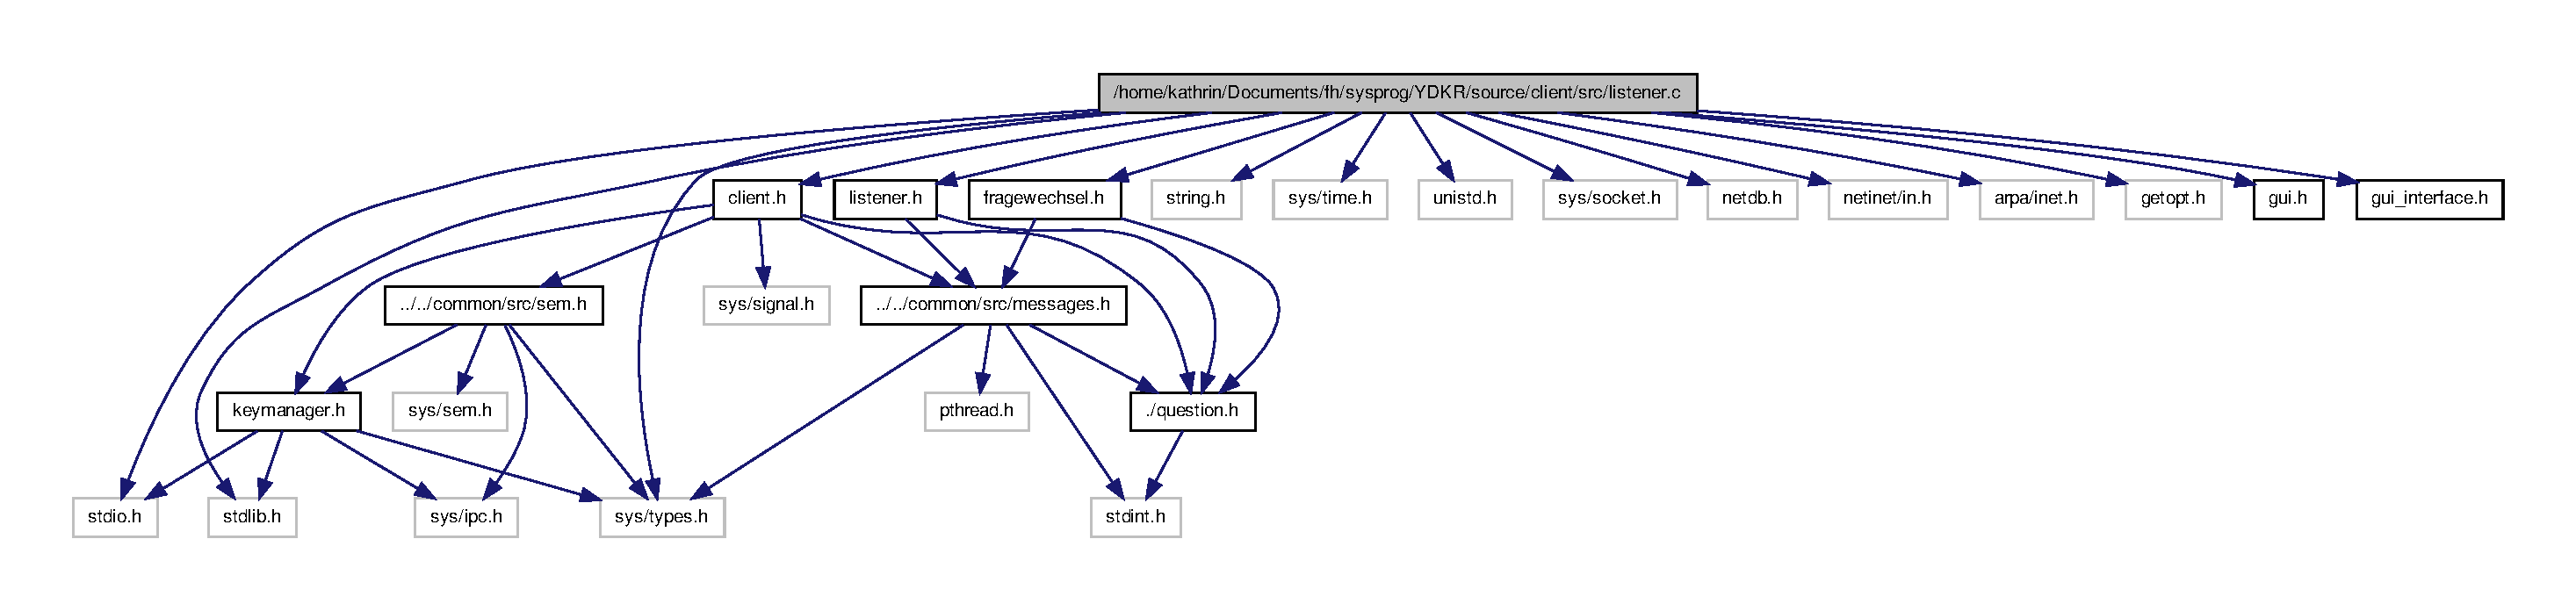
\includegraphics[width=400pt]{listener_8c__incl}
\end{center}
\end{figure}
\subsection*{Functions}
\begin{DoxyCompactItemize}
\item 
void $\ast$ \hyperlink{listener_8c_aa643c8c2955aaec54cffd88624cdf33e}{listener\_\-thread} (void $\ast$data)
\begin{DoxyCompactList}\small\item\em listener thread, gets all the packages from the server \item\end{DoxyCompactList}\item 
int \hyperlink{listener_8c_aebdd61e703b387f936a7214b62ff438f}{parse\_\-msg} (\hyperlink{structmsg__header}{t\_\-msg\_\-header} $\ast$hdr)
\begin{DoxyCompactList}\small\item\em function to parse messages from the server \item\end{DoxyCompactList}\end{DoxyCompactItemize}
\subsection*{Variables}
\begin{DoxyCompactItemize}
\item 
pthread\_\-t \hyperlink{listener_8c_ae6298cc9f112ae19ebd05c7edc7dbe8a}{question\_\-thread\_\-id}
\end{DoxyCompactItemize}


\subsection{Detailed Description}
============================================================================

\begin{DoxyAuthor}{Author}
: Kathrin Holzmann 
\end{DoxyAuthor}
\begin{DoxyDate}{Date}
: May 16, 2011 ============================================================================ 
\end{DoxyDate}


\subsection{Function Documentation}
\hypertarget{listener_8c_aa643c8c2955aaec54cffd88624cdf33e}{
\index{listener.c@{listener.c}!listener\_\-thread@{listener\_\-thread}}
\index{listener\_\-thread@{listener\_\-thread}!listener.c@{listener.c}}
\subsubsection[{listener\_\-thread}]{\setlength{\rightskip}{0pt plus 5cm}void$\ast$ listener\_\-thread (
\begin{DoxyParamCaption}
\item[{void $\ast$}]{data}
\end{DoxyParamCaption}
)}}
\label{listener_8c_aa643c8c2955aaec54cffd88624cdf33e}


listener thread, gets all the packages from the server 

=============================================================== 
\begin{DoxyParams}{Parameters}
{\em void:$\ast$data} & ============================================================== \\
\hline
\end{DoxyParams}
\hypertarget{listener_8c_aebdd61e703b387f936a7214b62ff438f}{
\index{listener.c@{listener.c}!parse\_\-msg@{parse\_\-msg}}
\index{parse\_\-msg@{parse\_\-msg}!listener.c@{listener.c}}
\subsubsection[{parse\_\-msg}]{\setlength{\rightskip}{0pt plus 5cm}int parse\_\-msg (
\begin{DoxyParamCaption}
\item[{{\bf t\_\-msg\_\-header} $\ast$}]{hdr}
\end{DoxyParamCaption}
)}}
\label{listener_8c_aebdd61e703b387f936a7214b62ff438f}


function to parse messages from the server 

================================================== 
\begin{DoxyParams}{Parameters}
{\em header:$\ast$t\_\-msg\_\-header} & ================================================= \\
\hline
\end{DoxyParams}


\subsection{Variable Documentation}
\hypertarget{listener_8c_ae6298cc9f112ae19ebd05c7edc7dbe8a}{
\index{listener.c@{listener.c}!question\_\-thread\_\-id@{question\_\-thread\_\-id}}
\index{question\_\-thread\_\-id@{question\_\-thread\_\-id}!listener.c@{listener.c}}
\subsubsection[{question\_\-thread\_\-id}]{\setlength{\rightskip}{0pt plus 5cm}pthread\_\-t {\bf question\_\-thread\_\-id}}}
\label{listener_8c_ae6298cc9f112ae19ebd05c7edc7dbe8a}

\hypertarget{listener_8h}{
\section{/home/kathrin/Documents/fh/sysprog/YDKR/source/client/src/listener.h File Reference}
\label{listener_8h}\index{/home/kathrin/Documents/fh/sysprog/YDKR/source/client/src/listener.h@{/home/kathrin/Documents/fh/sysprog/YDKR/source/client/src/listener.h}}
}
{\ttfamily \#include \char`\"{}../../common/src/messages.h\char`\"{}}\par
{\ttfamily \#include \char`\"{}../../common/src/question.h\char`\"{}}\par
Include dependency graph for listener.h:
\nopagebreak
\begin{figure}[H]
\begin{center}
\leavevmode
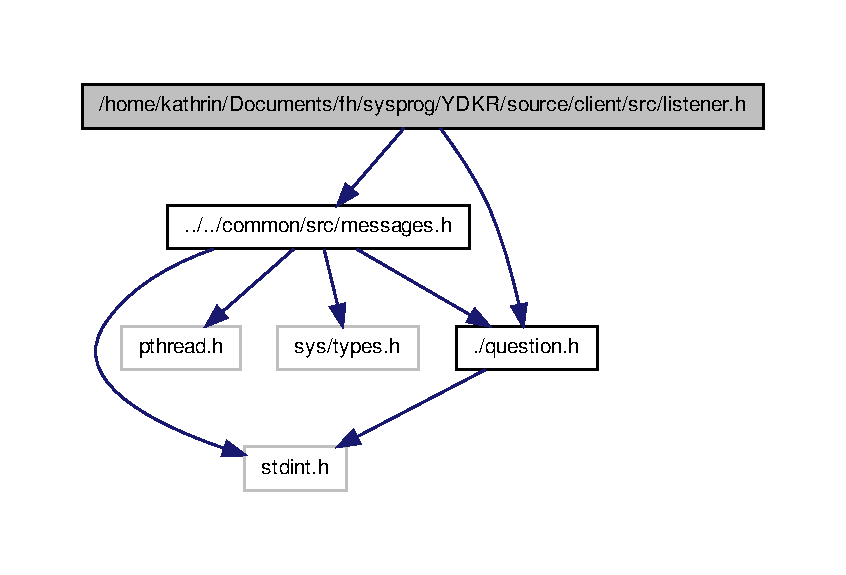
\includegraphics[width=400pt]{listener_8h__incl}
\end{center}
\end{figure}
This graph shows which files directly or indirectly include this file:
\nopagebreak
\begin{figure}[H]
\begin{center}
\leavevmode
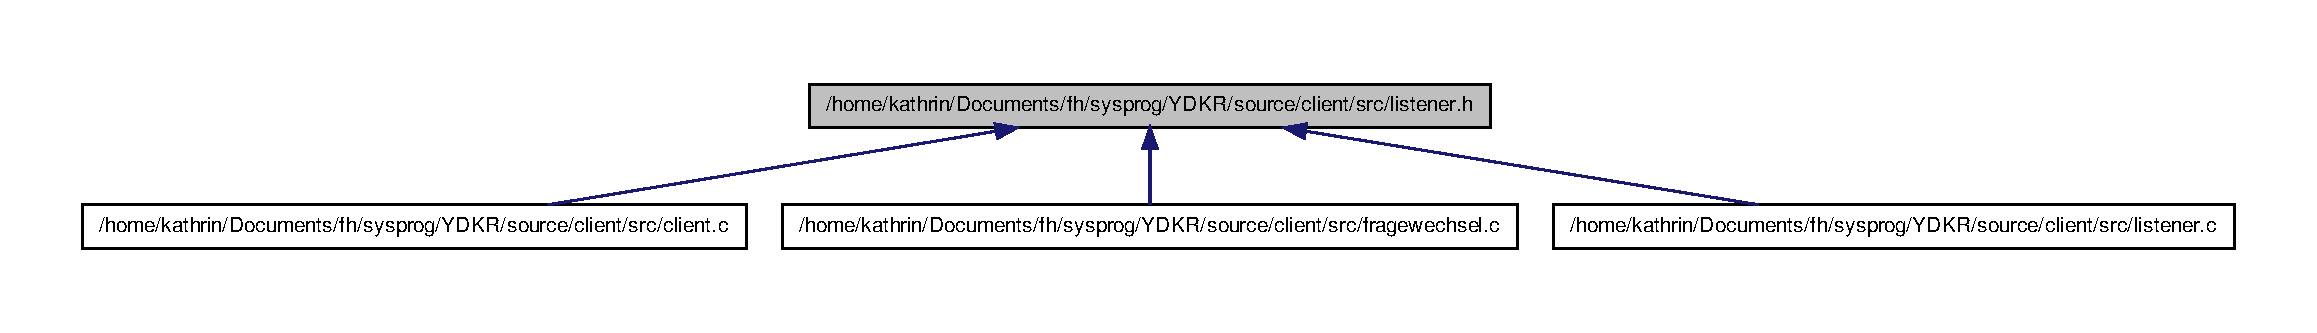
\includegraphics[width=400pt]{listener_8h__dep__incl}
\end{center}
\end{figure}
\subsection*{Data Structures}
\begin{DoxyCompactItemize}
\item 
struct \hyperlink{structquestion_result}{questionResult}
\end{DoxyCompactItemize}
\subsection*{Functions}
\begin{DoxyCompactItemize}
\item 
void $\ast$ \hyperlink{listener_8h_aa643c8c2955aaec54cffd88624cdf33e}{listener\_\-thread} (void $\ast$data)
\begin{DoxyCompactList}\small\item\em listener thread, gets all the packages from the server \item\end{DoxyCompactList}\item 
int \hyperlink{listener_8h_aebdd61e703b387f936a7214b62ff438f}{parse\_\-msg} (\hyperlink{structmsg__header}{t\_\-msg\_\-header} $\ast$hdr)
\begin{DoxyCompactList}\small\item\em function to parse messages from the server \item\end{DoxyCompactList}\item 
void \hyperlink{listener_8h_a5d90826c17597ce32adf4c0e37c98e5e}{preparation\_\-refresh\_\-playerlist} (\hyperlink{structmsg__header}{t\_\-msg\_\-header} $\ast$hdr)
\end{DoxyCompactItemize}


\subsection{Function Documentation}
\hypertarget{listener_8h_aa643c8c2955aaec54cffd88624cdf33e}{
\index{listener.h@{listener.h}!listener\_\-thread@{listener\_\-thread}}
\index{listener\_\-thread@{listener\_\-thread}!listener.h@{listener.h}}
\subsubsection[{listener\_\-thread}]{\setlength{\rightskip}{0pt plus 5cm}void$\ast$ listener\_\-thread (
\begin{DoxyParamCaption}
\item[{void $\ast$}]{data}
\end{DoxyParamCaption}
)}}
\label{listener_8h_aa643c8c2955aaec54cffd88624cdf33e}


listener thread, gets all the packages from the server 

=============================================================== 
\begin{DoxyParams}{Parameters}
{\em void:$\ast$data} & ============================================================== \\
\hline
\end{DoxyParams}
\hypertarget{listener_8h_aebdd61e703b387f936a7214b62ff438f}{
\index{listener.h@{listener.h}!parse\_\-msg@{parse\_\-msg}}
\index{parse\_\-msg@{parse\_\-msg}!listener.h@{listener.h}}
\subsubsection[{parse\_\-msg}]{\setlength{\rightskip}{0pt plus 5cm}int parse\_\-msg (
\begin{DoxyParamCaption}
\item[{{\bf t\_\-msg\_\-header} $\ast$}]{hdr}
\end{DoxyParamCaption}
)}}
\label{listener_8h_aebdd61e703b387f936a7214b62ff438f}


function to parse messages from the server 

================================================== 
\begin{DoxyParams}{Parameters}
{\em header:$\ast$t\_\-msg\_\-header} & ================================================= \\
\hline
\end{DoxyParams}
\hypertarget{listener_8h_a5d90826c17597ce32adf4c0e37c98e5e}{
\index{listener.h@{listener.h}!preparation\_\-refresh\_\-playerlist@{preparation\_\-refresh\_\-playerlist}}
\index{preparation\_\-refresh\_\-playerlist@{preparation\_\-refresh\_\-playerlist}!listener.h@{listener.h}}
\subsubsection[{preparation\_\-refresh\_\-playerlist}]{\setlength{\rightskip}{0pt plus 5cm}void preparation\_\-refresh\_\-playerlist (
\begin{DoxyParamCaption}
\item[{{\bf t\_\-msg\_\-header} $\ast$}]{hdr}
\end{DoxyParamCaption}
)}}
\label{listener_8h_a5d90826c17597ce32adf4c0e37c98e5e}

\hypertarget{keymanager_8c}{
\section{/home/kathrin/Documents/fh/sysprog/YDKR/source/common/src/keymanager.c File Reference}
\label{keymanager_8c}\index{/home/kathrin/Documents/fh/sysprog/YDKR/source/common/src/keymanager.c@{/home/kathrin/Documents/fh/sysprog/YDKR/source/common/src/keymanager.c}}
}
{\ttfamily \#include $<$unistd.h$>$}\par
{\ttfamily \#include \char`\"{}keymanager.h\char`\"{}}\par
Include dependency graph for keymanager.c:
\nopagebreak
\begin{figure}[H]
\begin{center}
\leavevmode
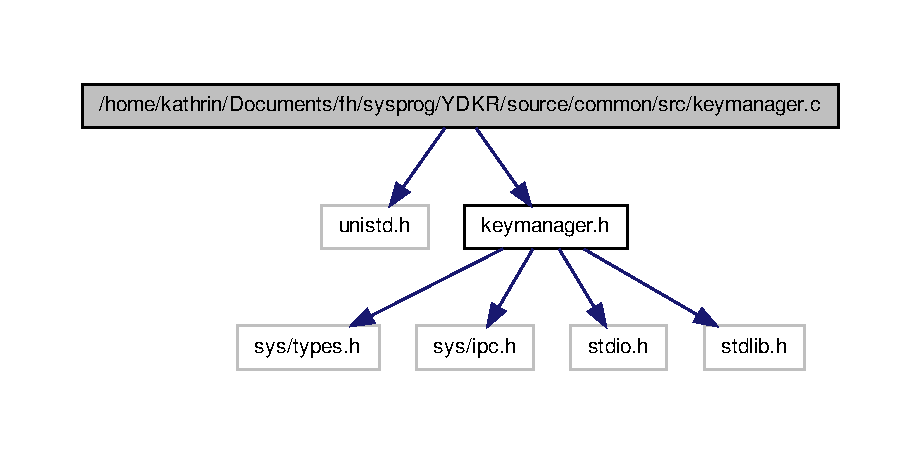
\includegraphics[width=400pt]{keymanager_8c__incl}
\end{center}
\end{figure}
\subsection*{Functions}
\begin{DoxyCompactItemize}
\item 
key\_\-t \hyperlink{keymanager_8c_a77e0ec3d1a2c477ad576e1af0b8fa19e}{keymng} (int offset)
\item 
key\_\-t \hyperlink{keymanager_8c_acd307105c0de9b745d2caf7aff6d7f45}{keymng\_\-local} (int offset)
\end{DoxyCompactItemize}


\subsection{Detailed Description}
============================================================================

\begin{DoxyAuthor}{Author}
: Kathrin Holzmann 
\end{DoxyAuthor}
\begin{DoxyDate}{Date}
: May 12, 2011 ============================================================================ 
\end{DoxyDate}


\subsection{Function Documentation}
\hypertarget{keymanager_8c_a77e0ec3d1a2c477ad576e1af0b8fa19e}{
\index{keymanager.c@{keymanager.c}!keymng@{keymng}}
\index{keymng@{keymng}!keymanager.c@{keymanager.c}}
\subsubsection[{keymng}]{\setlength{\rightskip}{0pt plus 5cm}key\_\-t keymng (
\begin{DoxyParamCaption}
\item[{int}]{offset}
\end{DoxyParamCaption}
)}}
\label{keymanager_8c_a77e0ec3d1a2c477ad576e1af0b8fa19e}
\hypertarget{keymanager_8c_acd307105c0de9b745d2caf7aff6d7f45}{
\index{keymanager.c@{keymanager.c}!keymng\_\-local@{keymng\_\-local}}
\index{keymng\_\-local@{keymng\_\-local}!keymanager.c@{keymanager.c}}
\subsubsection[{keymng\_\-local}]{\setlength{\rightskip}{0pt plus 5cm}key\_\-t keymng\_\-local (
\begin{DoxyParamCaption}
\item[{int}]{offset}
\end{DoxyParamCaption}
)}}
\label{keymanager_8c_acd307105c0de9b745d2caf7aff6d7f45}

\hypertarget{keymanager_8h}{
\section{/home/kathrin/Documents/fh/sysprog/YDKR/source/common/src/keymanager.h File Reference}
\label{keymanager_8h}\index{/home/kathrin/Documents/fh/sysprog/YDKR/source/common/src/keymanager.h@{/home/kathrin/Documents/fh/sysprog/YDKR/source/common/src/keymanager.h}}
}
{\ttfamily \#include $<$sys/types.h$>$}\par
{\ttfamily \#include $<$sys/ipc.h$>$}\par
{\ttfamily \#include $<$stdio.h$>$}\par
{\ttfamily \#include $<$stdlib.h$>$}\par
Include dependency graph for keymanager.h:
\nopagebreak
\begin{figure}[H]
\begin{center}
\leavevmode
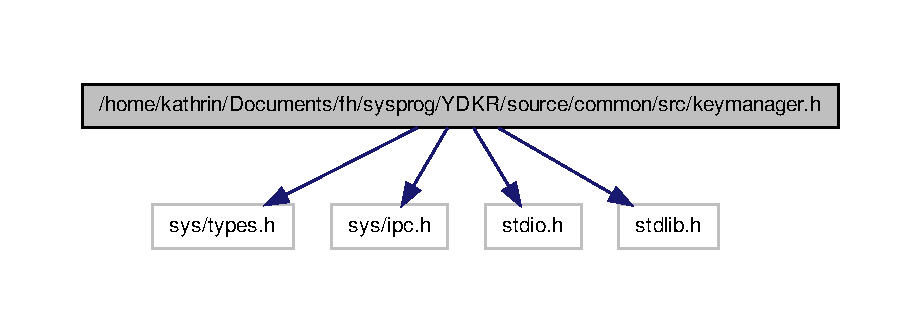
\includegraphics[width=400pt]{keymanager_8h__incl}
\end{center}
\end{figure}
This graph shows which files directly or indirectly include this file:
\nopagebreak
\begin{figure}[H]
\begin{center}
\leavevmode
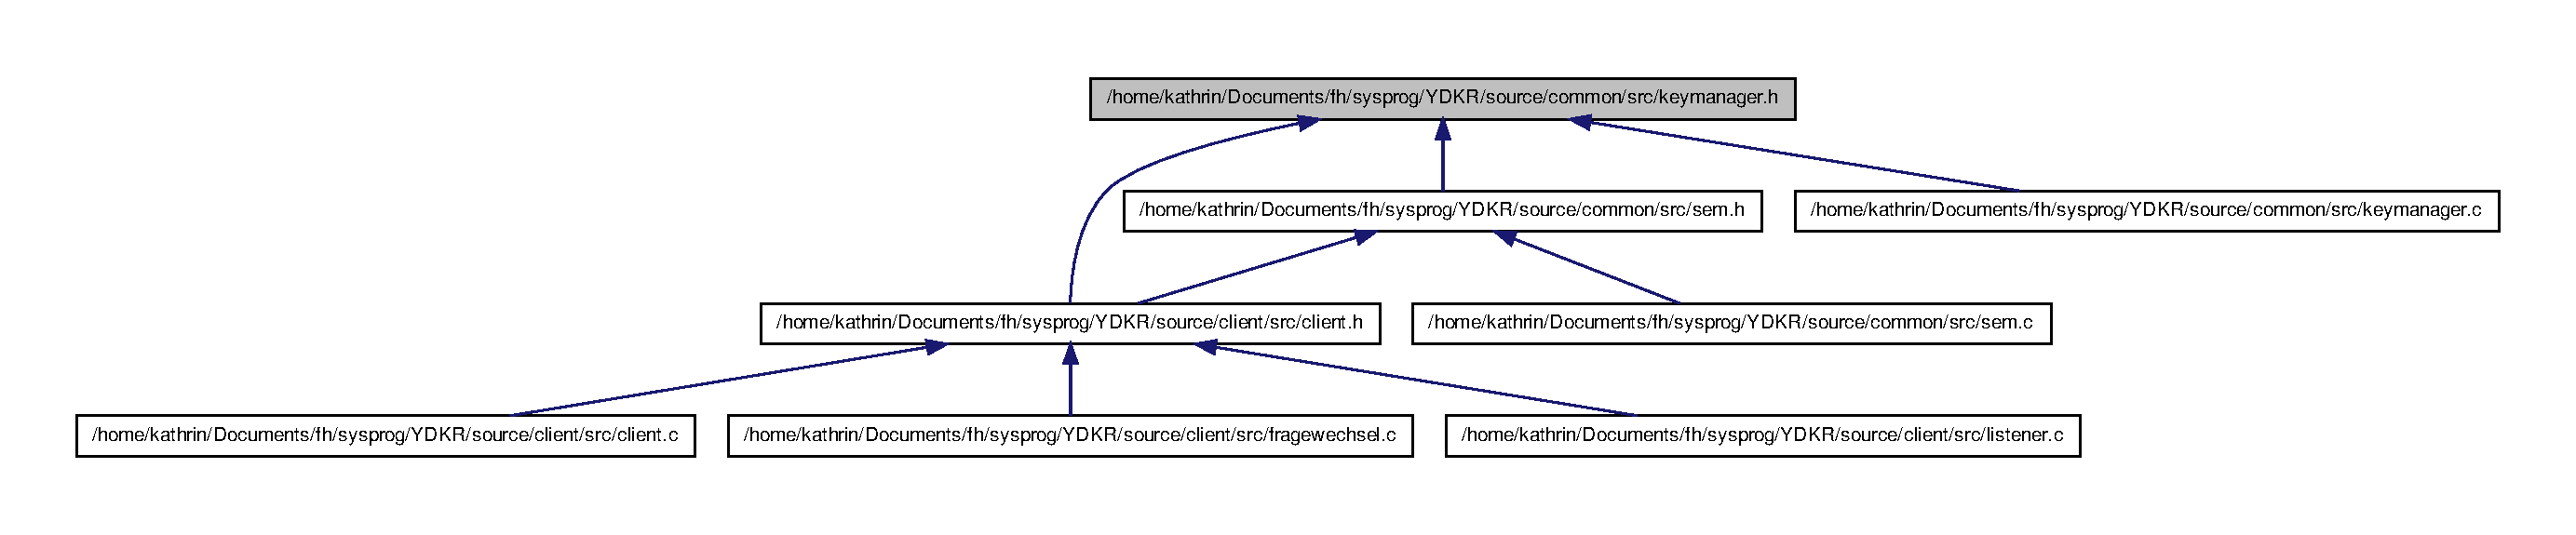
\includegraphics[width=400pt]{keymanager_8h__dep__incl}
\end{center}
\end{figure}
\subsection*{Defines}
\begin{DoxyCompactItemize}
\item 
\#define \hyperlink{keymanager_8h_ab771bcecf77941d1a588b0625fd4d1bb}{KEY\_\-GCI\_\-SEM}~0x42
\item 
\#define \hyperlink{keymanager_8h_aa9e5a514b5a73d06614bcfe54635251f}{KEY\_\-GCISOCK\_\-SEM}~0x23
\item 
\#define \hyperlink{keymanager_8h_ad4ad91532da4ae5e6efeec6b91fb7c99}{KEY\_\-COMMAND\_\-MQ}~0x41
\item 
\#define \hyperlink{keymanager_8h_a3420736b242b9ea2ad402f629fdca240}{KEY\_\-RANKING}~0x44
\item 
\#define \hyperlink{keymanager_8h_a3727ebd605eebecd9823d39a0426eef0}{KEY\_\-QUESTION}~0x43
\end{DoxyCompactItemize}
\subsection*{Functions}
\begin{DoxyCompactItemize}
\item 
key\_\-t \hyperlink{keymanager_8h_a77e0ec3d1a2c477ad576e1af0b8fa19e}{keymng} (int offset)
\item 
key\_\-t \hyperlink{keymanager_8h_acd307105c0de9b745d2caf7aff6d7f45}{keymng\_\-local} (int offset)
\end{DoxyCompactItemize}


\subsection{Define Documentation}
\hypertarget{keymanager_8h_ad4ad91532da4ae5e6efeec6b91fb7c99}{
\index{keymanager.h@{keymanager.h}!KEY\_\-COMMAND\_\-MQ@{KEY\_\-COMMAND\_\-MQ}}
\index{KEY\_\-COMMAND\_\-MQ@{KEY\_\-COMMAND\_\-MQ}!keymanager.h@{keymanager.h}}
\subsubsection[{KEY\_\-COMMAND\_\-MQ}]{\setlength{\rightskip}{0pt plus 5cm}\#define KEY\_\-COMMAND\_\-MQ~0x41}}
\label{keymanager_8h_ad4ad91532da4ae5e6efeec6b91fb7c99}
\hypertarget{keymanager_8h_ab771bcecf77941d1a588b0625fd4d1bb}{
\index{keymanager.h@{keymanager.h}!KEY\_\-GCI\_\-SEM@{KEY\_\-GCI\_\-SEM}}
\index{KEY\_\-GCI\_\-SEM@{KEY\_\-GCI\_\-SEM}!keymanager.h@{keymanager.h}}
\subsubsection[{KEY\_\-GCI\_\-SEM}]{\setlength{\rightskip}{0pt plus 5cm}\#define KEY\_\-GCI\_\-SEM~0x42}}
\label{keymanager_8h_ab771bcecf77941d1a588b0625fd4d1bb}
\hypertarget{keymanager_8h_aa9e5a514b5a73d06614bcfe54635251f}{
\index{keymanager.h@{keymanager.h}!KEY\_\-GCISOCK\_\-SEM@{KEY\_\-GCISOCK\_\-SEM}}
\index{KEY\_\-GCISOCK\_\-SEM@{KEY\_\-GCISOCK\_\-SEM}!keymanager.h@{keymanager.h}}
\subsubsection[{KEY\_\-GCISOCK\_\-SEM}]{\setlength{\rightskip}{0pt plus 5cm}\#define KEY\_\-GCISOCK\_\-SEM~0x23}}
\label{keymanager_8h_aa9e5a514b5a73d06614bcfe54635251f}
\hypertarget{keymanager_8h_a3727ebd605eebecd9823d39a0426eef0}{
\index{keymanager.h@{keymanager.h}!KEY\_\-QUESTION@{KEY\_\-QUESTION}}
\index{KEY\_\-QUESTION@{KEY\_\-QUESTION}!keymanager.h@{keymanager.h}}
\subsubsection[{KEY\_\-QUESTION}]{\setlength{\rightskip}{0pt plus 5cm}\#define KEY\_\-QUESTION~0x43}}
\label{keymanager_8h_a3727ebd605eebecd9823d39a0426eef0}
\hypertarget{keymanager_8h_a3420736b242b9ea2ad402f629fdca240}{
\index{keymanager.h@{keymanager.h}!KEY\_\-RANKING@{KEY\_\-RANKING}}
\index{KEY\_\-RANKING@{KEY\_\-RANKING}!keymanager.h@{keymanager.h}}
\subsubsection[{KEY\_\-RANKING}]{\setlength{\rightskip}{0pt plus 5cm}\#define KEY\_\-RANKING~0x44}}
\label{keymanager_8h_a3420736b242b9ea2ad402f629fdca240}


\subsection{Function Documentation}
\hypertarget{keymanager_8h_a77e0ec3d1a2c477ad576e1af0b8fa19e}{
\index{keymanager.h@{keymanager.h}!keymng@{keymng}}
\index{keymng@{keymng}!keymanager.h@{keymanager.h}}
\subsubsection[{keymng}]{\setlength{\rightskip}{0pt plus 5cm}key\_\-t keymng (
\begin{DoxyParamCaption}
\item[{int}]{offset}
\end{DoxyParamCaption}
)}}
\label{keymanager_8h_a77e0ec3d1a2c477ad576e1af0b8fa19e}
\hypertarget{keymanager_8h_acd307105c0de9b745d2caf7aff6d7f45}{
\index{keymanager.h@{keymanager.h}!keymng\_\-local@{keymng\_\-local}}
\index{keymng\_\-local@{keymng\_\-local}!keymanager.h@{keymanager.h}}
\subsubsection[{keymng\_\-local}]{\setlength{\rightskip}{0pt plus 5cm}key\_\-t keymng\_\-local (
\begin{DoxyParamCaption}
\item[{int}]{offset}
\end{DoxyParamCaption}
)}}
\label{keymanager_8h_acd307105c0de9b745d2caf7aff6d7f45}

\hypertarget{messages_8h}{
\section{/home/kathrin/Documents/fh/sysprog/YDKR/source/common/src/messages.h File Reference}
\label{messages_8h}\index{/home/kathrin/Documents/fh/sysprog/YDKR/source/common/src/messages.h@{/home/kathrin/Documents/fh/sysprog/YDKR/source/common/src/messages.h}}
}
{\ttfamily \#include $<$stdint.h$>$}\par
{\ttfamily \#include $<$pthread.h$>$}\par
{\ttfamily \#include $<$sys/types.h$>$}\par
{\ttfamily \#include \char`\"{}./question.h\char`\"{}}\par
Include dependency graph for messages.h:
\nopagebreak
\begin{figure}[H]
\begin{center}
\leavevmode
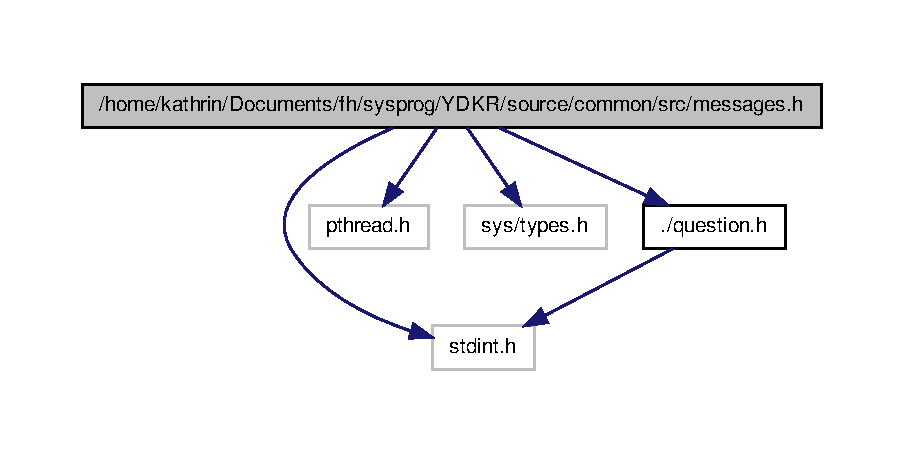
\includegraphics[width=400pt]{messages_8h__incl}
\end{center}
\end{figure}
This graph shows which files directly or indirectly include this file:
\nopagebreak
\begin{figure}[H]
\begin{center}
\leavevmode
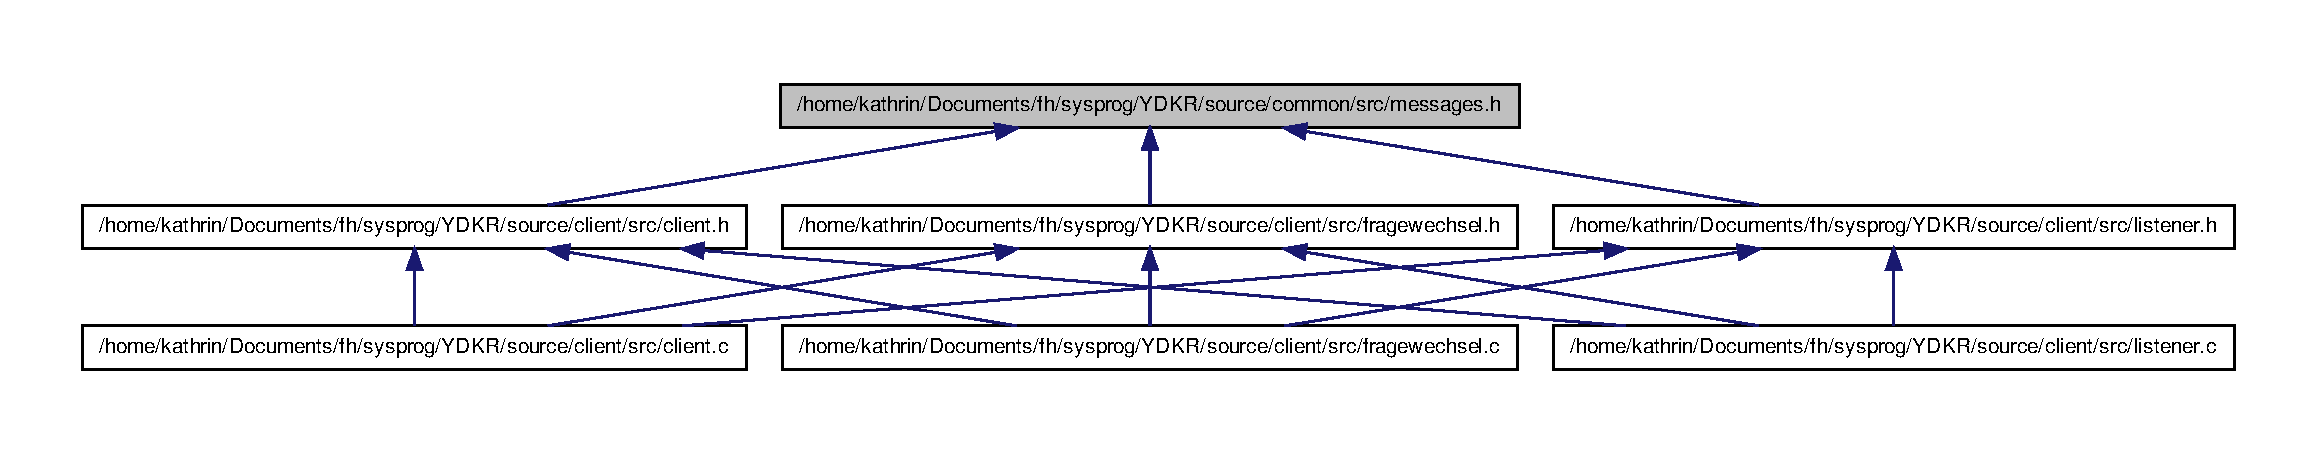
\includegraphics[width=400pt]{messages_8h__dep__incl}
\end{center}
\end{figure}
\subsection*{Data Structures}
\begin{DoxyCompactItemize}
\item 
struct \hyperlink{structmsg__header}{msg\_\-header}
\item 
struct \hyperlink{structlogin__request}{login\_\-request}
\item 
struct \hyperlink{structlogin__response___o_k}{login\_\-response\_\-OK}
\item 
struct \hyperlink{structplayer__list}{player\_\-list}
\item 
struct \hyperlink{structcatalog__request}{catalog\_\-request}
\item 
struct \hyperlink{structcatalog__response}{catalog\_\-response}
\item 
struct \hyperlink{structcatalog__change}{catalog\_\-change}
\item 
struct \hyperlink{structstart__game}{start\_\-game}
\item 
struct \hyperlink{structquestion__request}{question\_\-request}
\item 
struct \hyperlink{structquestion}{question}
\item 
struct \hyperlink{structquestion__answered}{question\_\-answered}
\item 
struct \hyperlink{structquestion__result}{question\_\-result}
\item 
struct \hyperlink{structgame__over}{game\_\-over}
\item 
struct \hyperlink{structerror__warning}{error\_\-warning}
\end{DoxyCompactItemize}
\subsection*{Defines}
\begin{DoxyCompactItemize}
\item 
\#define \hyperlink{messages_8h_a1dce0e03c9ad36ace3b6192e1f69c4b2}{RFC\_\-LOGINREQUEST}~1
\item 
\#define \hyperlink{messages_8h_a45b9b014ea9cc4ef53c723f68e005155}{RFC\_\-LOGINRESPONSEOK}~2
\item 
\#define \hyperlink{messages_8h_a86bdfb4ab44ef7e31369b4f2e63fd804}{RFC\_\-PLAYERLIST}~3
\item 
\#define \hyperlink{messages_8h_a78ec98552d512af077794e628d26bbff}{RFC\_\-CATALOGREQUEST}~4
\item 
\#define \hyperlink{messages_8h_a226bfe026ade1e70c3b4f1eca76618b8}{RFC\_\-CATALOGRESPONSE}~5
\item 
\#define \hyperlink{messages_8h_a6225ab7262f316cf4ae061bbf42fae67}{RFC\_\-CATALOGCHANGE}~6
\item 
\#define \hyperlink{messages_8h_adaa36364e6b312fc72bd6f004d78e44a}{RFC\_\-STARTGAME}~7
\item 
\#define \hyperlink{messages_8h_a7d74d25e41201fdf9b4b9685a5532b6c}{RFC\_\-QUESTIONREQUEST}~8
\item 
\#define \hyperlink{messages_8h_a79910d3b948a09c05033c15e6988db1d}{RFC\_\-QUESTION}~9
\item 
\#define \hyperlink{messages_8h_ac16eb304e7b4fcff8869e554ebedbe48}{RFC\_\-QUESTIONANSWERED}~10
\item 
\#define \hyperlink{messages_8h_adef6e89b5167278719247404b62fc4a4}{RFC\_\-QUESTIONRESULT}~11
\item 
\#define \hyperlink{messages_8h_afd976df8169e258638dee8ccf57cabcb}{RFC\_\-GAMEOVER}~12
\item 
\#define \hyperlink{messages_8h_af8bd9e4dd08de7f461fa72b44d487d4a}{RFC\_\-ERRORWARNING}~255
\item 
\#define \hyperlink{messages_8h_a0e61edf18ebeac89626cb0baaaf18365}{RFC\_\-ROLE\_\-DONTCARE}~0
\item 
\#define \hyperlink{messages_8h_afd1dc013168eaca5364d87988e1746df}{RFC\_\-ROLE\_\-SLAVE}~1
\item 
\#define \hyperlink{messages_8h_abf9400f93d4872de85ad9b2aca7e4376}{RFC\_\-ROLE\_\-MASTER}~2
\item 
\#define \hyperlink{messages_8h_acd89697454b504d241e47086e959196a}{RFC\_\-ERROR\_\-WARN}~0
\item 
\#define \hyperlink{messages_8h_ac59ceeedd4d699fe4f5d5d66f563e725}{RFC\_\-ERROR\_\-FATAL}~1
\item 
\#define \hyperlink{messages_8h_ae523111e3b55fe5c0022c35a979b3a02}{RFC\_\-ERROR\_\-LOGIN\_\-FAIL}~10
\end{DoxyCompactItemize}
\subsection*{Typedefs}
\begin{DoxyCompactItemize}
\item 
typedef struct \hyperlink{structmsg__header}{msg\_\-header} \hyperlink{messages_8h_a2a441fa9aad06caf96bf752aa747b454}{t\_\-msg\_\-header}
\item 
typedef struct \hyperlink{structlogin__request}{login\_\-request} \hyperlink{messages_8h_aac05ebc44380cbae5856e58ba5522a6b}{LOGINREQUEST}
\item 
typedef struct \hyperlink{structlogin__response___o_k}{login\_\-response\_\-OK} \hyperlink{messages_8h_adac20f2e95f9c8429fa76ad73f0419f1}{LOGINRESPONSEOK}
\item 
typedef struct \hyperlink{structplayer__list}{player\_\-list} \hyperlink{messages_8h_a101b2c6e8fbcc6b4ed575ad1cc62cada}{PLAYERLIST}
\item 
typedef struct \hyperlink{structplayer__list}{player\_\-list} \hyperlink{messages_8h_a0e23d35bd42753b72472b8abf0ca7a4c}{playerls}
\item 
typedef struct \hyperlink{structcatalog__request}{catalog\_\-request} \hyperlink{messages_8h_ac459784b82e78c11fec927c2e43e5811}{CATALOGREQUEST}
\item 
typedef struct \hyperlink{structcatalog__request}{catalog\_\-request} \hyperlink{messages_8h_a8b9a864b59bdf979c8fea4dd168c8d0b}{catareq}
\item 
typedef struct \hyperlink{structcatalog__response}{catalog\_\-response} \hyperlink{messages_8h_ad7bf6bbd12b4949d92231a71bdb31821}{CATALOGRESPONSE}
\item 
typedef struct \hyperlink{structcatalog__response}{catalog\_\-response} \hyperlink{messages_8h_a2a5dd0eb5fa32b1d467928ae2bb9c54b}{catares}
\item 
typedef struct \hyperlink{structcatalog__change}{catalog\_\-change} \hyperlink{messages_8h_af9d5f8f515366cca46765027b901fcde}{CATALOGCHANGE}
\item 
typedef struct \hyperlink{structcatalog__change}{catalog\_\-change} \hyperlink{messages_8h_aad134b225615d6c89d9a3669f05c61ca}{catach}
\item 
typedef struct \hyperlink{structstart__game}{start\_\-game} \hyperlink{messages_8h_ac9b0984540d87d2a7042613a1dd55c71}{STARTGAME}
\item 
typedef struct \hyperlink{structstart__game}{start\_\-game} \hyperlink{messages_8h_a8eb2f7d1015f2a5493f63b916ce09a15}{startgm}
\item 
typedef struct \hyperlink{structquestion__request}{question\_\-request} \hyperlink{messages_8h_ab12610bbbb5fb4ed4d10125caae29520}{QUESTIONREQUEST}
\item 
typedef struct \hyperlink{structquestion__request}{question\_\-request} \hyperlink{messages_8h_a4a336b540e903a537da72d9db8311e9a}{questionreq}
\item 
typedef struct \hyperlink{structquestion}{question} \hyperlink{messages_8h_abb8fbc5152b7015dcec9e67091e5e846}{QUESTION}
\item 
typedef struct \hyperlink{structquestion__answered}{question\_\-answered} \hyperlink{messages_8h_a71d62bd0a2427c2e39390a6b8811b448}{QUESTIONANSWERED}
\item 
typedef struct \hyperlink{structquestion__result}{question\_\-result} \hyperlink{messages_8h_a009828b79dccfea860e8f5e367e459dd}{QUESTIONRESULT}
\item 
typedef struct \hyperlink{structgame__over}{game\_\-over} \hyperlink{messages_8h_ad98ecd36579207a26dfcccd96a207368}{GAMEOVER}
\item 
typedef struct \hyperlink{structerror__warning}{error\_\-warning} \hyperlink{messages_8h_ae7da5395e49e5c1f5e229d73e5d22e70}{ERRORWARNING}
\end{DoxyCompactItemize}
\subsection*{Functions}
\begin{DoxyCompactItemize}
\item 
struct \hyperlink{structmsg__header}{msg\_\-header} \hyperlink{messages_8h_aefe298f440566dcc65ae47c848d82514}{\_\-\_\-attribute\_\-\_\-} ((\_\-\_\-packed\_\-\_\-))
\end{DoxyCompactItemize}
\subsection*{Variables}
\begin{DoxyCompactItemize}
\item 
uint8\_\-t \hyperlink{messages_8h_a1d127017fb298b889f4ba24752d08b8e}{type}
\item 
uint16\_\-t \hyperlink{messages_8h_a1892eba2086d12ac2b09005aeb09ea3b}{length}
\end{DoxyCompactItemize}


\subsection{Detailed Description}
============================================================================

\begin{DoxyAuthor}{Author}
: Kathrin Holzmann 
\end{DoxyAuthor}
\begin{DoxyDate}{Date}
: May 12, 2011 ============================================================================ 
\end{DoxyDate}


\subsection{Define Documentation}
\hypertarget{messages_8h_a6225ab7262f316cf4ae061bbf42fae67}{
\index{messages.h@{messages.h}!RFC\_\-CATALOGCHANGE@{RFC\_\-CATALOGCHANGE}}
\index{RFC\_\-CATALOGCHANGE@{RFC\_\-CATALOGCHANGE}!messages.h@{messages.h}}
\subsubsection[{RFC\_\-CATALOGCHANGE}]{\setlength{\rightskip}{0pt plus 5cm}\#define RFC\_\-CATALOGCHANGE~6}}
\label{messages_8h_a6225ab7262f316cf4ae061bbf42fae67}
\hypertarget{messages_8h_a78ec98552d512af077794e628d26bbff}{
\index{messages.h@{messages.h}!RFC\_\-CATALOGREQUEST@{RFC\_\-CATALOGREQUEST}}
\index{RFC\_\-CATALOGREQUEST@{RFC\_\-CATALOGREQUEST}!messages.h@{messages.h}}
\subsubsection[{RFC\_\-CATALOGREQUEST}]{\setlength{\rightskip}{0pt plus 5cm}\#define RFC\_\-CATALOGREQUEST~4}}
\label{messages_8h_a78ec98552d512af077794e628d26bbff}
\hypertarget{messages_8h_a226bfe026ade1e70c3b4f1eca76618b8}{
\index{messages.h@{messages.h}!RFC\_\-CATALOGRESPONSE@{RFC\_\-CATALOGRESPONSE}}
\index{RFC\_\-CATALOGRESPONSE@{RFC\_\-CATALOGRESPONSE}!messages.h@{messages.h}}
\subsubsection[{RFC\_\-CATALOGRESPONSE}]{\setlength{\rightskip}{0pt plus 5cm}\#define RFC\_\-CATALOGRESPONSE~5}}
\label{messages_8h_a226bfe026ade1e70c3b4f1eca76618b8}
\hypertarget{messages_8h_ac59ceeedd4d699fe4f5d5d66f563e725}{
\index{messages.h@{messages.h}!RFC\_\-ERROR\_\-FATAL@{RFC\_\-ERROR\_\-FATAL}}
\index{RFC\_\-ERROR\_\-FATAL@{RFC\_\-ERROR\_\-FATAL}!messages.h@{messages.h}}
\subsubsection[{RFC\_\-ERROR\_\-FATAL}]{\setlength{\rightskip}{0pt plus 5cm}\#define RFC\_\-ERROR\_\-FATAL~1}}
\label{messages_8h_ac59ceeedd4d699fe4f5d5d66f563e725}
\hypertarget{messages_8h_ae523111e3b55fe5c0022c35a979b3a02}{
\index{messages.h@{messages.h}!RFC\_\-ERROR\_\-LOGIN\_\-FAIL@{RFC\_\-ERROR\_\-LOGIN\_\-FAIL}}
\index{RFC\_\-ERROR\_\-LOGIN\_\-FAIL@{RFC\_\-ERROR\_\-LOGIN\_\-FAIL}!messages.h@{messages.h}}
\subsubsection[{RFC\_\-ERROR\_\-LOGIN\_\-FAIL}]{\setlength{\rightskip}{0pt plus 5cm}\#define RFC\_\-ERROR\_\-LOGIN\_\-FAIL~10}}
\label{messages_8h_ae523111e3b55fe5c0022c35a979b3a02}
\hypertarget{messages_8h_acd89697454b504d241e47086e959196a}{
\index{messages.h@{messages.h}!RFC\_\-ERROR\_\-WARN@{RFC\_\-ERROR\_\-WARN}}
\index{RFC\_\-ERROR\_\-WARN@{RFC\_\-ERROR\_\-WARN}!messages.h@{messages.h}}
\subsubsection[{RFC\_\-ERROR\_\-WARN}]{\setlength{\rightskip}{0pt plus 5cm}\#define RFC\_\-ERROR\_\-WARN~0}}
\label{messages_8h_acd89697454b504d241e47086e959196a}
\hypertarget{messages_8h_af8bd9e4dd08de7f461fa72b44d487d4a}{
\index{messages.h@{messages.h}!RFC\_\-ERRORWARNING@{RFC\_\-ERRORWARNING}}
\index{RFC\_\-ERRORWARNING@{RFC\_\-ERRORWARNING}!messages.h@{messages.h}}
\subsubsection[{RFC\_\-ERRORWARNING}]{\setlength{\rightskip}{0pt plus 5cm}\#define RFC\_\-ERRORWARNING~255}}
\label{messages_8h_af8bd9e4dd08de7f461fa72b44d487d4a}
\hypertarget{messages_8h_afd976df8169e258638dee8ccf57cabcb}{
\index{messages.h@{messages.h}!RFC\_\-GAMEOVER@{RFC\_\-GAMEOVER}}
\index{RFC\_\-GAMEOVER@{RFC\_\-GAMEOVER}!messages.h@{messages.h}}
\subsubsection[{RFC\_\-GAMEOVER}]{\setlength{\rightskip}{0pt plus 5cm}\#define RFC\_\-GAMEOVER~12}}
\label{messages_8h_afd976df8169e258638dee8ccf57cabcb}
\hypertarget{messages_8h_a1dce0e03c9ad36ace3b6192e1f69c4b2}{
\index{messages.h@{messages.h}!RFC\_\-LOGINREQUEST@{RFC\_\-LOGINREQUEST}}
\index{RFC\_\-LOGINREQUEST@{RFC\_\-LOGINREQUEST}!messages.h@{messages.h}}
\subsubsection[{RFC\_\-LOGINREQUEST}]{\setlength{\rightskip}{0pt plus 5cm}\#define RFC\_\-LOGINREQUEST~1}}
\label{messages_8h_a1dce0e03c9ad36ace3b6192e1f69c4b2}
\hypertarget{messages_8h_a45b9b014ea9cc4ef53c723f68e005155}{
\index{messages.h@{messages.h}!RFC\_\-LOGINRESPONSEOK@{RFC\_\-LOGINRESPONSEOK}}
\index{RFC\_\-LOGINRESPONSEOK@{RFC\_\-LOGINRESPONSEOK}!messages.h@{messages.h}}
\subsubsection[{RFC\_\-LOGINRESPONSEOK}]{\setlength{\rightskip}{0pt plus 5cm}\#define RFC\_\-LOGINRESPONSEOK~2}}
\label{messages_8h_a45b9b014ea9cc4ef53c723f68e005155}
\hypertarget{messages_8h_a86bdfb4ab44ef7e31369b4f2e63fd804}{
\index{messages.h@{messages.h}!RFC\_\-PLAYERLIST@{RFC\_\-PLAYERLIST}}
\index{RFC\_\-PLAYERLIST@{RFC\_\-PLAYERLIST}!messages.h@{messages.h}}
\subsubsection[{RFC\_\-PLAYERLIST}]{\setlength{\rightskip}{0pt plus 5cm}\#define RFC\_\-PLAYERLIST~3}}
\label{messages_8h_a86bdfb4ab44ef7e31369b4f2e63fd804}
\hypertarget{messages_8h_a79910d3b948a09c05033c15e6988db1d}{
\index{messages.h@{messages.h}!RFC\_\-QUESTION@{RFC\_\-QUESTION}}
\index{RFC\_\-QUESTION@{RFC\_\-QUESTION}!messages.h@{messages.h}}
\subsubsection[{RFC\_\-QUESTION}]{\setlength{\rightskip}{0pt plus 5cm}\#define RFC\_\-QUESTION~9}}
\label{messages_8h_a79910d3b948a09c05033c15e6988db1d}
\hypertarget{messages_8h_ac16eb304e7b4fcff8869e554ebedbe48}{
\index{messages.h@{messages.h}!RFC\_\-QUESTIONANSWERED@{RFC\_\-QUESTIONANSWERED}}
\index{RFC\_\-QUESTIONANSWERED@{RFC\_\-QUESTIONANSWERED}!messages.h@{messages.h}}
\subsubsection[{RFC\_\-QUESTIONANSWERED}]{\setlength{\rightskip}{0pt plus 5cm}\#define RFC\_\-QUESTIONANSWERED~10}}
\label{messages_8h_ac16eb304e7b4fcff8869e554ebedbe48}
\hypertarget{messages_8h_a7d74d25e41201fdf9b4b9685a5532b6c}{
\index{messages.h@{messages.h}!RFC\_\-QUESTIONREQUEST@{RFC\_\-QUESTIONREQUEST}}
\index{RFC\_\-QUESTIONREQUEST@{RFC\_\-QUESTIONREQUEST}!messages.h@{messages.h}}
\subsubsection[{RFC\_\-QUESTIONREQUEST}]{\setlength{\rightskip}{0pt plus 5cm}\#define RFC\_\-QUESTIONREQUEST~8}}
\label{messages_8h_a7d74d25e41201fdf9b4b9685a5532b6c}
\hypertarget{messages_8h_adef6e89b5167278719247404b62fc4a4}{
\index{messages.h@{messages.h}!RFC\_\-QUESTIONRESULT@{RFC\_\-QUESTIONRESULT}}
\index{RFC\_\-QUESTIONRESULT@{RFC\_\-QUESTIONRESULT}!messages.h@{messages.h}}
\subsubsection[{RFC\_\-QUESTIONRESULT}]{\setlength{\rightskip}{0pt plus 5cm}\#define RFC\_\-QUESTIONRESULT~11}}
\label{messages_8h_adef6e89b5167278719247404b62fc4a4}
\hypertarget{messages_8h_a0e61edf18ebeac89626cb0baaaf18365}{
\index{messages.h@{messages.h}!RFC\_\-ROLE\_\-DONTCARE@{RFC\_\-ROLE\_\-DONTCARE}}
\index{RFC\_\-ROLE\_\-DONTCARE@{RFC\_\-ROLE\_\-DONTCARE}!messages.h@{messages.h}}
\subsubsection[{RFC\_\-ROLE\_\-DONTCARE}]{\setlength{\rightskip}{0pt plus 5cm}\#define RFC\_\-ROLE\_\-DONTCARE~0}}
\label{messages_8h_a0e61edf18ebeac89626cb0baaaf18365}
\hypertarget{messages_8h_abf9400f93d4872de85ad9b2aca7e4376}{
\index{messages.h@{messages.h}!RFC\_\-ROLE\_\-MASTER@{RFC\_\-ROLE\_\-MASTER}}
\index{RFC\_\-ROLE\_\-MASTER@{RFC\_\-ROLE\_\-MASTER}!messages.h@{messages.h}}
\subsubsection[{RFC\_\-ROLE\_\-MASTER}]{\setlength{\rightskip}{0pt plus 5cm}\#define RFC\_\-ROLE\_\-MASTER~2}}
\label{messages_8h_abf9400f93d4872de85ad9b2aca7e4376}
\hypertarget{messages_8h_afd1dc013168eaca5364d87988e1746df}{
\index{messages.h@{messages.h}!RFC\_\-ROLE\_\-SLAVE@{RFC\_\-ROLE\_\-SLAVE}}
\index{RFC\_\-ROLE\_\-SLAVE@{RFC\_\-ROLE\_\-SLAVE}!messages.h@{messages.h}}
\subsubsection[{RFC\_\-ROLE\_\-SLAVE}]{\setlength{\rightskip}{0pt plus 5cm}\#define RFC\_\-ROLE\_\-SLAVE~1}}
\label{messages_8h_afd1dc013168eaca5364d87988e1746df}
\hypertarget{messages_8h_adaa36364e6b312fc72bd6f004d78e44a}{
\index{messages.h@{messages.h}!RFC\_\-STARTGAME@{RFC\_\-STARTGAME}}
\index{RFC\_\-STARTGAME@{RFC\_\-STARTGAME}!messages.h@{messages.h}}
\subsubsection[{RFC\_\-STARTGAME}]{\setlength{\rightskip}{0pt plus 5cm}\#define RFC\_\-STARTGAME~7}}
\label{messages_8h_adaa36364e6b312fc72bd6f004d78e44a}


\subsection{Typedef Documentation}
\hypertarget{messages_8h_aad134b225615d6c89d9a3669f05c61ca}{
\index{messages.h@{messages.h}!catach@{catach}}
\index{catach@{catach}!messages.h@{messages.h}}
\subsubsection[{catach}]{\setlength{\rightskip}{0pt plus 5cm}typedef struct {\bf catalog\_\-change} {\bf catach}}}
\label{messages_8h_aad134b225615d6c89d9a3669f05c61ca}
\hypertarget{messages_8h_af9d5f8f515366cca46765027b901fcde}{
\index{messages.h@{messages.h}!CATALOGCHANGE@{CATALOGCHANGE}}
\index{CATALOGCHANGE@{CATALOGCHANGE}!messages.h@{messages.h}}
\subsubsection[{CATALOGCHANGE}]{\setlength{\rightskip}{0pt plus 5cm}typedef struct {\bf catalog\_\-change} {\bf CATALOGCHANGE}}}
\label{messages_8h_af9d5f8f515366cca46765027b901fcde}
\hypertarget{messages_8h_ac459784b82e78c11fec927c2e43e5811}{
\index{messages.h@{messages.h}!CATALOGREQUEST@{CATALOGREQUEST}}
\index{CATALOGREQUEST@{CATALOGREQUEST}!messages.h@{messages.h}}
\subsubsection[{CATALOGREQUEST}]{\setlength{\rightskip}{0pt plus 5cm}typedef struct {\bf catalog\_\-request} {\bf CATALOGREQUEST}}}
\label{messages_8h_ac459784b82e78c11fec927c2e43e5811}
\hypertarget{messages_8h_ad7bf6bbd12b4949d92231a71bdb31821}{
\index{messages.h@{messages.h}!CATALOGRESPONSE@{CATALOGRESPONSE}}
\index{CATALOGRESPONSE@{CATALOGRESPONSE}!messages.h@{messages.h}}
\subsubsection[{CATALOGRESPONSE}]{\setlength{\rightskip}{0pt plus 5cm}typedef struct {\bf catalog\_\-response} {\bf CATALOGRESPONSE}}}
\label{messages_8h_ad7bf6bbd12b4949d92231a71bdb31821}
\hypertarget{messages_8h_a8b9a864b59bdf979c8fea4dd168c8d0b}{
\index{messages.h@{messages.h}!catareq@{catareq}}
\index{catareq@{catareq}!messages.h@{messages.h}}
\subsubsection[{catareq}]{\setlength{\rightskip}{0pt plus 5cm}typedef struct {\bf catalog\_\-request} {\bf catareq}}}
\label{messages_8h_a8b9a864b59bdf979c8fea4dd168c8d0b}
\hypertarget{messages_8h_a2a5dd0eb5fa32b1d467928ae2bb9c54b}{
\index{messages.h@{messages.h}!catares@{catares}}
\index{catares@{catares}!messages.h@{messages.h}}
\subsubsection[{catares}]{\setlength{\rightskip}{0pt plus 5cm}typedef struct {\bf catalog\_\-response} {\bf catares}}}
\label{messages_8h_a2a5dd0eb5fa32b1d467928ae2bb9c54b}
\hypertarget{messages_8h_ae7da5395e49e5c1f5e229d73e5d22e70}{
\index{messages.h@{messages.h}!ERRORWARNING@{ERRORWARNING}}
\index{ERRORWARNING@{ERRORWARNING}!messages.h@{messages.h}}
\subsubsection[{ERRORWARNING}]{\setlength{\rightskip}{0pt plus 5cm}typedef struct {\bf error\_\-warning} {\bf ERRORWARNING}}}
\label{messages_8h_ae7da5395e49e5c1f5e229d73e5d22e70}
\hypertarget{messages_8h_ad98ecd36579207a26dfcccd96a207368}{
\index{messages.h@{messages.h}!GAMEOVER@{GAMEOVER}}
\index{GAMEOVER@{GAMEOVER}!messages.h@{messages.h}}
\subsubsection[{GAMEOVER}]{\setlength{\rightskip}{0pt plus 5cm}typedef struct {\bf game\_\-over} {\bf GAMEOVER}}}
\label{messages_8h_ad98ecd36579207a26dfcccd96a207368}
\hypertarget{messages_8h_aac05ebc44380cbae5856e58ba5522a6b}{
\index{messages.h@{messages.h}!LOGINREQUEST@{LOGINREQUEST}}
\index{LOGINREQUEST@{LOGINREQUEST}!messages.h@{messages.h}}
\subsubsection[{LOGINREQUEST}]{\setlength{\rightskip}{0pt plus 5cm}typedef struct {\bf login\_\-request} {\bf LOGINREQUEST}}}
\label{messages_8h_aac05ebc44380cbae5856e58ba5522a6b}
\hypertarget{messages_8h_adac20f2e95f9c8429fa76ad73f0419f1}{
\index{messages.h@{messages.h}!LOGINRESPONSEOK@{LOGINRESPONSEOK}}
\index{LOGINRESPONSEOK@{LOGINRESPONSEOK}!messages.h@{messages.h}}
\subsubsection[{LOGINRESPONSEOK}]{\setlength{\rightskip}{0pt plus 5cm}typedef struct {\bf login\_\-response\_\-OK} {\bf LOGINRESPONSEOK}}}
\label{messages_8h_adac20f2e95f9c8429fa76ad73f0419f1}
\hypertarget{messages_8h_a101b2c6e8fbcc6b4ed575ad1cc62cada}{
\index{messages.h@{messages.h}!PLAYERLIST@{PLAYERLIST}}
\index{PLAYERLIST@{PLAYERLIST}!messages.h@{messages.h}}
\subsubsection[{PLAYERLIST}]{\setlength{\rightskip}{0pt plus 5cm}typedef struct {\bf player\_\-list} {\bf PLAYERLIST}}}
\label{messages_8h_a101b2c6e8fbcc6b4ed575ad1cc62cada}
\hypertarget{messages_8h_a0e23d35bd42753b72472b8abf0ca7a4c}{
\index{messages.h@{messages.h}!playerls@{playerls}}
\index{playerls@{playerls}!messages.h@{messages.h}}
\subsubsection[{playerls}]{\setlength{\rightskip}{0pt plus 5cm}typedef struct {\bf player\_\-list} {\bf playerls}}}
\label{messages_8h_a0e23d35bd42753b72472b8abf0ca7a4c}
\hypertarget{messages_8h_abb8fbc5152b7015dcec9e67091e5e846}{
\index{messages.h@{messages.h}!QUESTION@{QUESTION}}
\index{QUESTION@{QUESTION}!messages.h@{messages.h}}
\subsubsection[{QUESTION}]{\setlength{\rightskip}{0pt plus 5cm}typedef struct {\bf question} {\bf QUESTION}}}
\label{messages_8h_abb8fbc5152b7015dcec9e67091e5e846}
\hypertarget{messages_8h_a71d62bd0a2427c2e39390a6b8811b448}{
\index{messages.h@{messages.h}!QUESTIONANSWERED@{QUESTIONANSWERED}}
\index{QUESTIONANSWERED@{QUESTIONANSWERED}!messages.h@{messages.h}}
\subsubsection[{QUESTIONANSWERED}]{\setlength{\rightskip}{0pt plus 5cm}typedef struct {\bf question\_\-answered} {\bf QUESTIONANSWERED}}}
\label{messages_8h_a71d62bd0a2427c2e39390a6b8811b448}
\hypertarget{messages_8h_a4a336b540e903a537da72d9db8311e9a}{
\index{messages.h@{messages.h}!questionreq@{questionreq}}
\index{questionreq@{questionreq}!messages.h@{messages.h}}
\subsubsection[{questionreq}]{\setlength{\rightskip}{0pt plus 5cm}typedef struct {\bf question\_\-request} {\bf questionreq}}}
\label{messages_8h_a4a336b540e903a537da72d9db8311e9a}
\hypertarget{messages_8h_ab12610bbbb5fb4ed4d10125caae29520}{
\index{messages.h@{messages.h}!QUESTIONREQUEST@{QUESTIONREQUEST}}
\index{QUESTIONREQUEST@{QUESTIONREQUEST}!messages.h@{messages.h}}
\subsubsection[{QUESTIONREQUEST}]{\setlength{\rightskip}{0pt plus 5cm}typedef struct {\bf question\_\-request} {\bf QUESTIONREQUEST}}}
\label{messages_8h_ab12610bbbb5fb4ed4d10125caae29520}
\hypertarget{messages_8h_a009828b79dccfea860e8f5e367e459dd}{
\index{messages.h@{messages.h}!QUESTIONRESULT@{QUESTIONRESULT}}
\index{QUESTIONRESULT@{QUESTIONRESULT}!messages.h@{messages.h}}
\subsubsection[{QUESTIONRESULT}]{\setlength{\rightskip}{0pt plus 5cm}typedef struct {\bf question\_\-result} {\bf QUESTIONRESULT}}}
\label{messages_8h_a009828b79dccfea860e8f5e367e459dd}
\hypertarget{messages_8h_ac9b0984540d87d2a7042613a1dd55c71}{
\index{messages.h@{messages.h}!STARTGAME@{STARTGAME}}
\index{STARTGAME@{STARTGAME}!messages.h@{messages.h}}
\subsubsection[{STARTGAME}]{\setlength{\rightskip}{0pt plus 5cm}typedef struct {\bf start\_\-game} {\bf STARTGAME}}}
\label{messages_8h_ac9b0984540d87d2a7042613a1dd55c71}
\hypertarget{messages_8h_a8eb2f7d1015f2a5493f63b916ce09a15}{
\index{messages.h@{messages.h}!startgm@{startgm}}
\index{startgm@{startgm}!messages.h@{messages.h}}
\subsubsection[{startgm}]{\setlength{\rightskip}{0pt plus 5cm}typedef struct {\bf start\_\-game} {\bf startgm}}}
\label{messages_8h_a8eb2f7d1015f2a5493f63b916ce09a15}
\hypertarget{messages_8h_a2a441fa9aad06caf96bf752aa747b454}{
\index{messages.h@{messages.h}!t\_\-msg\_\-header@{t\_\-msg\_\-header}}
\index{t\_\-msg\_\-header@{t\_\-msg\_\-header}!messages.h@{messages.h}}
\subsubsection[{t\_\-msg\_\-header}]{\setlength{\rightskip}{0pt plus 5cm}typedef struct {\bf msg\_\-header} {\bf t\_\-msg\_\-header}}}
\label{messages_8h_a2a441fa9aad06caf96bf752aa747b454}


\subsection{Function Documentation}
\hypertarget{messages_8h_aefe298f440566dcc65ae47c848d82514}{
\index{messages.h@{messages.h}!\_\-\_\-attribute\_\-\_\-@{\_\-\_\-attribute\_\-\_\-}}
\index{\_\-\_\-attribute\_\-\_\-@{\_\-\_\-attribute\_\-\_\-}!messages.h@{messages.h}}
\subsubsection[{\_\-\_\-attribute\_\-\_\-}]{\setlength{\rightskip}{0pt plus 5cm}struct {\bf msg\_\-header} \_\-\_\-attribute\_\-\_\- (
\begin{DoxyParamCaption}
\item[{(\_\-\_\-packed\_\-\_\-)}]{}
\end{DoxyParamCaption}
)}}
\label{messages_8h_aefe298f440566dcc65ae47c848d82514}


\subsection{Variable Documentation}
\hypertarget{messages_8h_a1892eba2086d12ac2b09005aeb09ea3b}{
\index{messages.h@{messages.h}!length@{length}}
\index{length@{length}!messages.h@{messages.h}}
\subsubsection[{length}]{\setlength{\rightskip}{0pt plus 5cm}uint16\_\-t {\bf length}}}
\label{messages_8h_a1892eba2086d12ac2b09005aeb09ea3b}
\hypertarget{messages_8h_a1d127017fb298b889f4ba24752d08b8e}{
\index{messages.h@{messages.h}!type@{type}}
\index{type@{type}!messages.h@{messages.h}}
\subsubsection[{type}]{\setlength{\rightskip}{0pt plus 5cm}uint8\_\-t {\bf type}}}
\label{messages_8h_a1d127017fb298b889f4ba24752d08b8e}

\hypertarget{question_8h}{
\section{/home/kathrin/Documents/fh/sysprog/YDKR/source/common/src/question.h File Reference}
\label{question_8h}\index{/home/kathrin/Documents/fh/sysprog/YDKR/source/common/src/question.h@{/home/kathrin/Documents/fh/sysprog/YDKR/source/common/src/question.h}}
}
{\ttfamily \#include $<$stdint.h$>$}\par
Include dependency graph for question.h:
\nopagebreak
\begin{figure}[H]
\begin{center}
\leavevmode
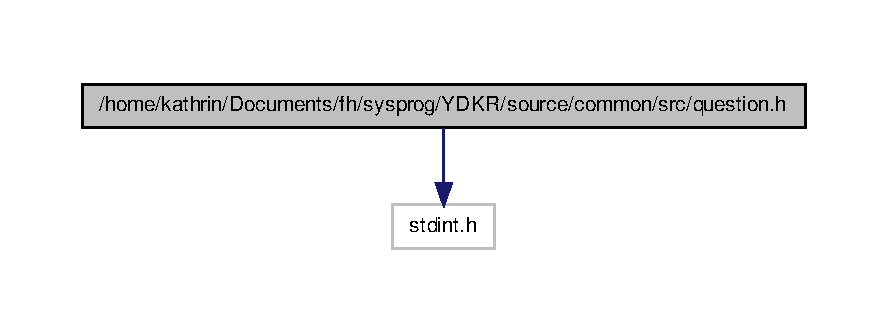
\includegraphics[width=400pt]{question_8h__incl}
\end{center}
\end{figure}
This graph shows which files directly or indirectly include this file:
\nopagebreak
\begin{figure}[H]
\begin{center}
\leavevmode
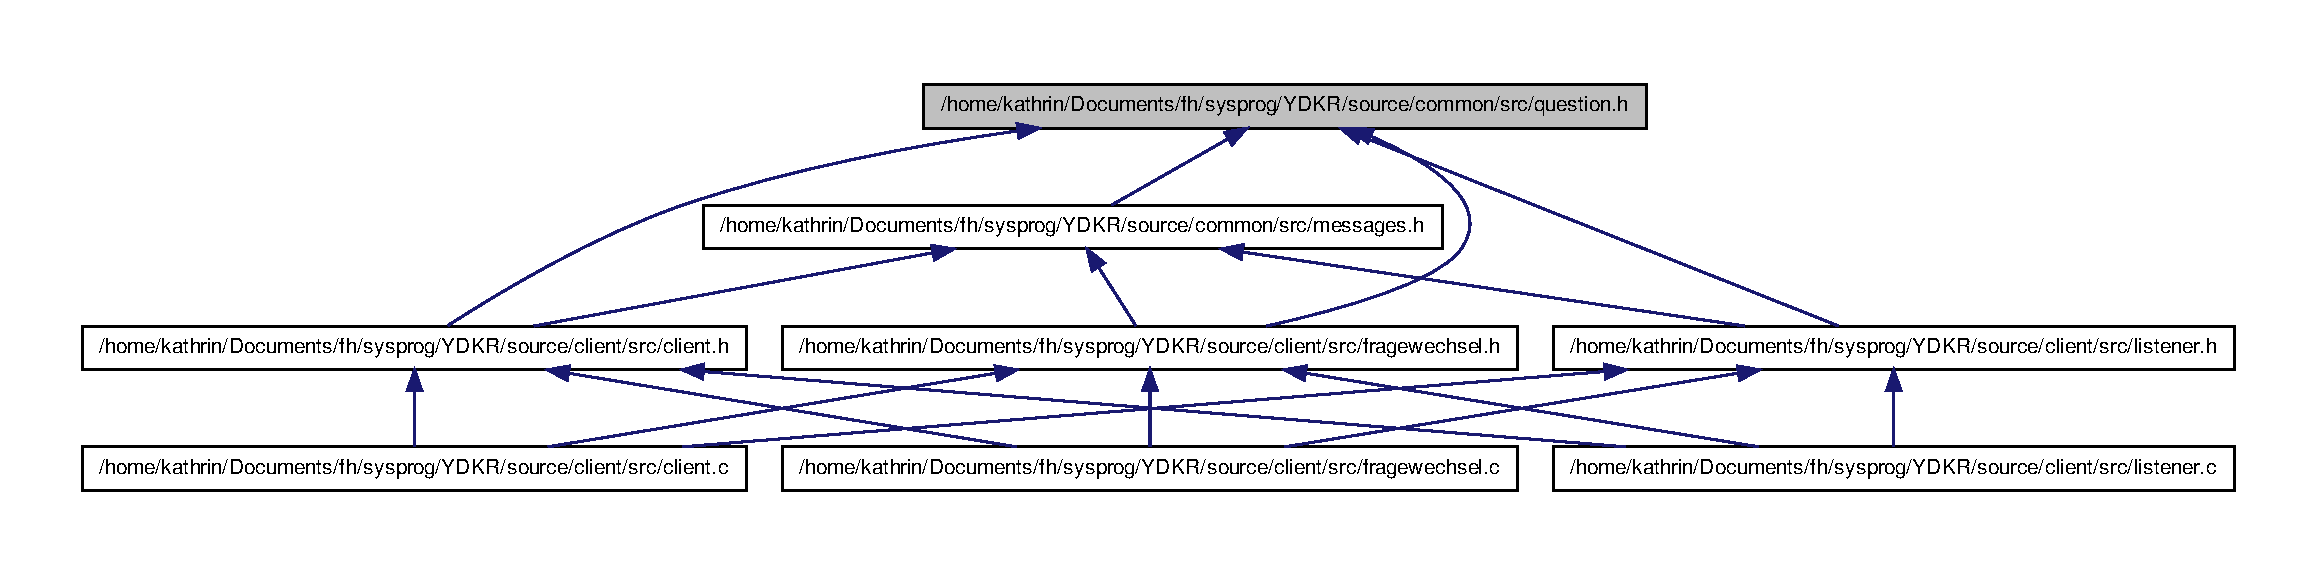
\includegraphics[width=400pt]{question_8h__dep__incl}
\end{center}
\end{figure}
\subsection*{Data Structures}
\begin{DoxyCompactItemize}
\item 
struct \hyperlink{struct_question}{Question}
\begin{DoxyCompactList}\small\item\em Interne Darstellung einer Frage. \item\end{DoxyCompactList}\item 
struct \hyperlink{struct_question_message}{QuestionMessage}
\begin{DoxyCompactList}\small\item\em Darstellung einer Frage während des Transports zum Client. \item\end{DoxyCompactList}\end{DoxyCompactItemize}
\subsection*{Enumerations}
\begin{DoxyCompactItemize}
\item 
enum \{ \hyperlink{question_8h_adf764cbdea00d65edcd07bb9953ad2b7ab7db6358972e1ff1cf5c9931ef45c547}{QUESTION\_\-SIZE} =  256, 
\hyperlink{question_8h_adf764cbdea00d65edcd07bb9953ad2b7ab318124c8ebc814e1a5337a9e18f2681}{ANSWER\_\-SIZE} =  128, 
\hyperlink{question_8h_adf764cbdea00d65edcd07bb9953ad2b7a37e5e1ac1cb8d085e53c84e8ed6514e9}{NUM\_\-ANSWERS} =  4
 \}
\end{DoxyCompactItemize}


\subsection{Enumeration Type Documentation}
\hypertarget{question_8h_adf764cbdea00d65edcd07bb9953ad2b7}{
\subsubsection[{"@1}]{\setlength{\rightskip}{0pt plus 5cm}anonymous enum}}
\label{question_8h_adf764cbdea00d65edcd07bb9953ad2b7}
\begin{Desc}
\item[Enumerator: ]\par
\begin{description}
\index{QUESTION\_\-SIZE@{QUESTION\_\-SIZE}!question.h@{question.h}}\index{question.h@{question.h}!QUESTION\_\-SIZE@{QUESTION\_\-SIZE}}\item[{\em 
\hypertarget{question_8h_adf764cbdea00d65edcd07bb9953ad2b7ab7db6358972e1ff1cf5c9931ef45c547}{
QUESTION\_\-SIZE}
\label{question_8h_adf764cbdea00d65edcd07bb9953ad2b7ab7db6358972e1ff1cf5c9931ef45c547}
}]Maximale Länge einer Frage (in Bytes) \index{ANSWER\_\-SIZE@{ANSWER\_\-SIZE}!question.h@{question.h}}\index{question.h@{question.h}!ANSWER\_\-SIZE@{ANSWER\_\-SIZE}}\item[{\em 
\hypertarget{question_8h_adf764cbdea00d65edcd07bb9953ad2b7ab318124c8ebc814e1a5337a9e18f2681}{
ANSWER\_\-SIZE}
\label{question_8h_adf764cbdea00d65edcd07bb9953ad2b7ab318124c8ebc814e1a5337a9e18f2681}
}]Maximale Länge einer Antwort (in Bytes) \index{NUM\_\-ANSWERS@{NUM\_\-ANSWERS}!question.h@{question.h}}\index{question.h@{question.h}!NUM\_\-ANSWERS@{NUM\_\-ANSWERS}}\item[{\em 
\hypertarget{question_8h_adf764cbdea00d65edcd07bb9953ad2b7a37e5e1ac1cb8d085e53c84e8ed6514e9}{
NUM\_\-ANSWERS}
\label{question_8h_adf764cbdea00d65edcd07bb9953ad2b7a37e5e1ac1cb8d085e53c84e8ed6514e9}
}]Anzahl der Antworten pro Frage \end{description}
\end{Desc}


\hypertarget{sem_8c}{
\section{/home/kathrin/Documents/fh/sysprog/YDKR/source/common/src/sem.c File Reference}
\label{sem_8c}\index{/home/kathrin/Documents/fh/sysprog/YDKR/source/common/src/sem.c@{/home/kathrin/Documents/fh/sysprog/YDKR/source/common/src/sem.c}}
}
{\ttfamily \#include $<$stdio.h$>$}\par
{\ttfamily \#include $<$signal.h$>$}\par
{\ttfamily \#include \char`\"{}sem.h\char`\"{}}\par
Include dependency graph for sem.c:
\nopagebreak
\begin{figure}[H]
\begin{center}
\leavevmode
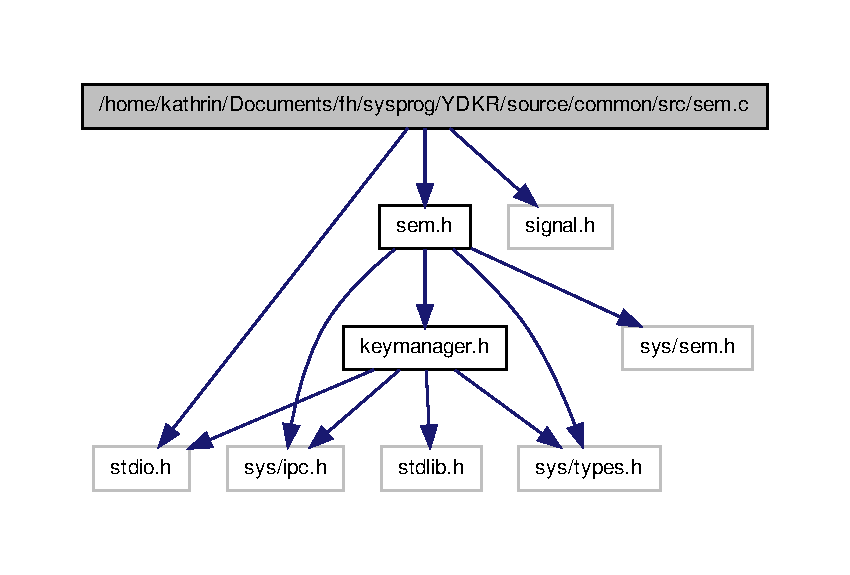
\includegraphics[width=400pt]{sem_8c__incl}
\end{center}
\end{figure}
\subsection*{Functions}
\begin{DoxyCompactItemize}
\item 
int \hyperlink{sem_8c_af5f03e4951768e97ea24e093179302ed}{sem\_\-open} (key\_\-t key)
\item 
int \hyperlink{sem_8c_a4e1dace5e69fb4881d6152ade20315ef}{sem\_\-remove} (key\_\-t key)
\item 
int \hyperlink{sem_8c_a3ef41c1f6b4d5ec30b7fccf625e565f8}{sem\_\-V} (key\_\-t key)
\item 
int \hyperlink{sem_8c_a54ab9482f44aaa75ffd80f32f8c8c75e}{sem\_\-P} (key\_\-t key)
\end{DoxyCompactItemize}


\subsection{Detailed Description}
============================================================================

\begin{DoxyAuthor}{Author}
: Kathrin Holzmann 
\end{DoxyAuthor}
\begin{DoxyDate}{Date}
: June 02, 2011 ============================================================================ 
\end{DoxyDate}


\subsection{Function Documentation}
\hypertarget{sem_8c_af5f03e4951768e97ea24e093179302ed}{
\index{sem.c@{sem.c}!sem\_\-open@{sem\_\-open}}
\index{sem\_\-open@{sem\_\-open}!sem.c@{sem.c}}
\subsubsection[{sem\_\-open}]{\setlength{\rightskip}{0pt plus 5cm}int sem\_\-open (
\begin{DoxyParamCaption}
\item[{key\_\-t}]{key}
\end{DoxyParamCaption}
)}}
\label{sem_8c_af5f03e4951768e97ea24e093179302ed}
\hypertarget{sem_8c_a54ab9482f44aaa75ffd80f32f8c8c75e}{
\index{sem.c@{sem.c}!sem\_\-P@{sem\_\-P}}
\index{sem\_\-P@{sem\_\-P}!sem.c@{sem.c}}
\subsubsection[{sem\_\-P}]{\setlength{\rightskip}{0pt plus 5cm}int sem\_\-P (
\begin{DoxyParamCaption}
\item[{key\_\-t}]{key}
\end{DoxyParamCaption}
)}}
\label{sem_8c_a54ab9482f44aaa75ffd80f32f8c8c75e}
\hypertarget{sem_8c_a4e1dace5e69fb4881d6152ade20315ef}{
\index{sem.c@{sem.c}!sem\_\-remove@{sem\_\-remove}}
\index{sem\_\-remove@{sem\_\-remove}!sem.c@{sem.c}}
\subsubsection[{sem\_\-remove}]{\setlength{\rightskip}{0pt plus 5cm}int sem\_\-remove (
\begin{DoxyParamCaption}
\item[{key\_\-t}]{key}
\end{DoxyParamCaption}
)}}
\label{sem_8c_a4e1dace5e69fb4881d6152ade20315ef}
\hypertarget{sem_8c_a3ef41c1f6b4d5ec30b7fccf625e565f8}{
\index{sem.c@{sem.c}!sem\_\-V@{sem\_\-V}}
\index{sem\_\-V@{sem\_\-V}!sem.c@{sem.c}}
\subsubsection[{sem\_\-V}]{\setlength{\rightskip}{0pt plus 5cm}int sem\_\-V (
\begin{DoxyParamCaption}
\item[{key\_\-t}]{key}
\end{DoxyParamCaption}
)}}
\label{sem_8c_a3ef41c1f6b4d5ec30b7fccf625e565f8}

\hypertarget{sem_8h}{
\section{/home/kathrin/Documents/fh/sysprog/YDKR/source/common/src/sem.h File Reference}
\label{sem_8h}\index{/home/kathrin/Documents/fh/sysprog/YDKR/source/common/src/sem.h@{/home/kathrin/Documents/fh/sysprog/YDKR/source/common/src/sem.h}}
}
{\ttfamily \#include $<$sys/sem.h$>$}\par
{\ttfamily \#include $<$sys/types.h$>$}\par
{\ttfamily \#include $<$sys/ipc.h$>$}\par
{\ttfamily \#include \char`\"{}keymanager.h\char`\"{}}\par
Include dependency graph for sem.h:
\nopagebreak
\begin{figure}[H]
\begin{center}
\leavevmode
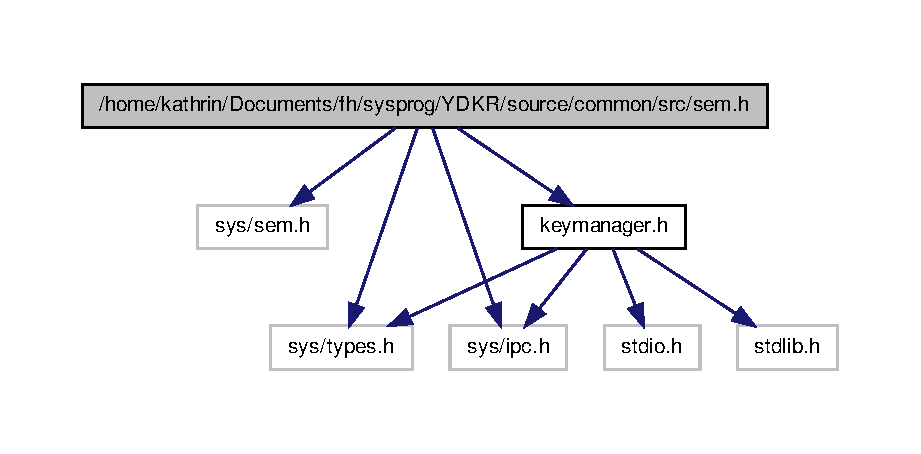
\includegraphics[width=400pt]{sem_8h__incl}
\end{center}
\end{figure}
This graph shows which files directly or indirectly include this file:
\nopagebreak
\begin{figure}[H]
\begin{center}
\leavevmode
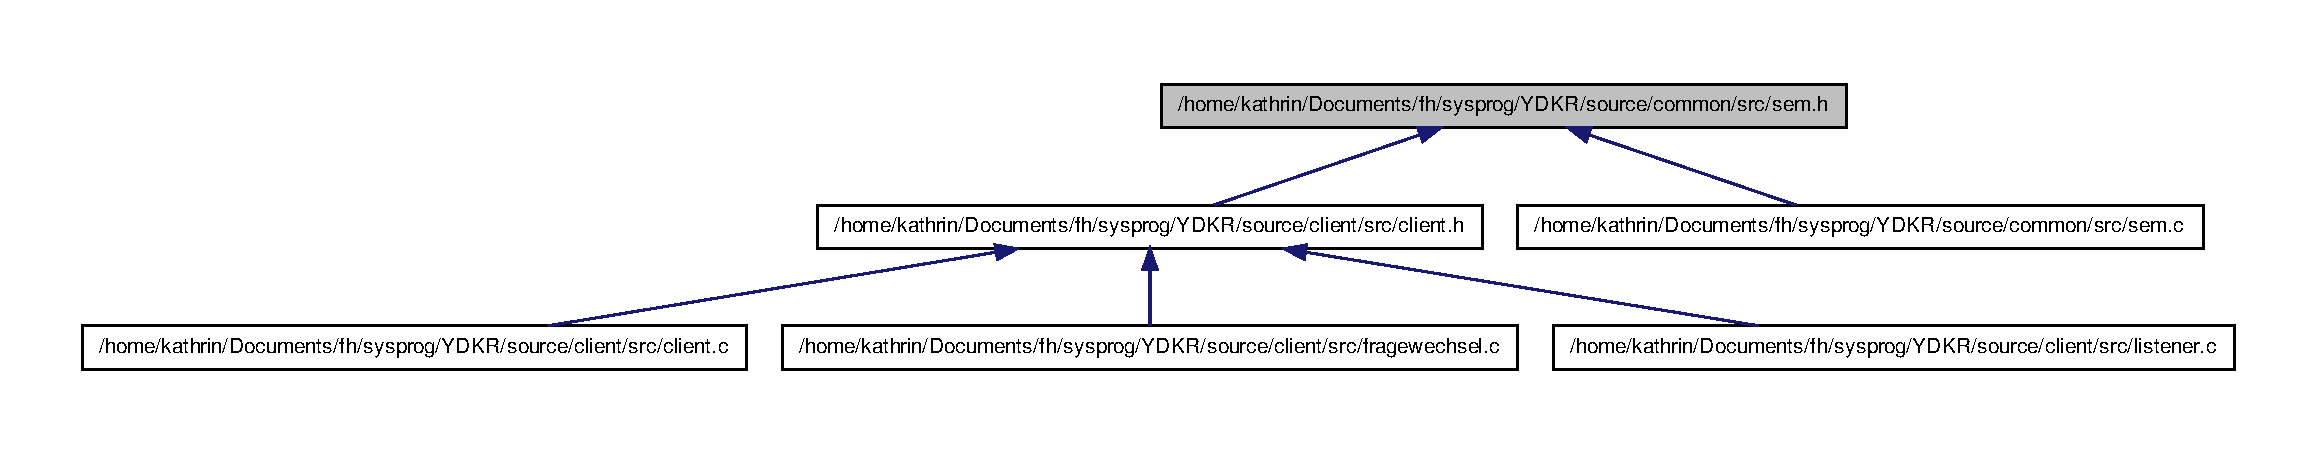
\includegraphics[width=400pt]{sem_8h__dep__incl}
\end{center}
\end{figure}
\subsection*{Functions}
\begin{DoxyCompactItemize}
\item 
int \hyperlink{sem_8h_af5f03e4951768e97ea24e093179302ed}{sem\_\-open} (key\_\-t key)
\item 
int \hyperlink{sem_8h_a4e1dace5e69fb4881d6152ade20315ef}{sem\_\-remove} (key\_\-t key)
\item 
int \hyperlink{sem_8h_a3ef41c1f6b4d5ec30b7fccf625e565f8}{sem\_\-V} (key\_\-t key)
\item 
int \hyperlink{sem_8h_a54ab9482f44aaa75ffd80f32f8c8c75e}{sem\_\-P} (key\_\-t key)
\end{DoxyCompactItemize}


\subsection{Detailed Description}
============================================================================

\begin{DoxyAuthor}{Author}
: Kathrin Holzmann 
\end{DoxyAuthor}
\begin{DoxyDate}{Date}
: June 02, 2011 ============================================================================ 
\end{DoxyDate}


\subsection{Function Documentation}
\hypertarget{sem_8h_af5f03e4951768e97ea24e093179302ed}{
\index{sem.h@{sem.h}!sem\_\-open@{sem\_\-open}}
\index{sem\_\-open@{sem\_\-open}!sem.h@{sem.h}}
\subsubsection[{sem\_\-open}]{\setlength{\rightskip}{0pt plus 5cm}int sem\_\-open (
\begin{DoxyParamCaption}
\item[{key\_\-t}]{key}
\end{DoxyParamCaption}
)}}
\label{sem_8h_af5f03e4951768e97ea24e093179302ed}
\hypertarget{sem_8h_a54ab9482f44aaa75ffd80f32f8c8c75e}{
\index{sem.h@{sem.h}!sem\_\-P@{sem\_\-P}}
\index{sem\_\-P@{sem\_\-P}!sem.h@{sem.h}}
\subsubsection[{sem\_\-P}]{\setlength{\rightskip}{0pt plus 5cm}int sem\_\-P (
\begin{DoxyParamCaption}
\item[{key\_\-t}]{key}
\end{DoxyParamCaption}
)}}
\label{sem_8h_a54ab9482f44aaa75ffd80f32f8c8c75e}
\hypertarget{sem_8h_a4e1dace5e69fb4881d6152ade20315ef}{
\index{sem.h@{sem.h}!sem\_\-remove@{sem\_\-remove}}
\index{sem\_\-remove@{sem\_\-remove}!sem.h@{sem.h}}
\subsubsection[{sem\_\-remove}]{\setlength{\rightskip}{0pt plus 5cm}int sem\_\-remove (
\begin{DoxyParamCaption}
\item[{key\_\-t}]{key}
\end{DoxyParamCaption}
)}}
\label{sem_8h_a4e1dace5e69fb4881d6152ade20315ef}
\hypertarget{sem_8h_a3ef41c1f6b4d5ec30b7fccf625e565f8}{
\index{sem.h@{sem.h}!sem\_\-V@{sem\_\-V}}
\index{sem\_\-V@{sem\_\-V}!sem.h@{sem.h}}
\subsubsection[{sem\_\-V}]{\setlength{\rightskip}{0pt plus 5cm}int sem\_\-V (
\begin{DoxyParamCaption}
\item[{key\_\-t}]{key}
\end{DoxyParamCaption}
)}}
\label{sem_8h_a3ef41c1f6b4d5ec30b7fccf625e565f8}

\printindex
\end{document}
